\documentclass[10pt]{article}
%\usepackage{url}
%\usepackage{algorithmic}
\usepackage[margin=1in]{geometry}
\usepackage{datetime}
\usepackage[margin=2em, font=footnotesize]{caption}
\usepackage{graphicx}
\usepackage{mathpazo} % use palatino
\usepackage[scaled]{helvet} % helvetica
\usepackage{microtype}
\usepackage{amsmath}
\usepackage{subfigure}
\usepackage{listings}
\usepackage{wrapfig}
\usepackage{ amssymb }
% Letterspacing macros
\newcommand{\spacecaps}[1]{\textls[200]{\MakeUppercase{#1}}}
\newcommand{\spacesc}[1]{\textls[50]{\textsc{\MakeLowercase{#1}}}}
\lstdefinestyle{myCustomMatlabStyle}{
  language=Matlab,
  stepnumber=1,
  numbersep=10pt,
  tabsize=4,
  showspaces=false,
  showstringspaces=false
}
\lstset{basicstyle=\footnotesize,style=myCustomMatlabStyle}
\title{\flushleft7.5 Pad\'{e} Approximants\\ }
\date{}
\usepackage{dsfont}
\usepackage{varwidth}
\usepackage{float}
\usepackage{bm}
\usepackage{mathtools}

\begin{document}
\section*{\LARGE{7.5 Pad\'{e} Approximants}}
\bigskip
\section*{1 Introduction}
\medskip
\subsection*{Programming Task}
Program A is named \emph{'CoefSolver.m'}, and can be found in the programs section under the title \emph{'i) CoefSolver.m'}.\\
To write this algorithm, we first convert equations (4) into its matrix form, i.e. 
\[ \begin{pmatrix}
C_L & C_{L-1} & \dots & \dots & C_{L+1-min(L+1,M)} \\
C_{L+1} & C_{L} & \dots & C_{L+2-min(L+2,M)+1} & C_{L+2-min(L+2,M)} \\
\vdots\\
C_{L+k-1} & C_{L+k-2} & \dots & \dots & C_{L+k-min(L+k,M)}\\
\vdots\\
C_{L+M-1} & C_{L+M-2} & \dots & C_{L+1} & C_{L}
\end{pmatrix} \times
\begin{pmatrix}
q_1\\
q_2\\
\vdots\\
\vdots\\
q_{M-1}\\
q_M
\end{pmatrix} =
\begin{pmatrix}
-C_{L+1}\\
-C_{L+2}\\
\vdots\\
\vdots\\
-C_{L+M-1}\\
-C_{L+M}
\end{pmatrix}
\]
Then we use the MATLAB in-build function \textbf{mldivide(A,B)} (this solves $Ax=B$) to solve this linear equation and hence calculate $p$ from using equation (5) and $q_k$ $k=1,\dots,M$.\\
The parameters we used are $f,x_0,L,M,y$, $L,M$ are defined as in the question, $f$ is the polynomial we are trying to approximate, $x_0$ is where $f$ is expanded around and $y$ is where we want to evaluate the approximant at. The program will return $R_{L,M}(y)$.\\
Program B is called \emph{'RootFinder.m'}, and can be found in the programs section under the title \emph{'ii) RootFinder.m'}. This program is significantly easier to write than the one above. In fact, it only has one line and we just call the in-build function \textbf{root(p)} (p coefficients of the polynomial we wish to solve).

\bigskip
\section*{2 Estimating functions defined by power series}
\subsection*{Question 1}
If $f_1(x) = (1+x)^\frac{1}{2}$, then $f_1'(x) = \frac{1}{2}(1+x)^{-\frac{1}{2}}$ and $f_1''(x) = \frac{1}{2}\cdot\frac{-1}{2}(1+x)^{-\frac{3}{2}}$.\\
In general, $ \frac{d}{dx}(1 + x)^{\frac{-n}{2}} = \frac{-n}{2}(1 + x)^{\frac{-n-2}{2}}$.\\ Therefore, the $n$-th derivative of $f(x) = (1+x)^{\frac{1}{2}}$ is
$\quad \underbrace{\frac{1}{2}\cdot\frac{-1}{2}\cdot\frac{-3}{2}\cdot\ldots\cdot\frac{-2n+3}{2}}_{n\textrm{ terms}}(1+x)^{-\frac{2n-1}{2}}$.\\
Evaluating at $x=0$, we get $f_1^{(n)}(0)=(-1)^{n-1}\frac{1\cdot3\cdot\dots(2n-3)}{2^n}$\\
Hence, the Taylor expansion around $x=0$ is:
\[(1+x)^{\frac{1}{2}}=1+\frac{x}{2}-\frac{x^2}{8}+\frac{x^3}{16}+\dots+(-1)^{n-1}x^n\frac{1\cdot3\cdot\dots(2n-3)}{2^nn!} + o(x^{n})\]
We note that we can write $(-1)^{n-1}x^n\frac{1\cdot3\cdot\dots(2n-3)}{2^nn!}$ as $(-1)^{n-1}x^n\frac{(2n-3)!}{2^nn!}\cdot\frac{1}{2\cdot4\cdot\dots\cdot2n-4}$\\
This is equivalent to $(-1)^{n-1}x^n\frac{(2n-3)!}{2^nn!}\cdot\frac{1}{(n-2)!2^{n-2}}$=\underline{$(-1)^{n-1}x^n\frac{(2n-3)!}{n!(n-2)!2^{2n-2}}$}\\
Therefore, we can write $c_k$ as 
\[c_k = (-1)^{k-1}\frac{(2k-3)!}{k!(k-2)!2^{2k-2}} \qquad \text{for $k \geq 2$}\]
with $c_0=1$ and $c_1=\frac{1}{2}$.\\
Hence, we can write the power series expansion as 
\[f_1(x)=1+\frac{x}{2}+\sum^{\infty}_{k=2} (-1)^{k-1}\frac{(2k-3)!}{k!(k-2)!2^{2k-2}}x^k\]
We use the ratio test to find the radius of convergence.\\
\begin{flalign*}
L &= \lim_{k\to\infty} |\frac{c_{k+1}x^{k+1}}{c_{k}x^k}|&\\
&= \lim_{k\to\infty} |\frac{1\cdot3\cdot\dots\cdot(2k-3)\cdot(2k-1)}{2^{k+1}(k+1)!}\cdot\frac{2^kk!}{1\cdot3\cdot\dots\cdot(2k-3)}\cdot\frac{x^{k+1}}{x^k}|\\
&= \lim_{k\to\infty}|\frac{2k-1}{2\cdot(k+1)}x|\\
&= |x|
\end{flalign*}
Therefore, the radius of convergence is $1$, as $(1+x)^{\frac{1}{2}}$ converges whenever $|x|<1$. \\
This means that we cannot use the power series to estimate $f_1(x)$ for $|x|>1$, since the power series will diverge to infinity instead rather than converging to the correct value.\\\\
\noindent Noting that the power series converge for $x=1$, we now consider the convergence of the partial sum $\sum^N_{k=0}c_k$ as $N$ increases.\\
The program to do this can be found in the programs section under the title \emph{'iii) q1.m'}.\\
We test with $N=[10,150]$ in increment of $10$. We stop at $N=150$ because this is where the numerator of $c_k$ exceeds the size limit Matlab has on numbers, so the program will only return $c_k$='NaN' for any $N$ larger. We select the results to obtain the table below.\\
\begin{center}
    \begin{tabular}{c|c|c}
    $N$ & $\sum_{k=0}^N c_k$ & e=$|\sqrt{2}-\sum_{k=0}^N c_k|$\\
    \hline
    10  & 1.4099311828613  & 0.0042823795118 \\
    20  & 1.4126671859885  & 0.0015463763846\\
    30  & 1.4133661556789  & 0.0008474066942\\
    40  & 1.4136613430252  & 0.0005522193479\\
    50  & 1.4138176547856  & 0.0003959075875\\
    60  & 1.4139119960925  & 0.0003015662806\\
    70  & 1.4139740316567  & 0.0002395307164\\
    80  & 1.4140173749449  & 0.0001961874282\\
    90  & 1.4140490595210  & 0.0001645028521\\
    100 & 1.4140730477177 &  0.0001405146554\\
    110 & 1.4140917242445 &  0.0001218381286\\
    120 & 1.4141066013092 &  0.0001069610638\\
    130 & 1.4141186793583 &  0.0000948830148\\
    140 & 1.4141286439065 &  0.0000849184666\\
    150 & 1.4141369787626 &  0.0000765836105
    \end{tabular}
\end{center}
We note that the error decreases as $N$ increases, and the partial sum is always smaller than $\sqrt{2}$.\\
We then find the gradient of the log-log plot of $N$ against error. We do this to find out the rate the error decreases against $N$, since if $e(N)=aN^k$, then $\log e= k \cdot \log N + \log a$. And we know $e(N)=aN^k$ since the loglog plot shows a straight line with constant gradient.\\ The script to do this is
\begin{lstlisting}
loglog(range_N,errors)
coefficients = polyfit(log(range_N), log(errors), 1);
slope = coefficients(1);
disp(slope)
\end{lstlisting}
We see that the gradient is $-1.48825387$, hence we deduce that the error is roughly \underline{$\mathcal{O}(N^{-\frac{3}{2}})$}. So if $N$ doubles, $e(N)$ decreases by a factor of $2^{\frac{3}{2}}$.

\newpage
\subsection*{Question 2}
The script we use to evaluate the Pade approximant $R_{L,L}(x)$ can be found in the programs section under the title \emph{'iv) q2.m'}. We can either evaluate this numerically or symbolically.\\
If only numerical methods are used to find the Pade approximants, we can only calculate $R_{L,L}(x)$ for $L=1,\dots,11$, and the results of the calculations are attached in the files section as \emph{'i) Table of pade approximants errors using numeric calculation'}. To achieve this, delete line 17,34,59 in \emph{'CoefSolver.m'}.The smallest value of error we can reduce to is \underline{$2.2204\cdot 10^{-16}$} at $L=11$.\\
This is because for larger $L$, the matrix we wish to solve in order to find $q$ will have an increasingly larger condition number, and because of the finite precision of the computer, while the symbolic calculation of the inverse of the matrix is unaffected, the numerical methods will fail or introduce large error when we try to inverse the matrix solving for $q$, using the inbuilt \textit{mldivide} function.\\\\
If calculated symbolically, the function \emph{'CoefSolver.m'} doesn't need to be changed and this allows us to calculate up to a larger value of $L$, and is only restricted by the maximum digits of precision the computer allows us.\\
We evaluate the program with $L=1,2,\dots,20$, and the results are attached in the files section as \emph{'ii) Table of pade approximants errors using symbolic calculation'}. And the smallest value of error we can reduce to is \underline{$2.2204\cdot 10^{-16}$}.\\\\
Coincidentally, whether we use symbolic calculation or numerical methods, the smallest value of error is unaffected, this is because MATLAB has 16 digits of precision for doubles and the error at $L=11$ is already at the same size as the smallest precision so even if we use symbolic calculation, the error will not get any smaller.\\
Hence, the smallest value to which the error can be reduced is determined by the number of digits of precision here. However, if in another example, the smallest value of error is larger than $10^{-16}$, it'll be determined by the size of $c_{2L}$ and the dimension of the matrix $L$.\\
If an iterative improvement algorithm is used, it is unlikely the smallest value of error would decrease. This is because the ill-conditioning of the matrix is a feature of our system and in iterative improvement, we still need to solve $A\delta y = b-Ay$ for the correction term $\delta y$, and this step is influenced equally by the high condition number of $A$.\\ 
\begin{figure}[H]
    \begin{minipage}[b]{0.47\linewidth}
            \centering
            \textbf{Numeric}\par
            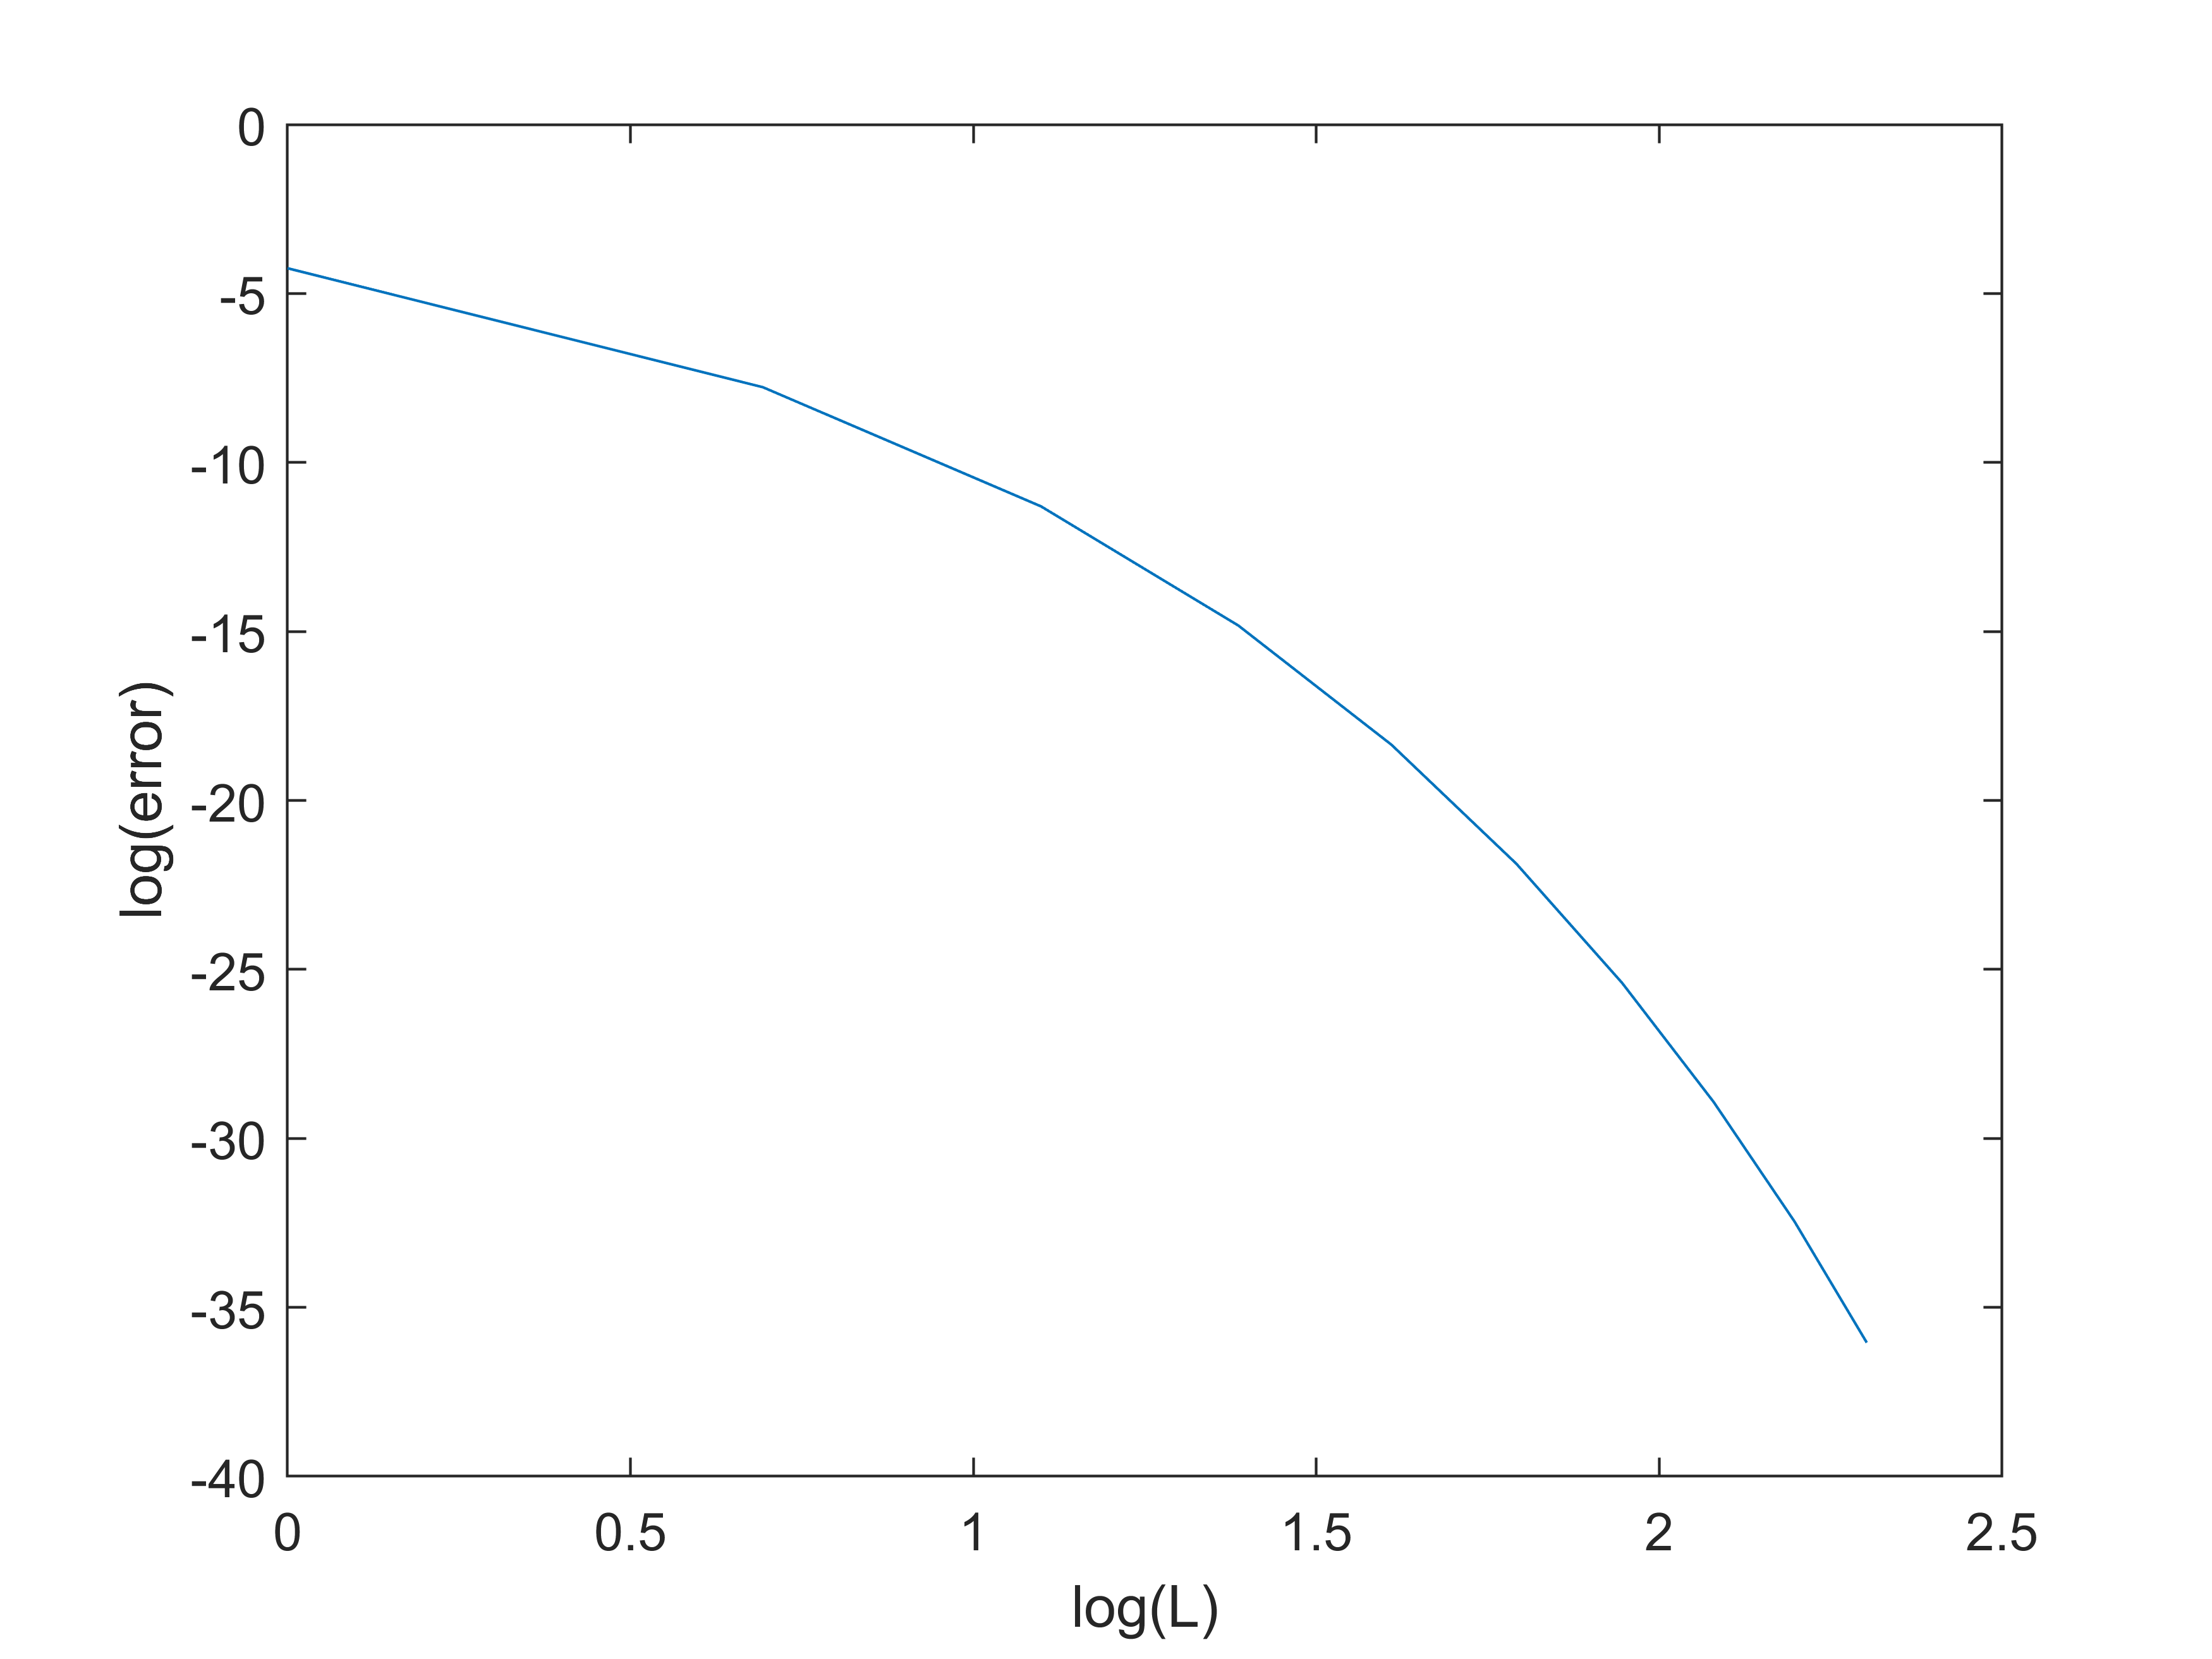
\includegraphics[width=\textwidth]{Files/q2,L=11.png}
            \caption{log-log plot of error against $L$ using numerical methods}
        \end{minipage}
        \hfill
    \begin{minipage}[b]{0.47\linewidth}
            \centering
            \textbf{Symbolic}\par
            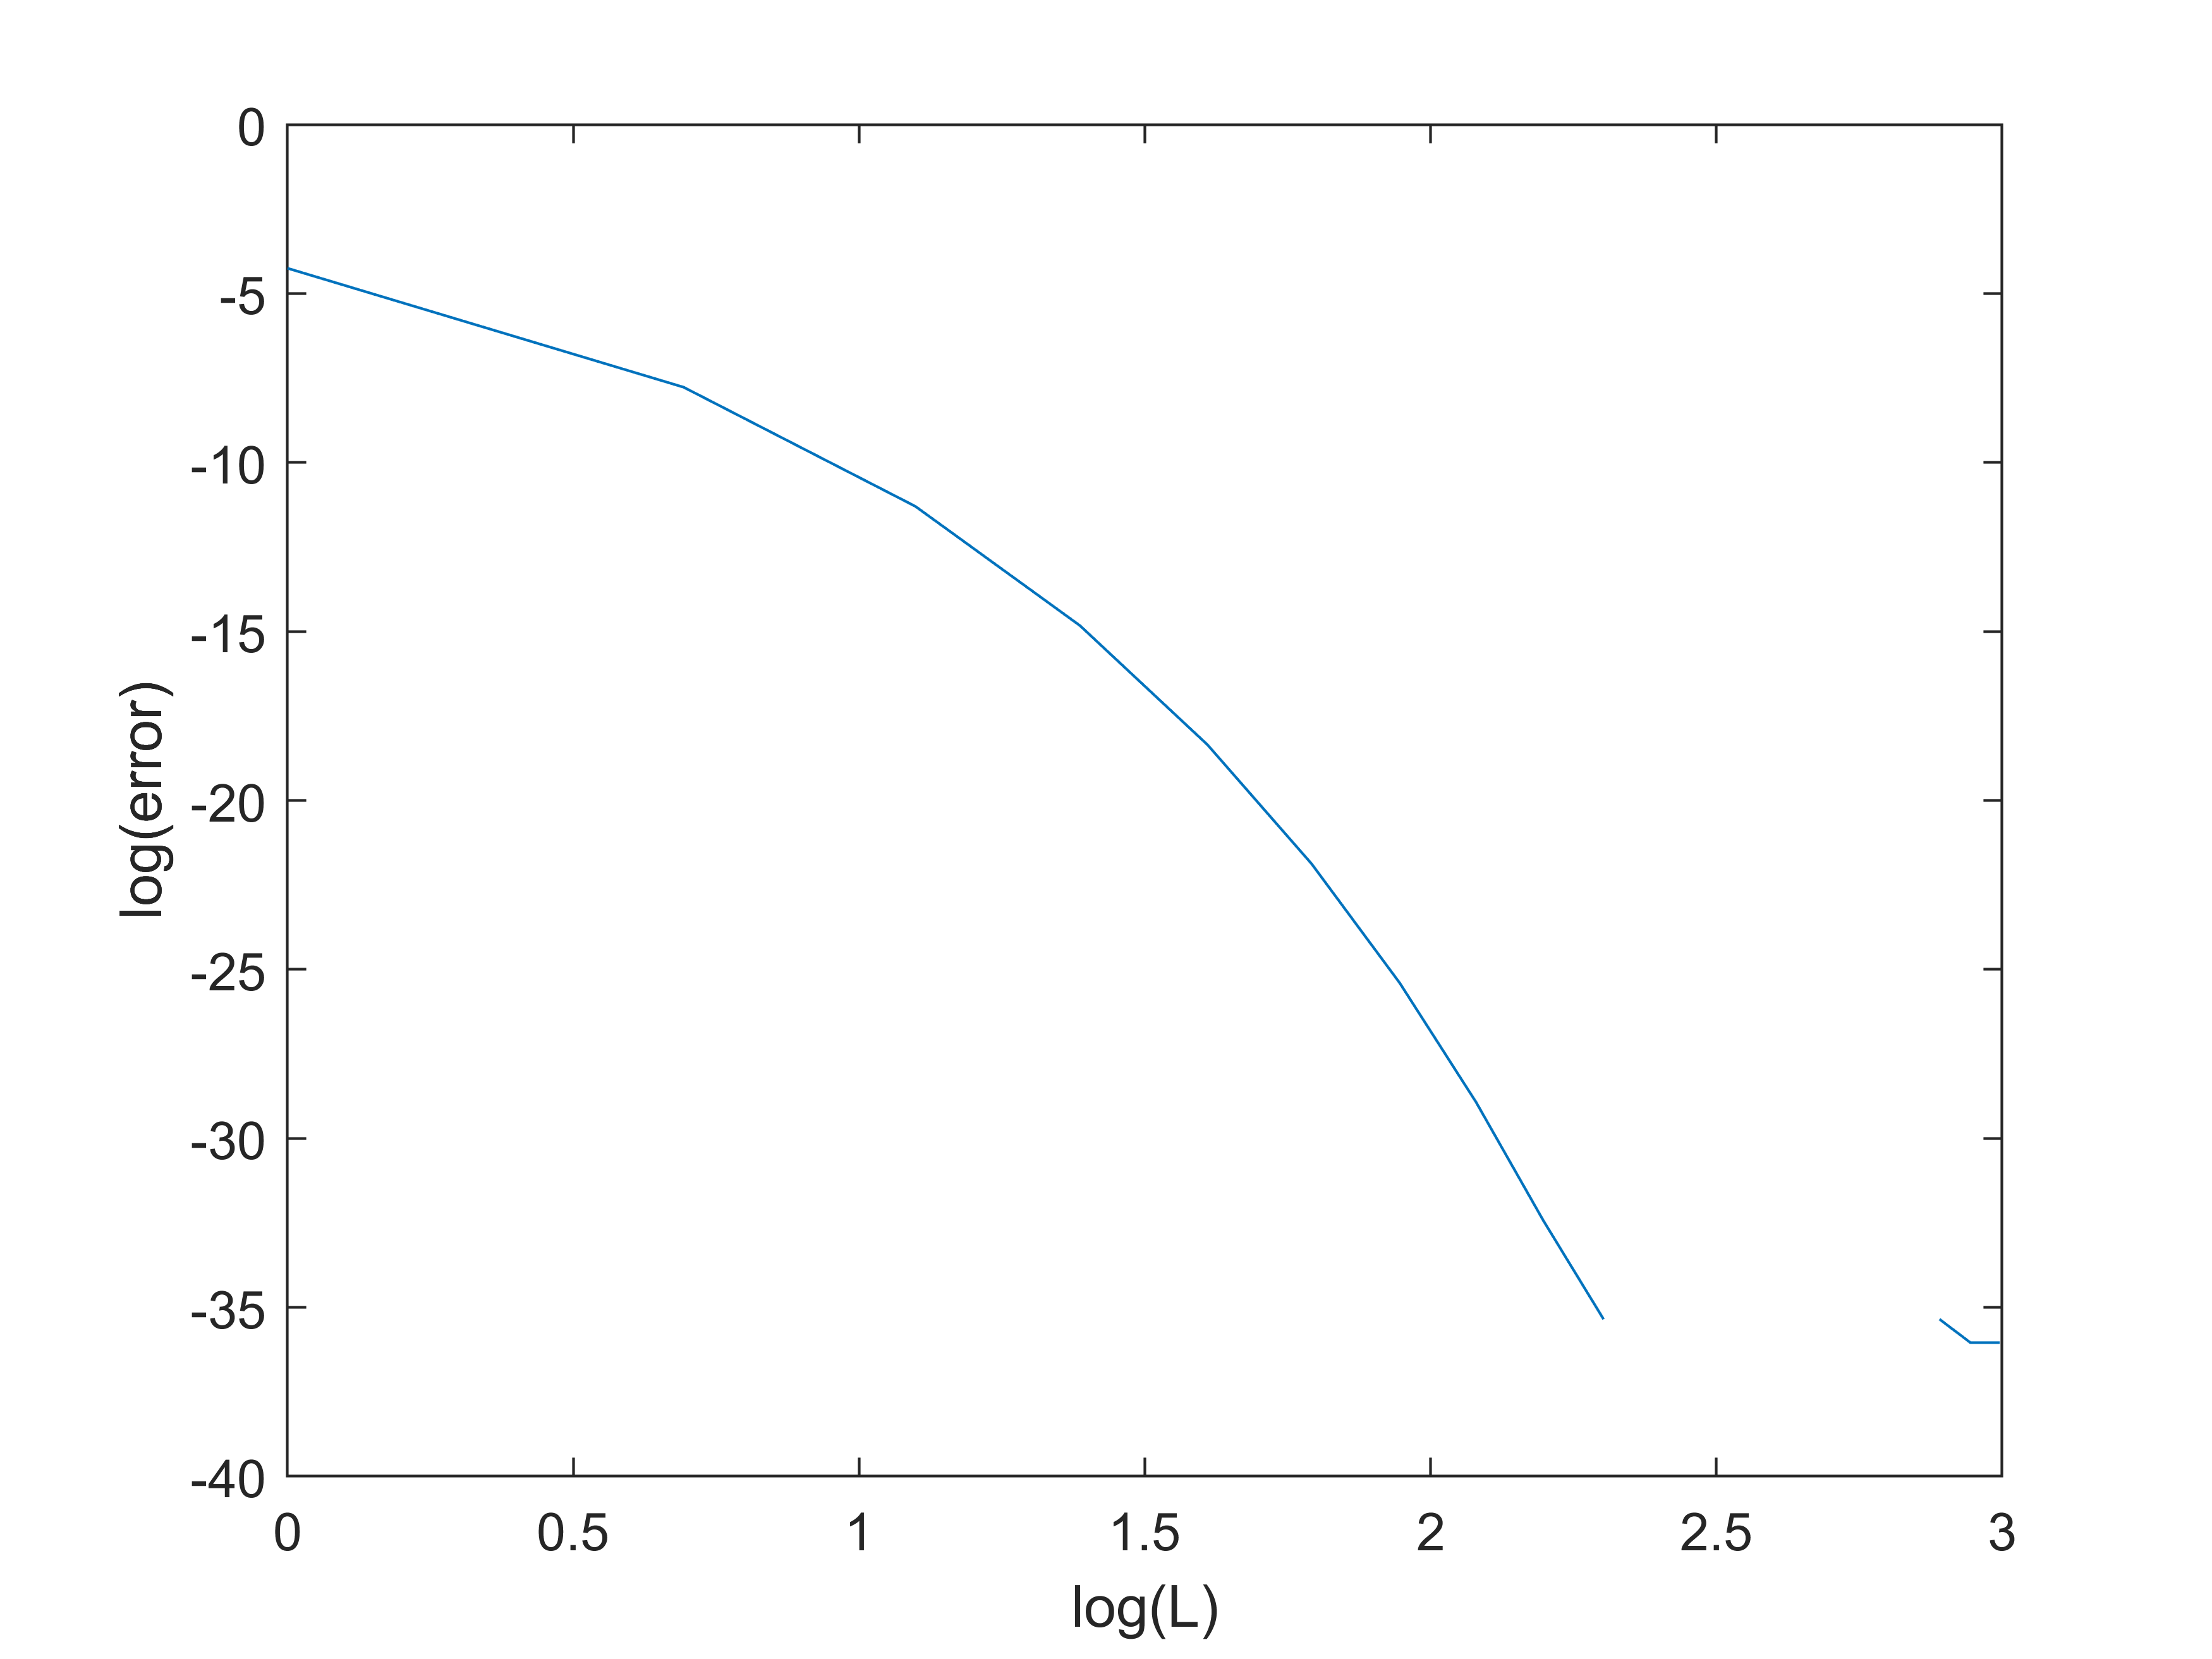
\includegraphics[width=\textwidth]{Files/q2,L=20.png}
            \caption{log-log plot of error against $L$ using symbolic calculation}
        \end{minipage}
\end{figure}
\noindent We can see from the graphs above, as $L$ increases, the error decreases and the rate of its decrease increases. We can see this as the gradient of the curve in the log-log plot is negative and the value of the gradient decreases as $\log L$ increases.\\
So we know the error decreases faster than $\mathcal{O}(L^k)$. Therefore, we plot $\log$(error) again $L$ to check if it's $\mathcal{O}(10^kL)$. If so, then we should have a straight line with gradient $k$ since $\log$(error(L))=$c+kL$.
\begin{figure}[H]
\centering
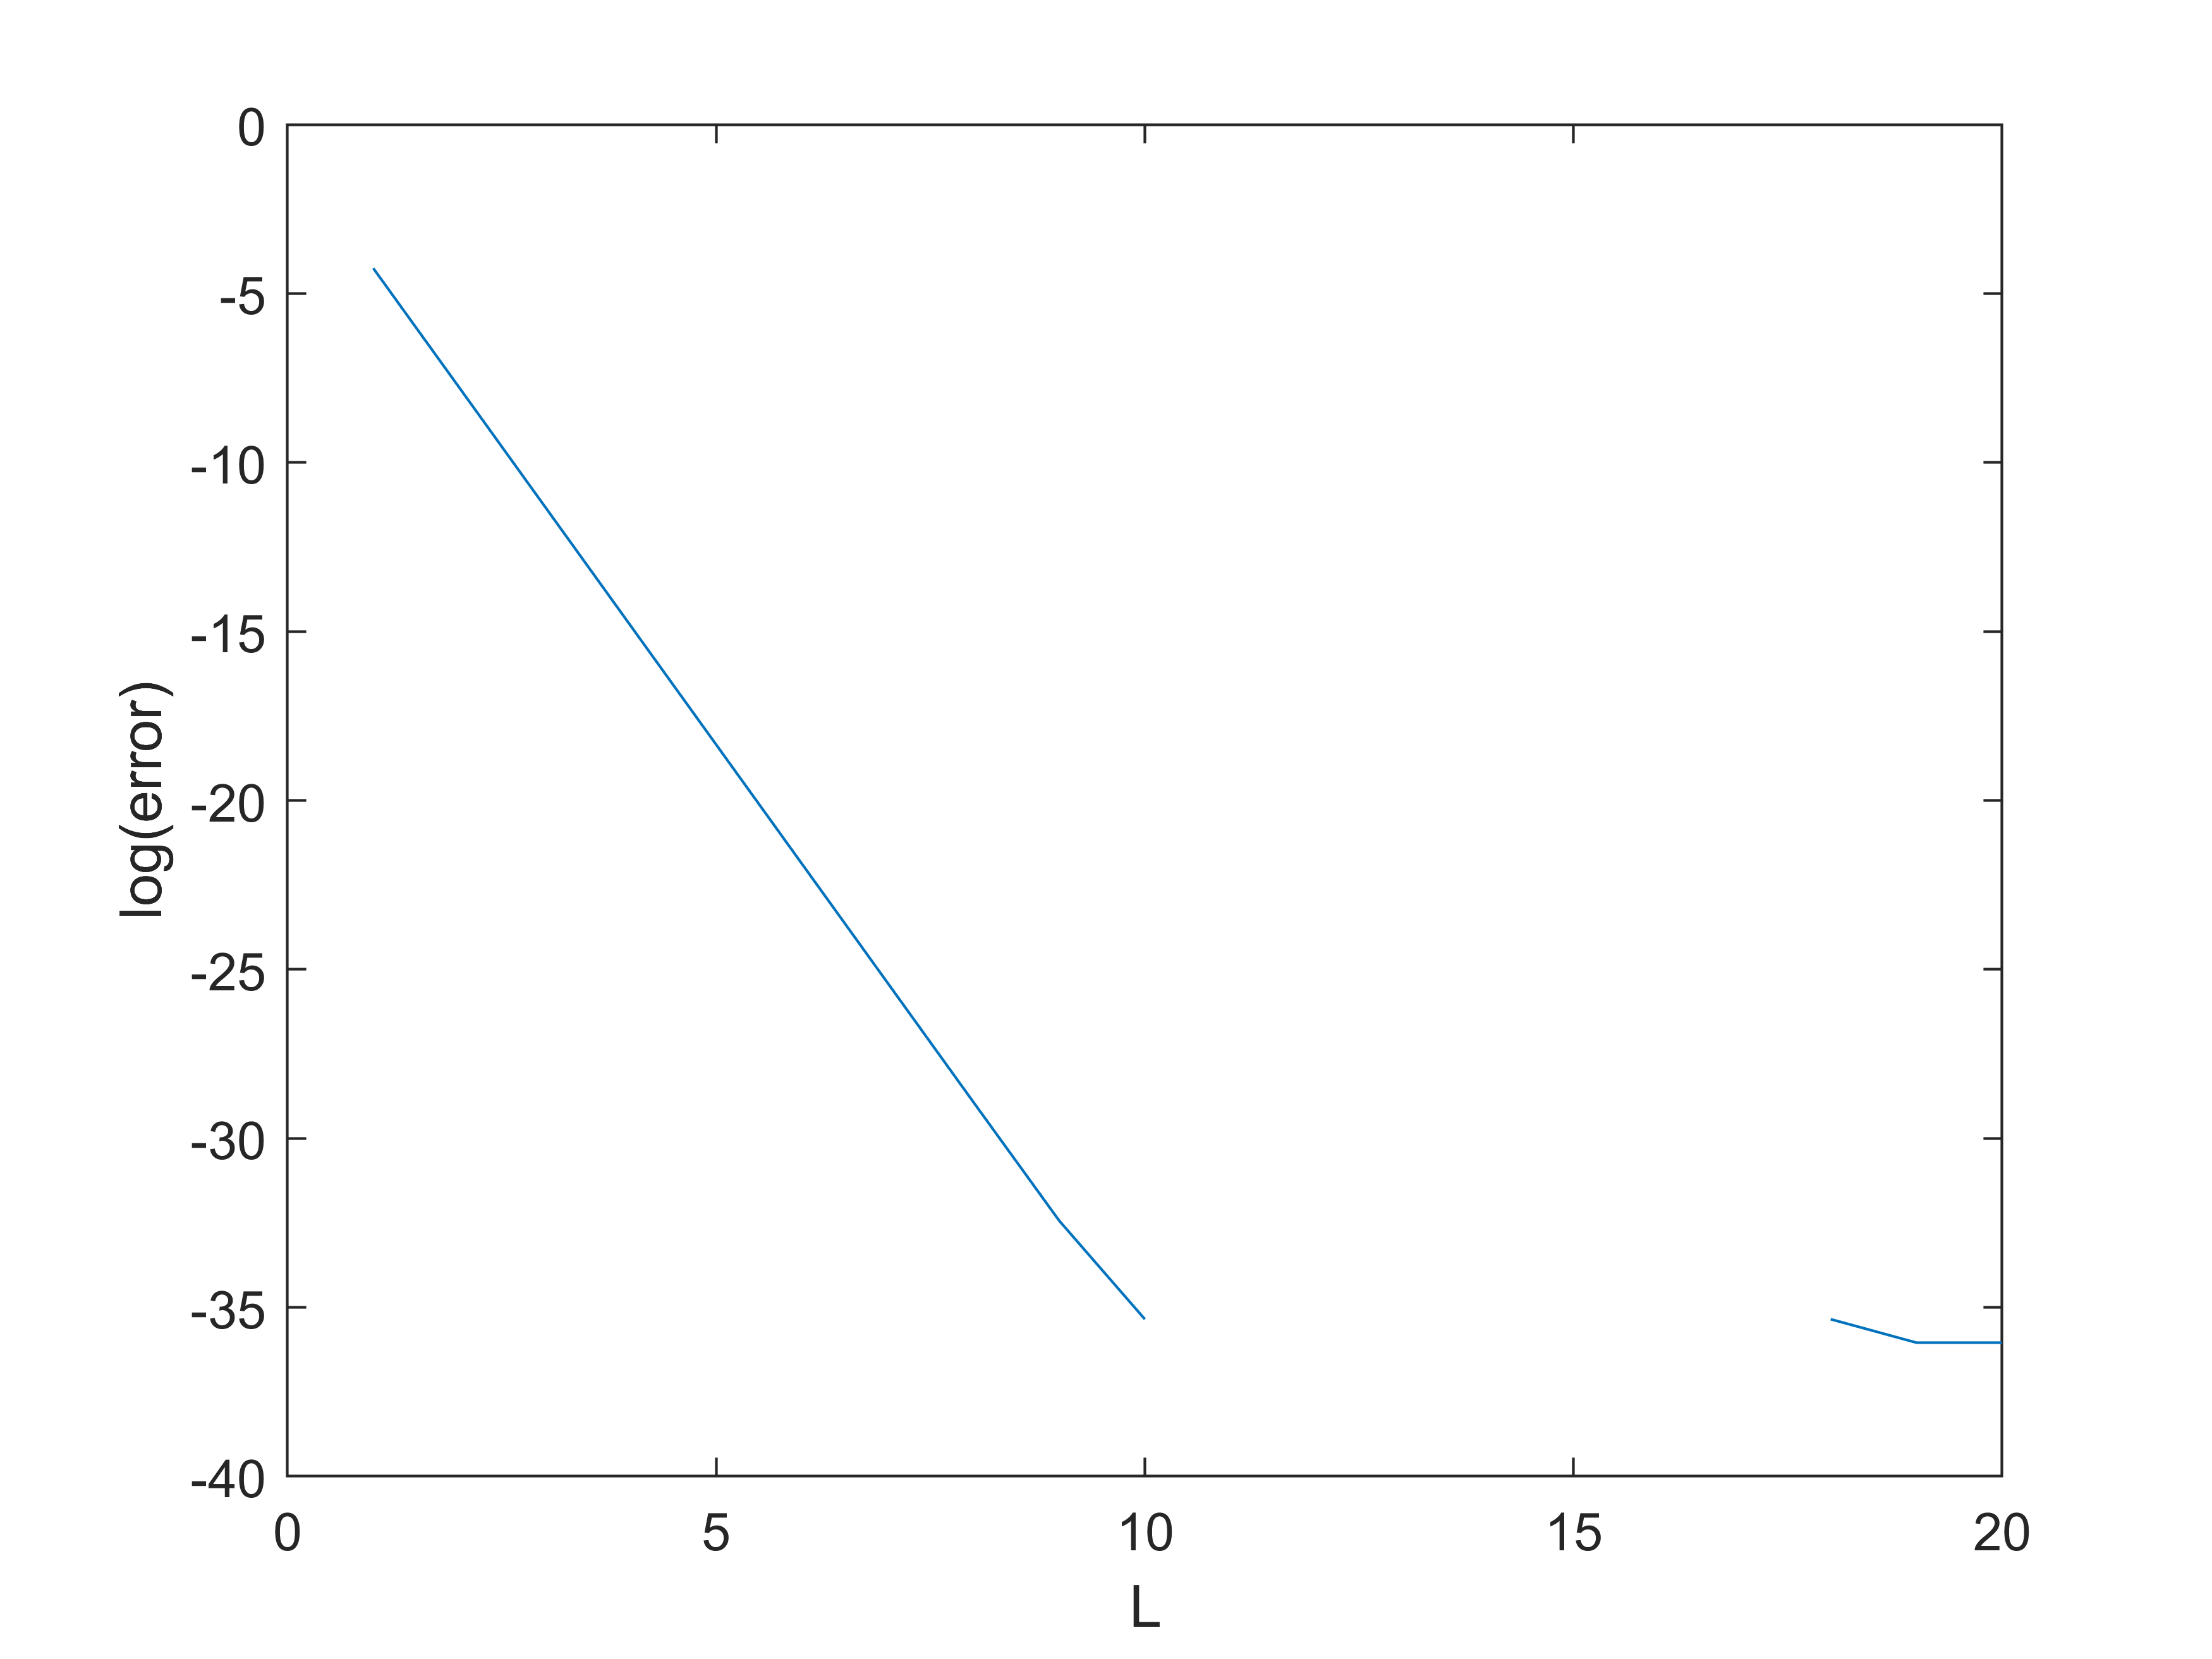
\includegraphics[width=0.47\textwidth]{Files/q2,L=20log.png}
\caption{Graph of $\log$(error) against $L$}
\end{figure}
\noindent This is indeed a straight line, and the gradient is roughly $-3.525$. So the error is roughly \underline{$\mathcal{O}(10^{\frac{-7L}{2}})$}.\\\\
Comparing the results for power series and for the Pade approximant, I would recommend using the Pade approximant to give an estimate for $\sqrt{2}$. The reason is that it converges to $\sqrt{2}$ much faster than the power series method, and allows us to find estimation of $\sqrt{2}$ to a very high specified accuracy before being restricted by computing power. If using power series method, the best we can do is error of size $10^{-5}$ whereas using Pade approximant method, we can get the error as low as $10^{-15}$.\\

\subsection*{Question 3}
We've found in question 1 that the radius of convergence for the power series method is $1$, when expanded about $x=0$. So the power series diverges for $x>1$. So the larger $N$ we use, the larger the error is for $1<x\leq100$. For fixed $N$, the larger $x$ is, the larger the error is.\\
In fact, the best approximation is to use $N=0,1$. We will plot these and $N=2$ on a separate graph. We do this using the program \emph{'v) q3\textunderscore power\textunderscore series.m'}.
\begin{figure}[H]
    \begin{minipage}[b]{0.47\linewidth}
            \centering
            \textbf{Power Series, N=0,1}\par
            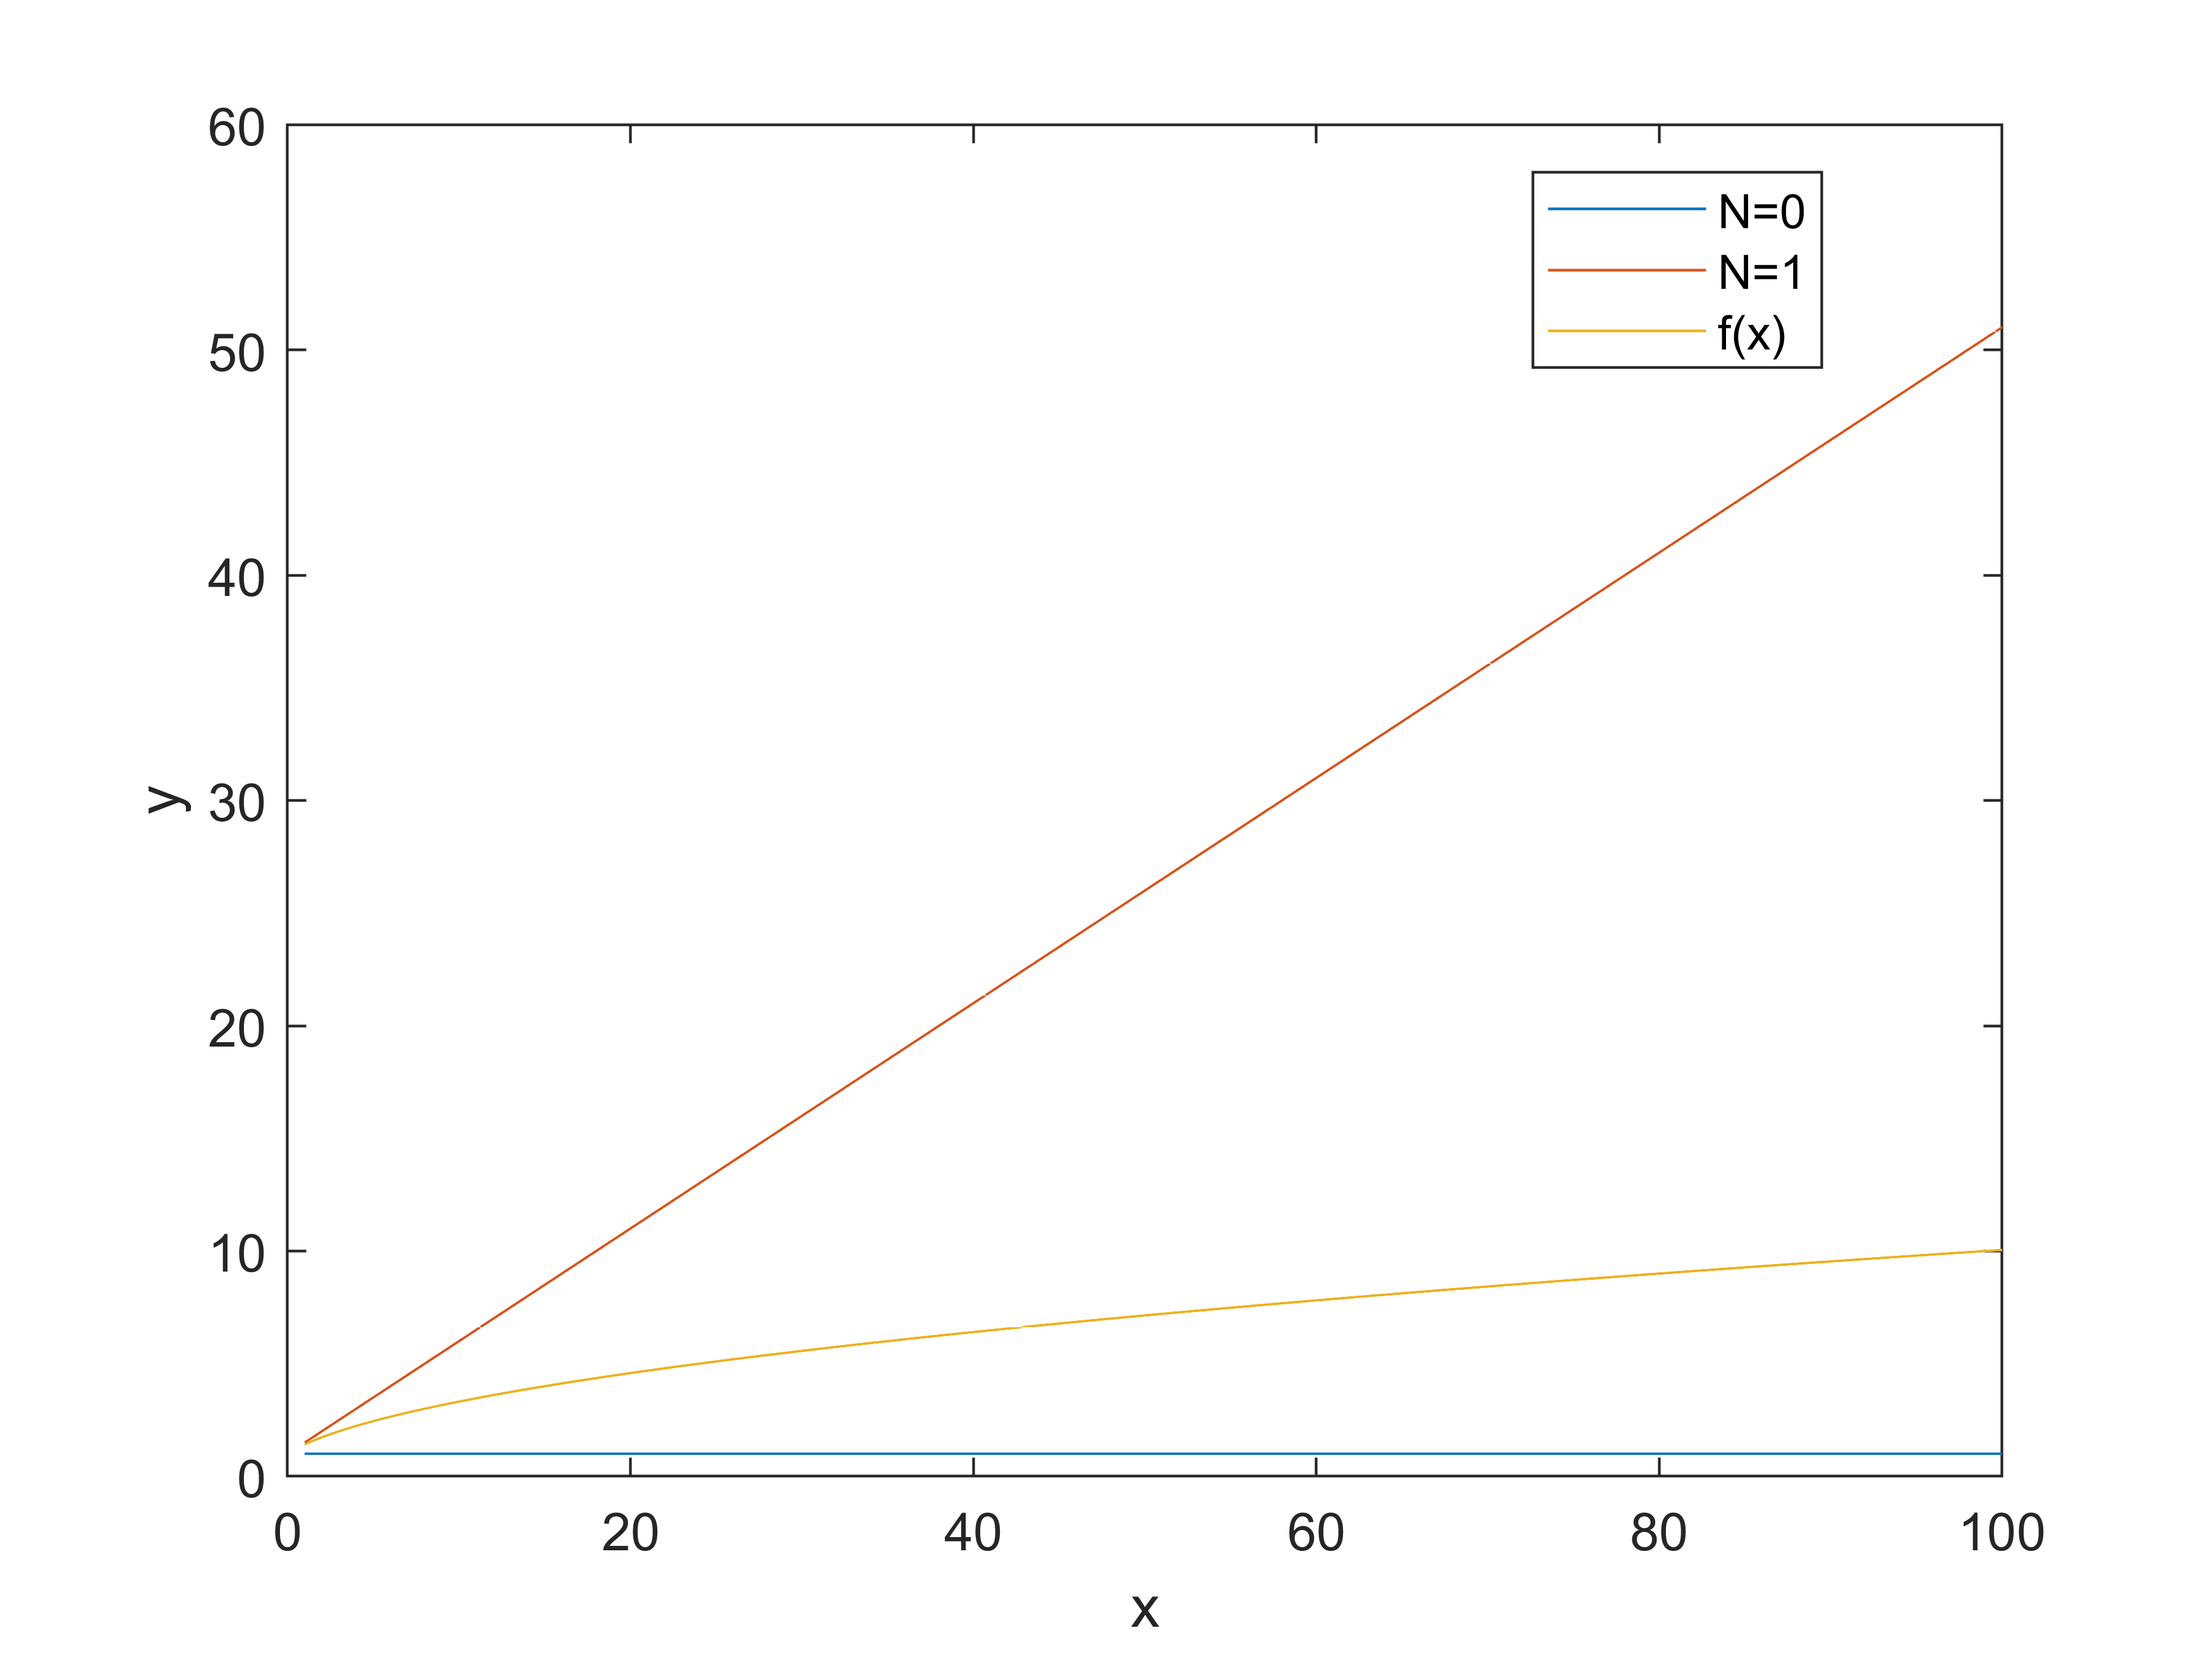
\includegraphics[width=\textwidth]{Files/q3_ps,N=0,1.png}
            \caption{Graph of power series approximation of $f_1(x)$ against $x$ for $x\in(1,100],N=\{0,1\}$}
        \end{minipage}
        \hfill
    \begin{minipage}[b]{0.47\linewidth}
            \centering
            \textbf{Power Series, N=2,3}\par
            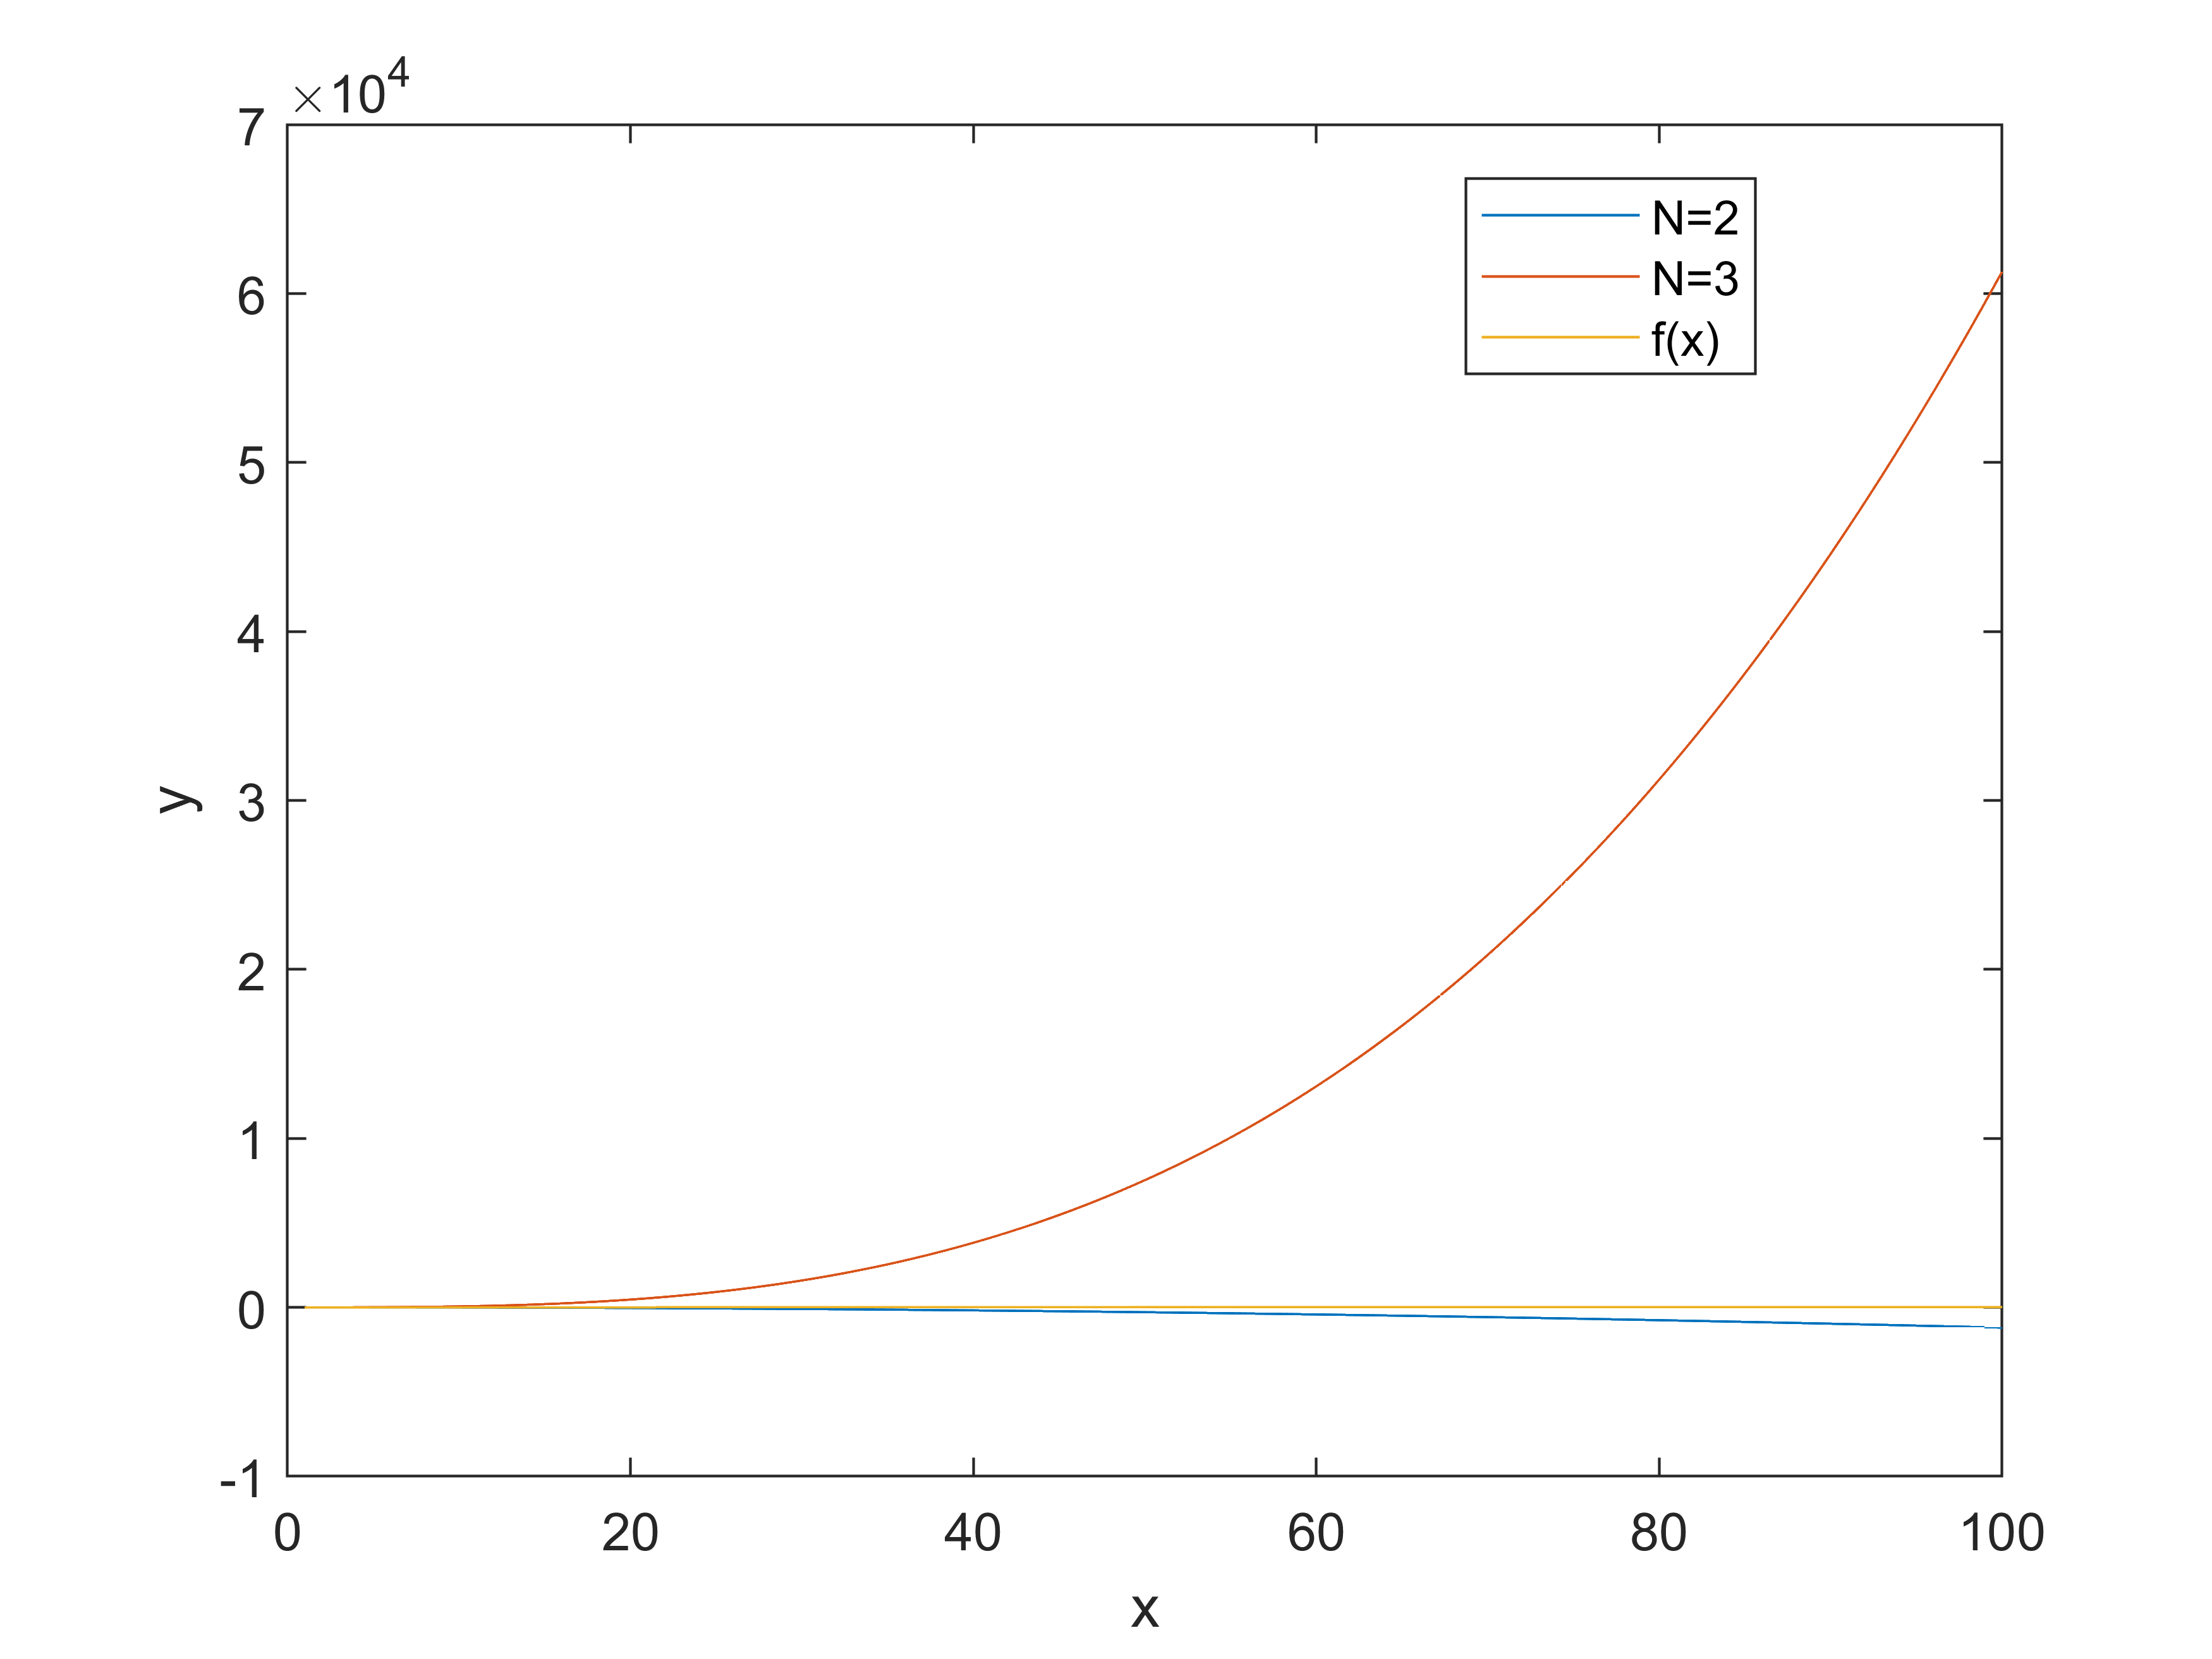
\includegraphics[width=\textwidth]{Files/q3_ps,N=2,3.png}
            \caption{Graph of power series approximation of $f_1(x)$ against $x$ for $x\in(1,100],N=\{2,3\}$}
        \end{minipage}
\end{figure}
\noindent We can see in the graphs that the best approximation using the power series method is the straight line $y=1$ at $N=0$. This is because for $x>>1$, the dominant term of the N-truncated power series is $c_Nx^N$, which is much larger than $f_1(x)$ which has leading order $x^{\frac{1}{2}}$.\\
The sign of the approximation will switch between $N$ and $N+1$. This is because $C_N$ is negative for $N$ even and positive for $N$ odd. The magnitude of the approximation will also be about $\frac{C_{N+1}}{C_N}x$ times larger at $x>>1$ when $N$ is increased by 1. \\
Subbing in the values for $C_{N+1}$ and $C_N$, we find $\frac{C_{N+1}}{C_N}x=\frac{2N-1}{2(N+1)}x\approx x$, for $N$ sufficiently large.\\\\
\noindent For Pade approximants, we plot the estimates using the program \emph{'vii) q3\textunderscore pade.m'}. In this program, we used a new function \emph{'vi) CoefPade.m'}, but this is really the same as \emph{'i) CoefSolver.m'}, the only difference is that \textit{'CoefPade.m'} outputs the coefficients $p,q$ instead of the evaluation at some point $y$.\\
We do this with $L=1,3,5,10$.
\begin{figure}[H]
\centering
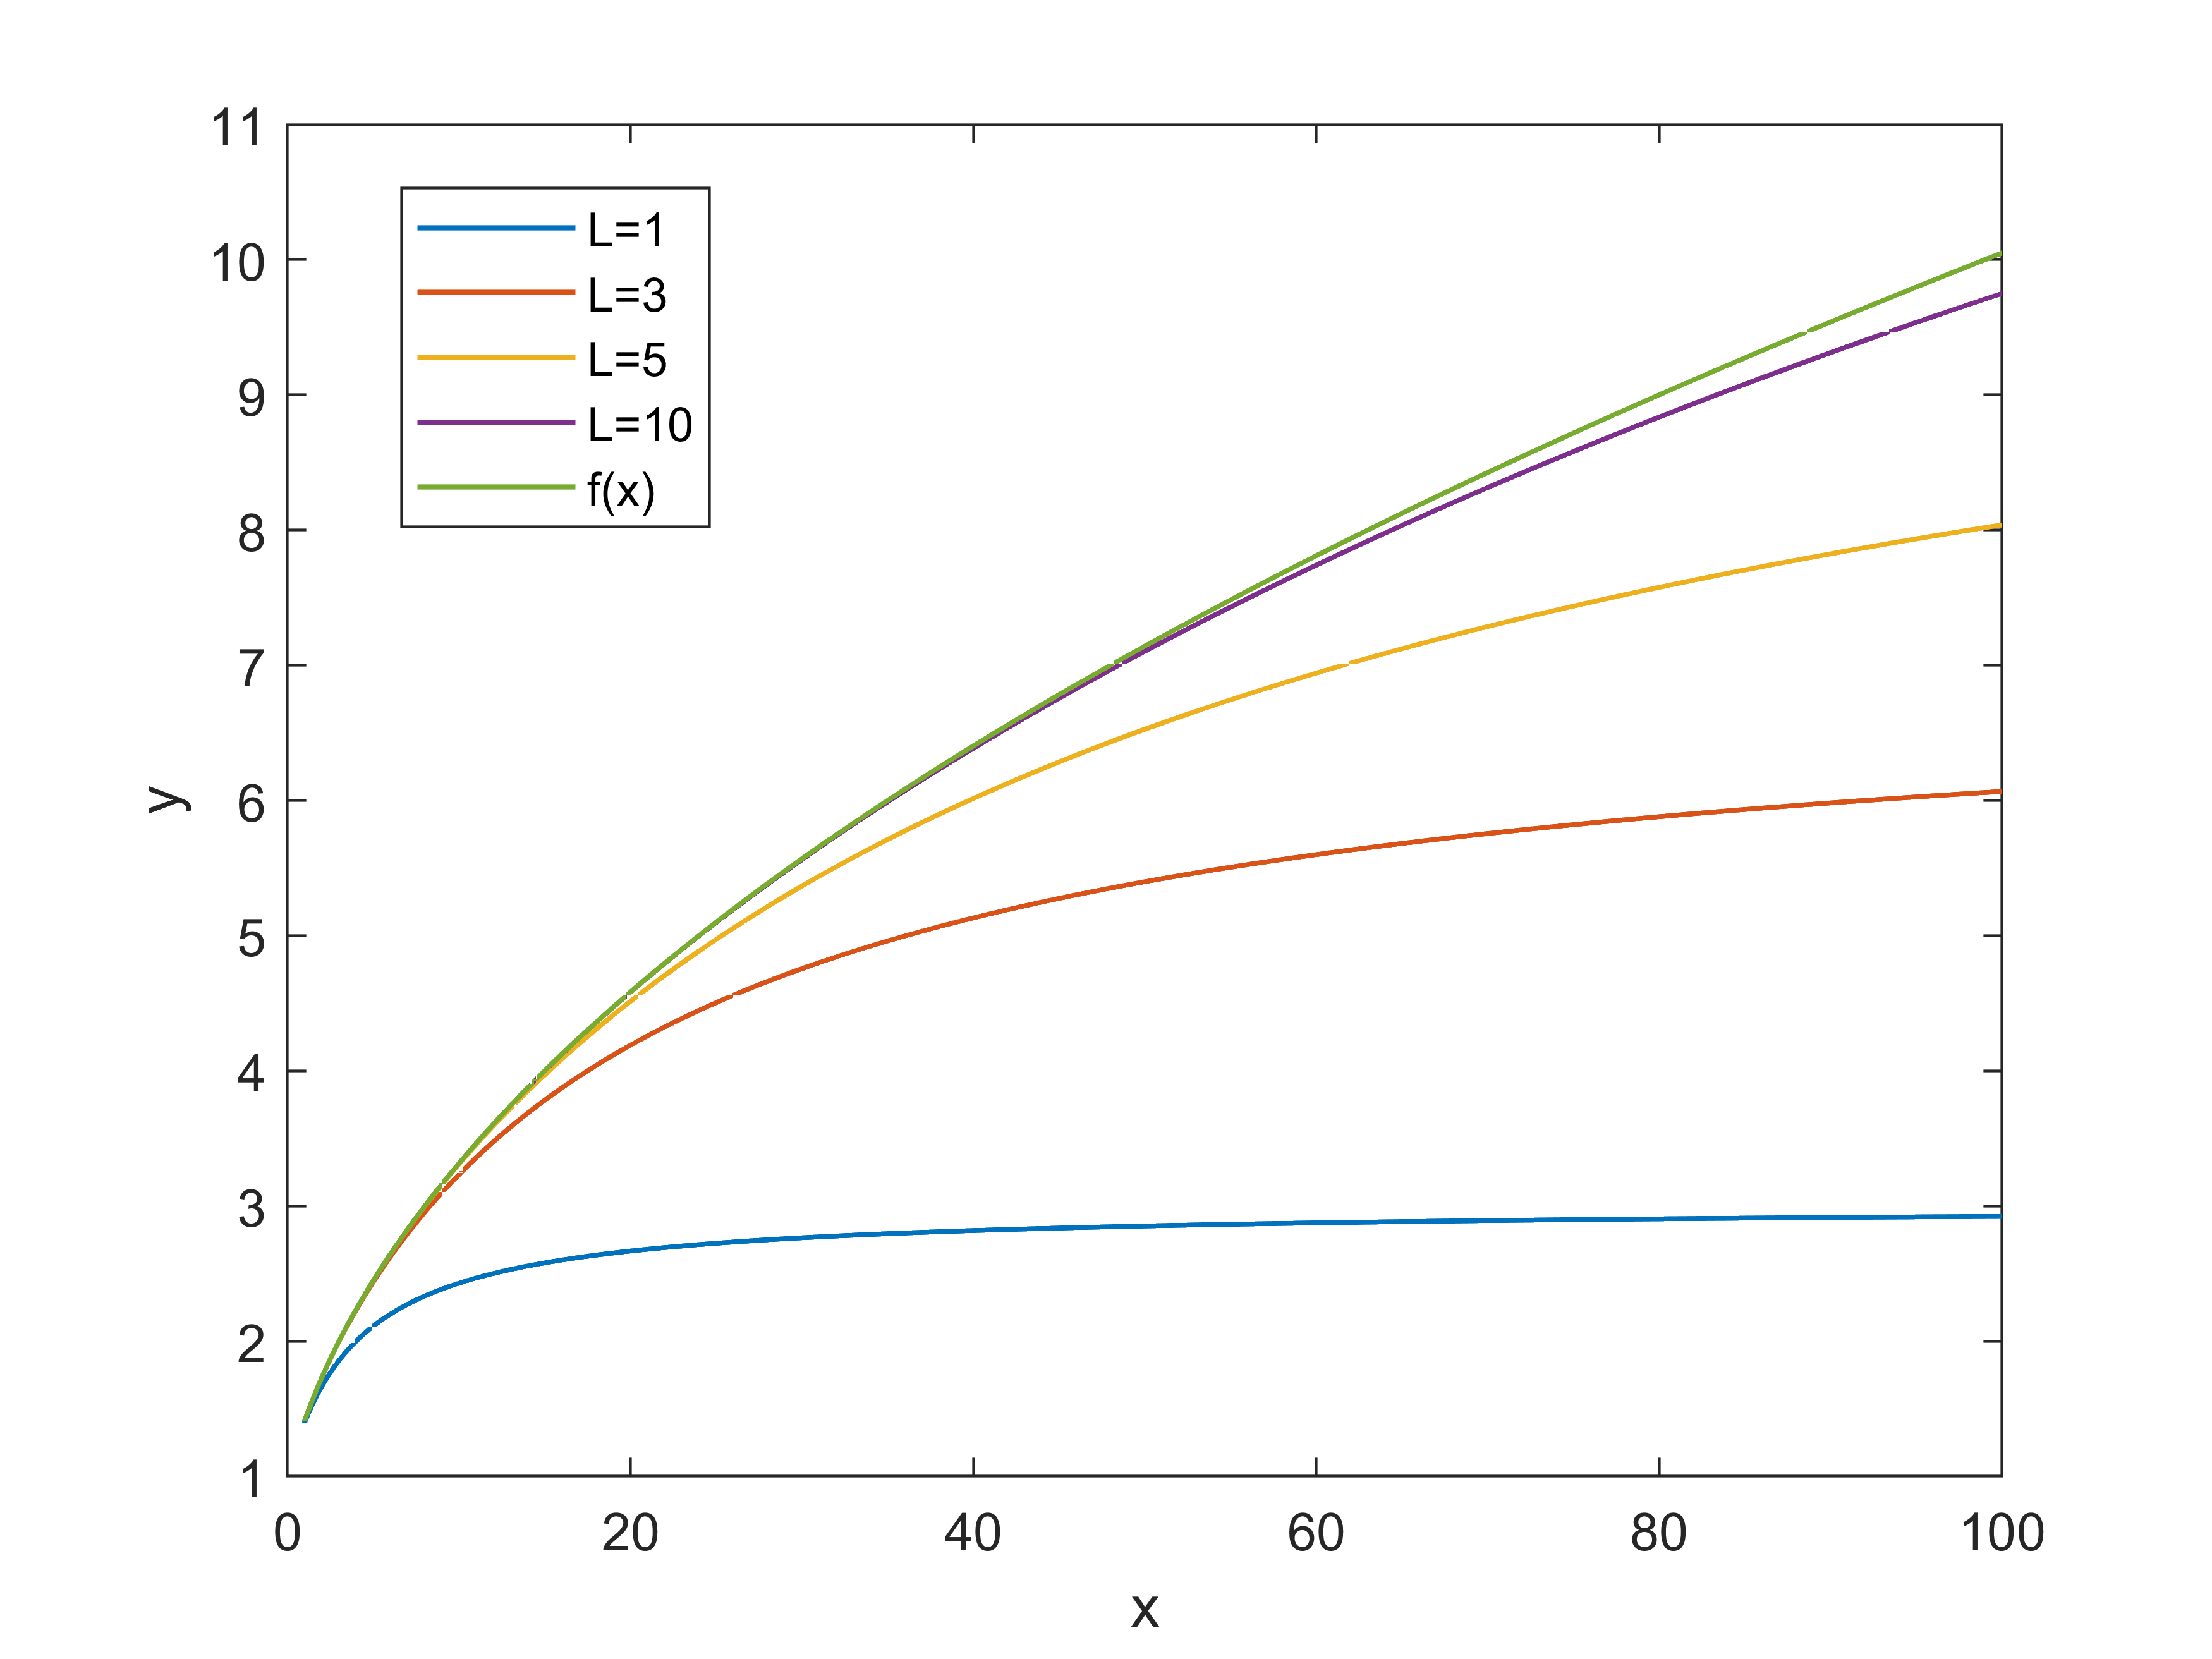
\includegraphics[width=0.5\textwidth]{Files/q3,pade.png}
\caption{Graph of Pade approximant Estimate of $f_1(x)$ against $x$ for $x\in(1,100],L=\{1,3,5,10\}$}
\end{figure}
\noindent We note that the Pade approximant estimates are always smaller in value compared to $f_1(x)$, and as $L$ increases, the estimates converges to $f_1(x)$ from below $f_1(x)$ for all $x\in(1,100]$. \\
We also note that the error is dependent of $x$, for example the error of the $L=3$ estimate to $f_1(x)$ for $x<5$ is less than $0.01$ whereas for $x>50$, the error is larger than $1.5$.\\
\begin{figure}[H]
    \begin{minipage}[b]{0.47\linewidth}
            \centering
            \textbf{x=10}\par
            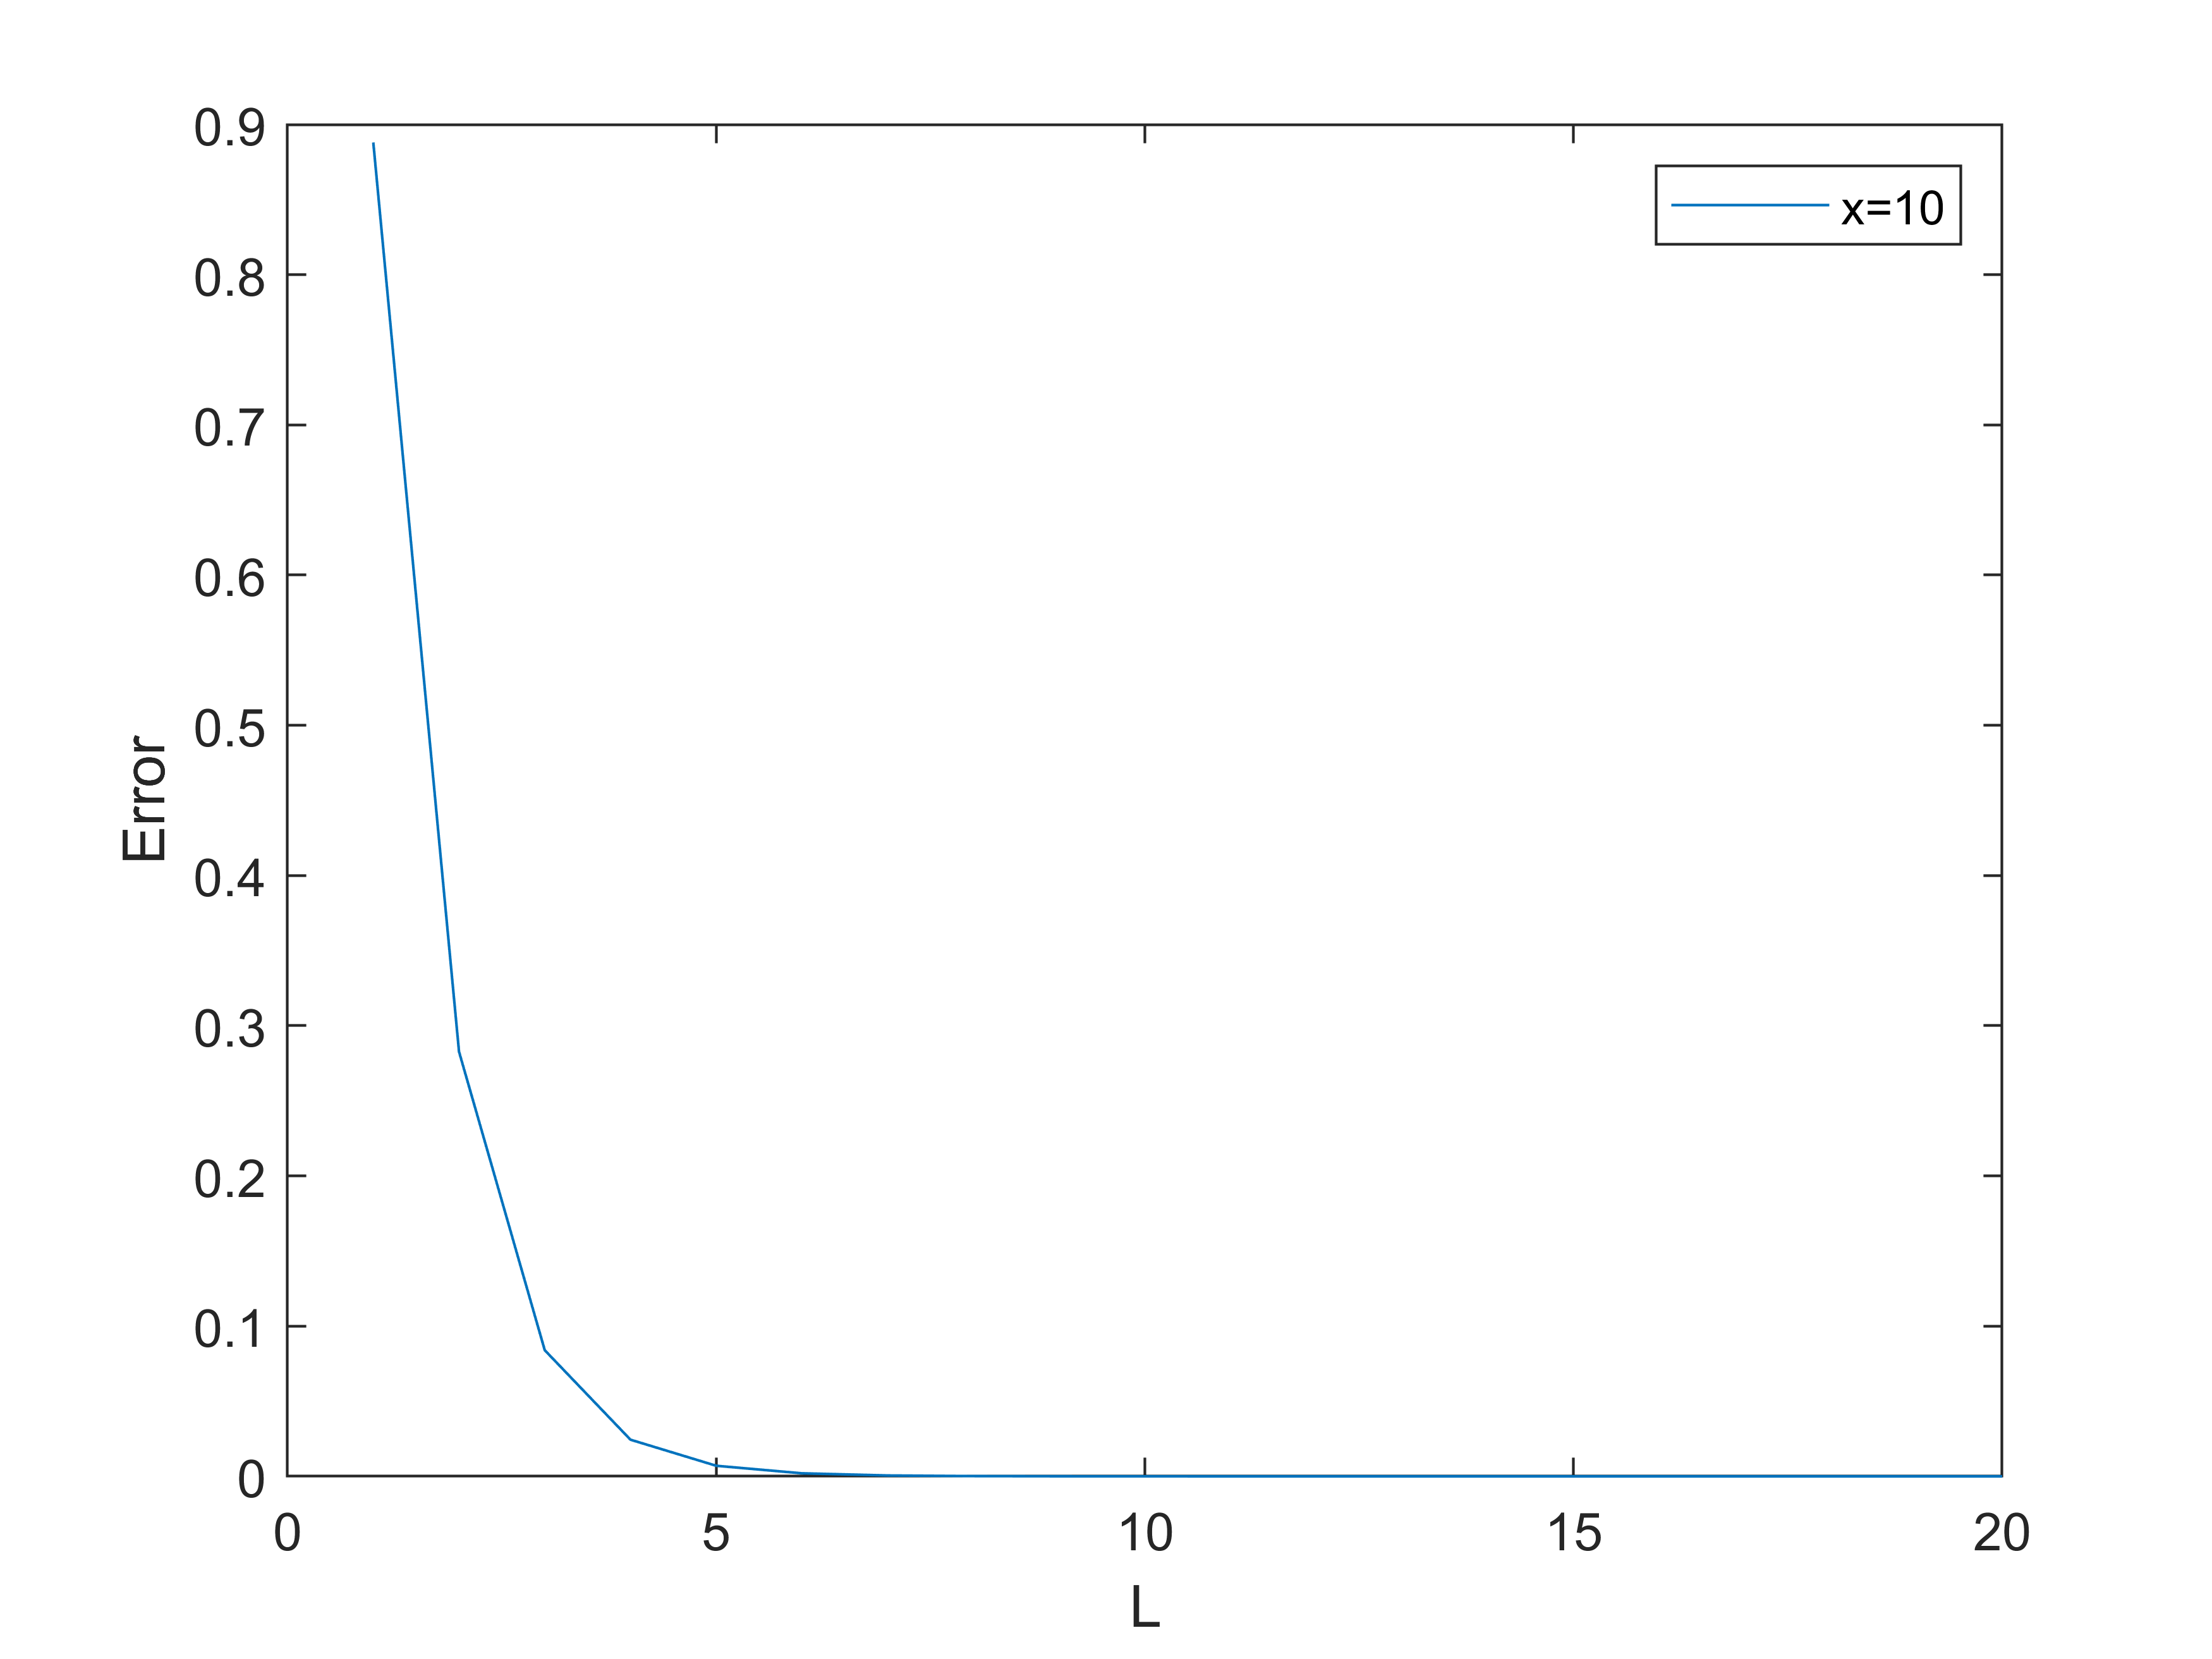
\includegraphics[width=\textwidth]{Files/q3_pp_10.png}
            \caption{Graph of Pade approximant error against $L$ at $x=10$}
        \end{minipage}
        \hfill
    \begin{minipage}[b]{0.47\linewidth}
            \centering
            \textbf{x=100}\par
            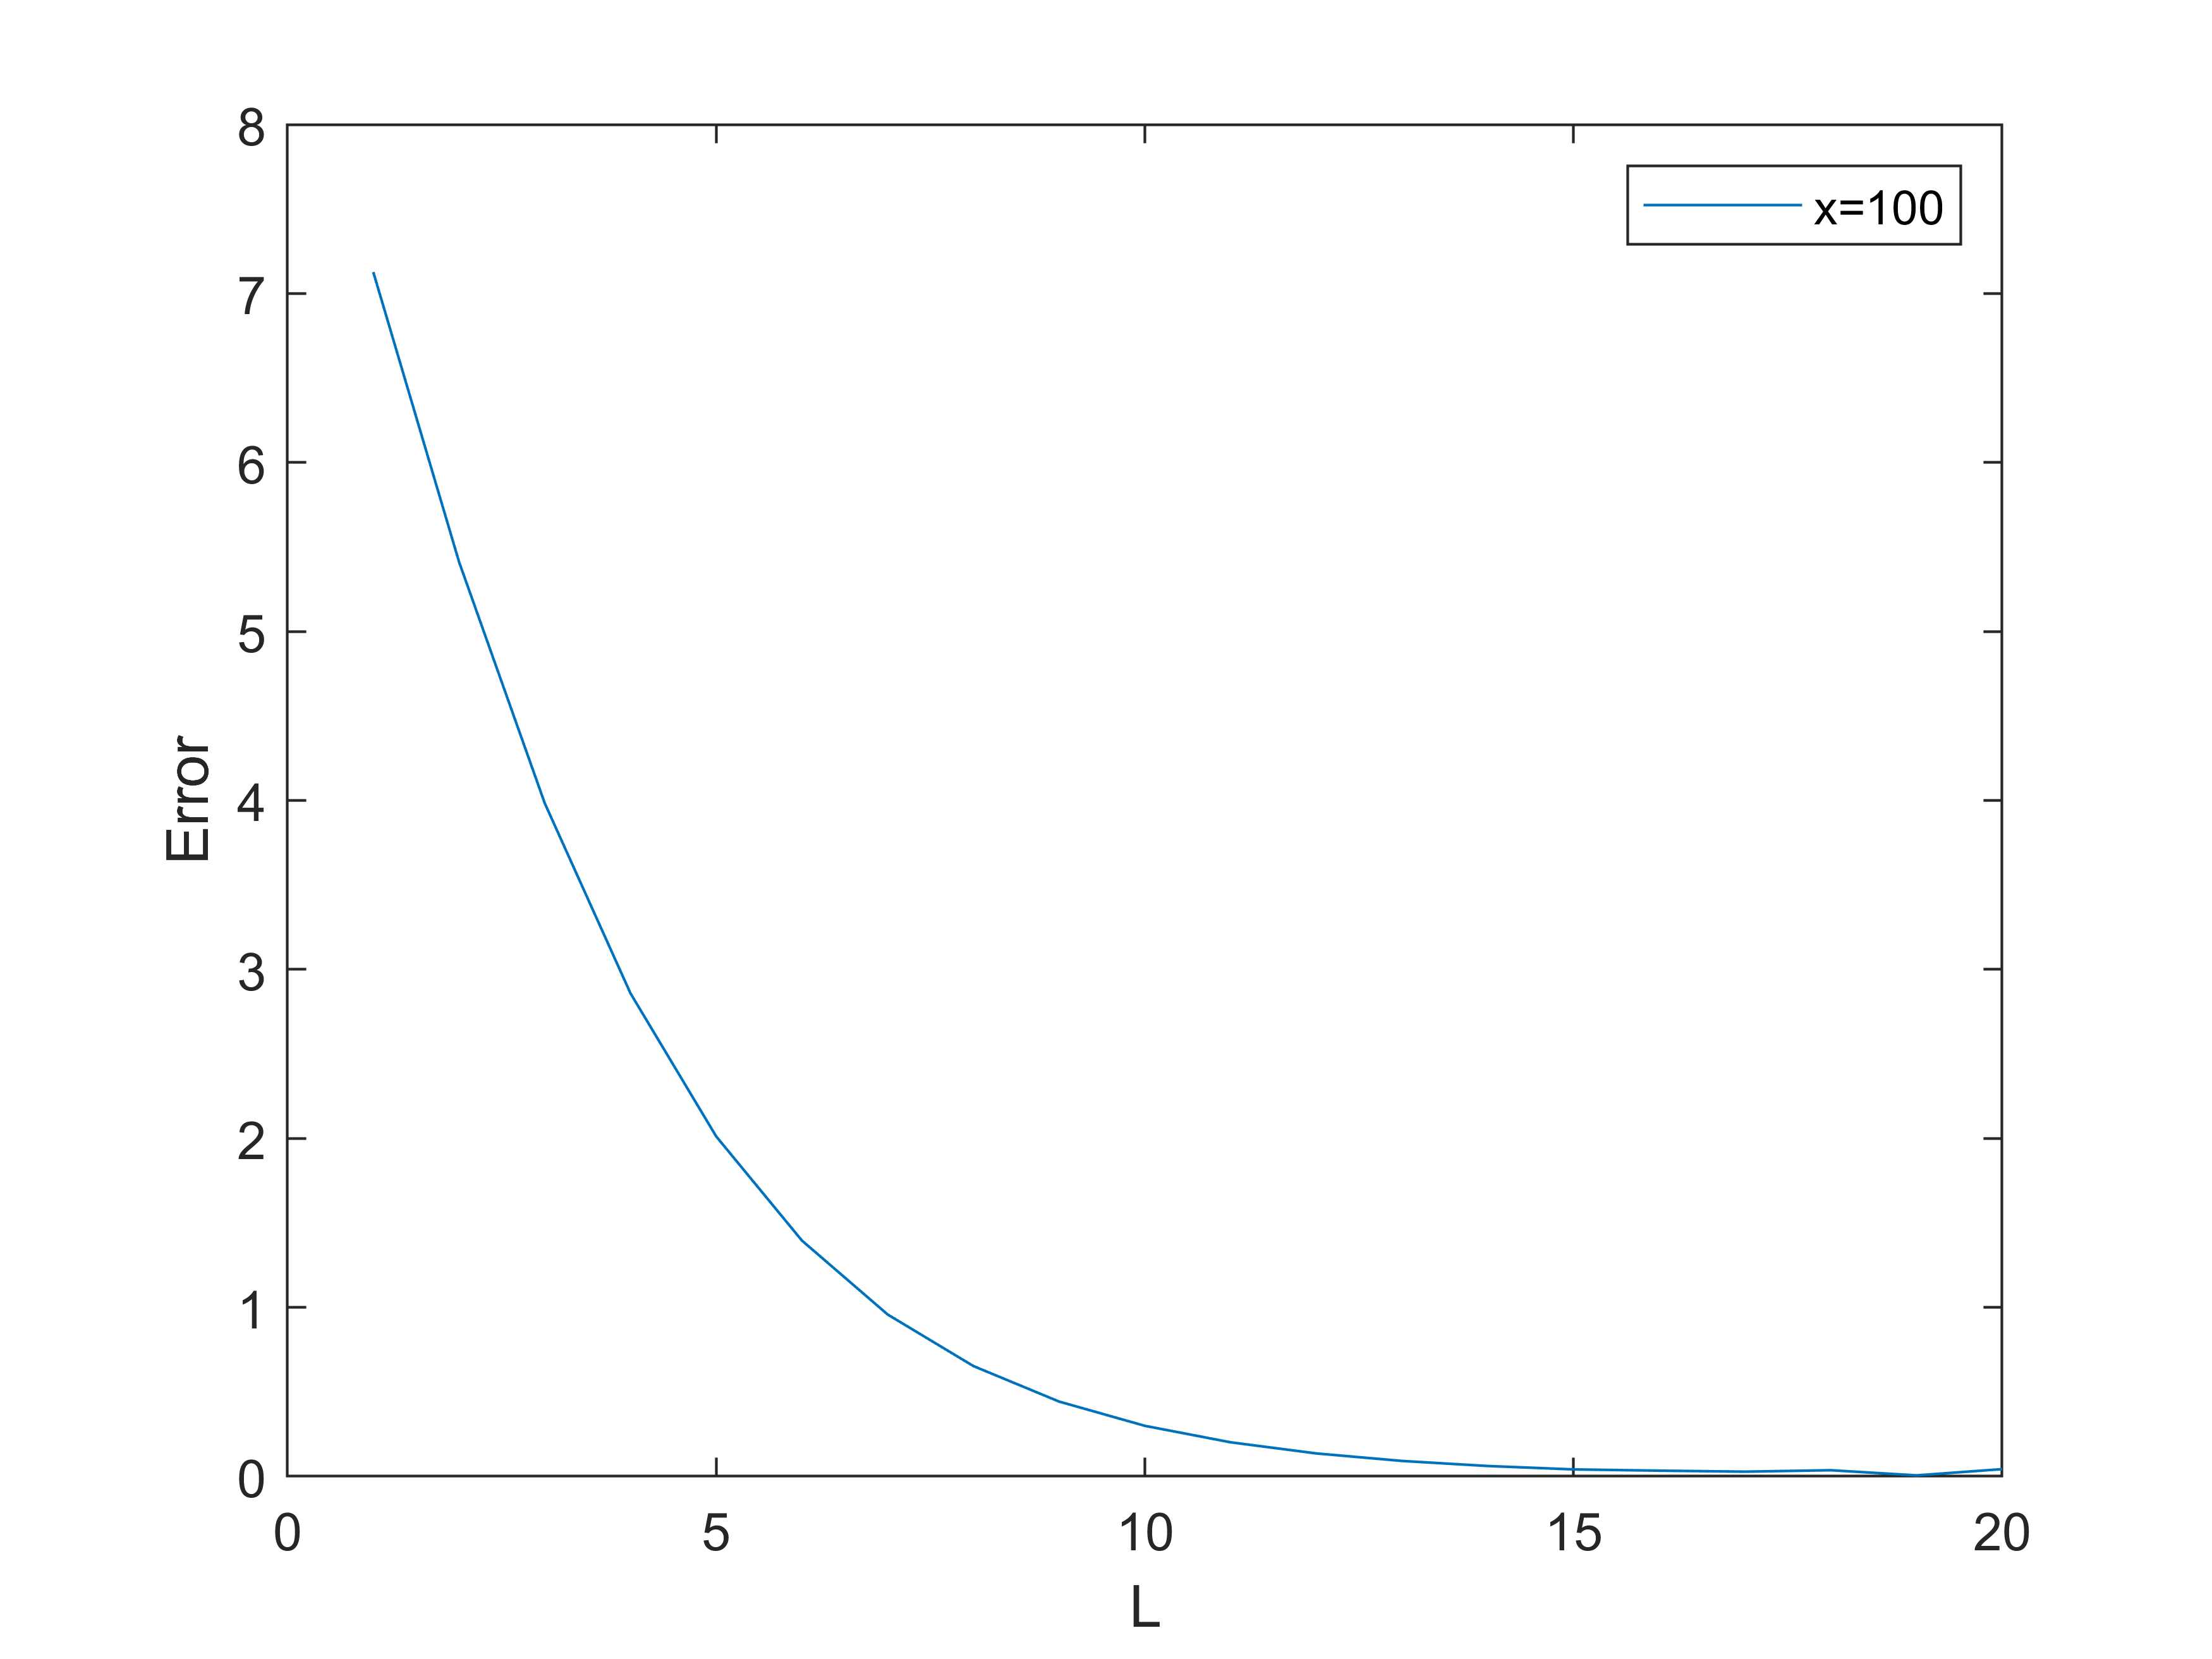
\includegraphics[width=\textwidth]{Files/q3_pp_100.png}
            \caption{Graph of Pade approximant error against $L$ at $x=100$}
        \end{minipage}
\end{figure}
\noindent We will further investigate how the error in Pade approximant varies as $L$ increases at $x=10,100$.\\
We do this using the program \emph{'viii) q3\textunderscore pade\textunderscore points.m'}.\\
We first plot the error against $L$ directly at both $x=10$ and $x=100$, we note that the plotted line looks like it follows an exponential relationship $10^{-k(x)L}$ with $L$ when $x$ is fixed. We therefore plot $\log(error)$ against $L$ for $x=10,100$.\\
\begin{figure}[H]
    \begin{minipage}[b]{0.47\linewidth}
            \centering
            \textbf{x=10}\par
            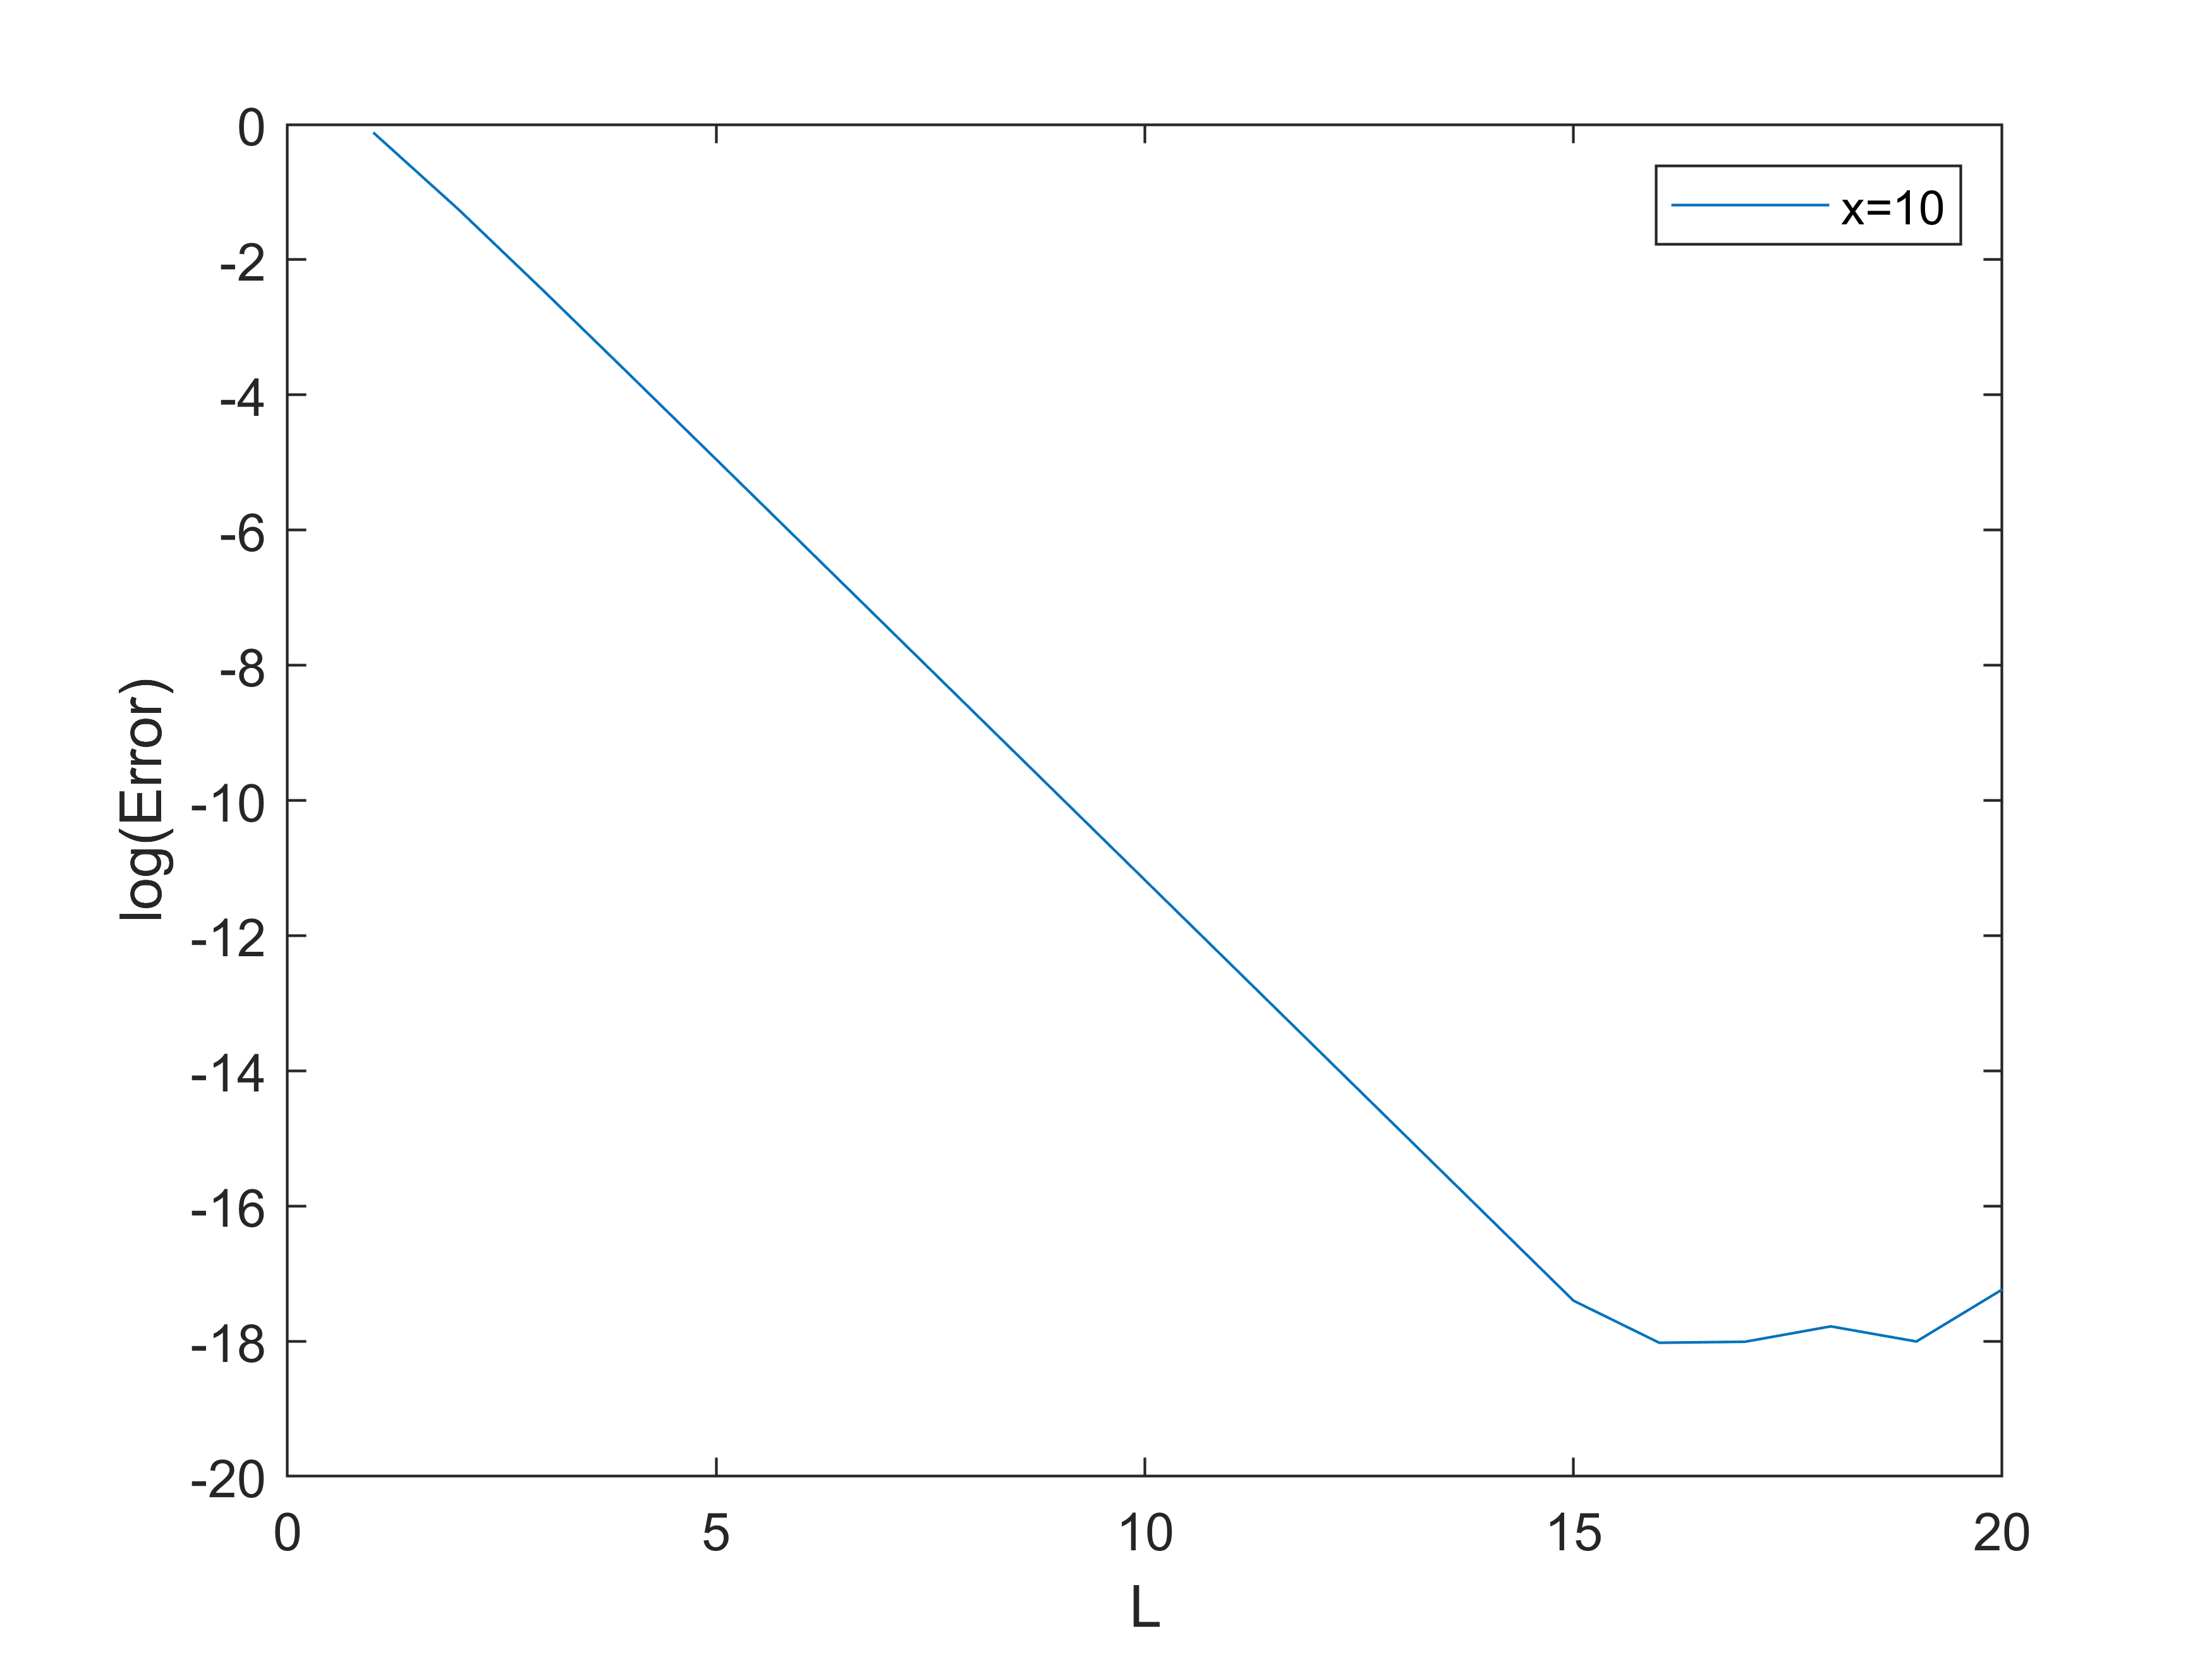
\includegraphics[width=\textwidth]{Files/q3_pp_10_log.png}
            \caption{Graph of Pade approximant error against $L$ at $x=10$}
        \end{minipage}
        \hfill
    \begin{minipage}[b]{0.47\linewidth}
            \centering
            \textbf{x=100}\par
            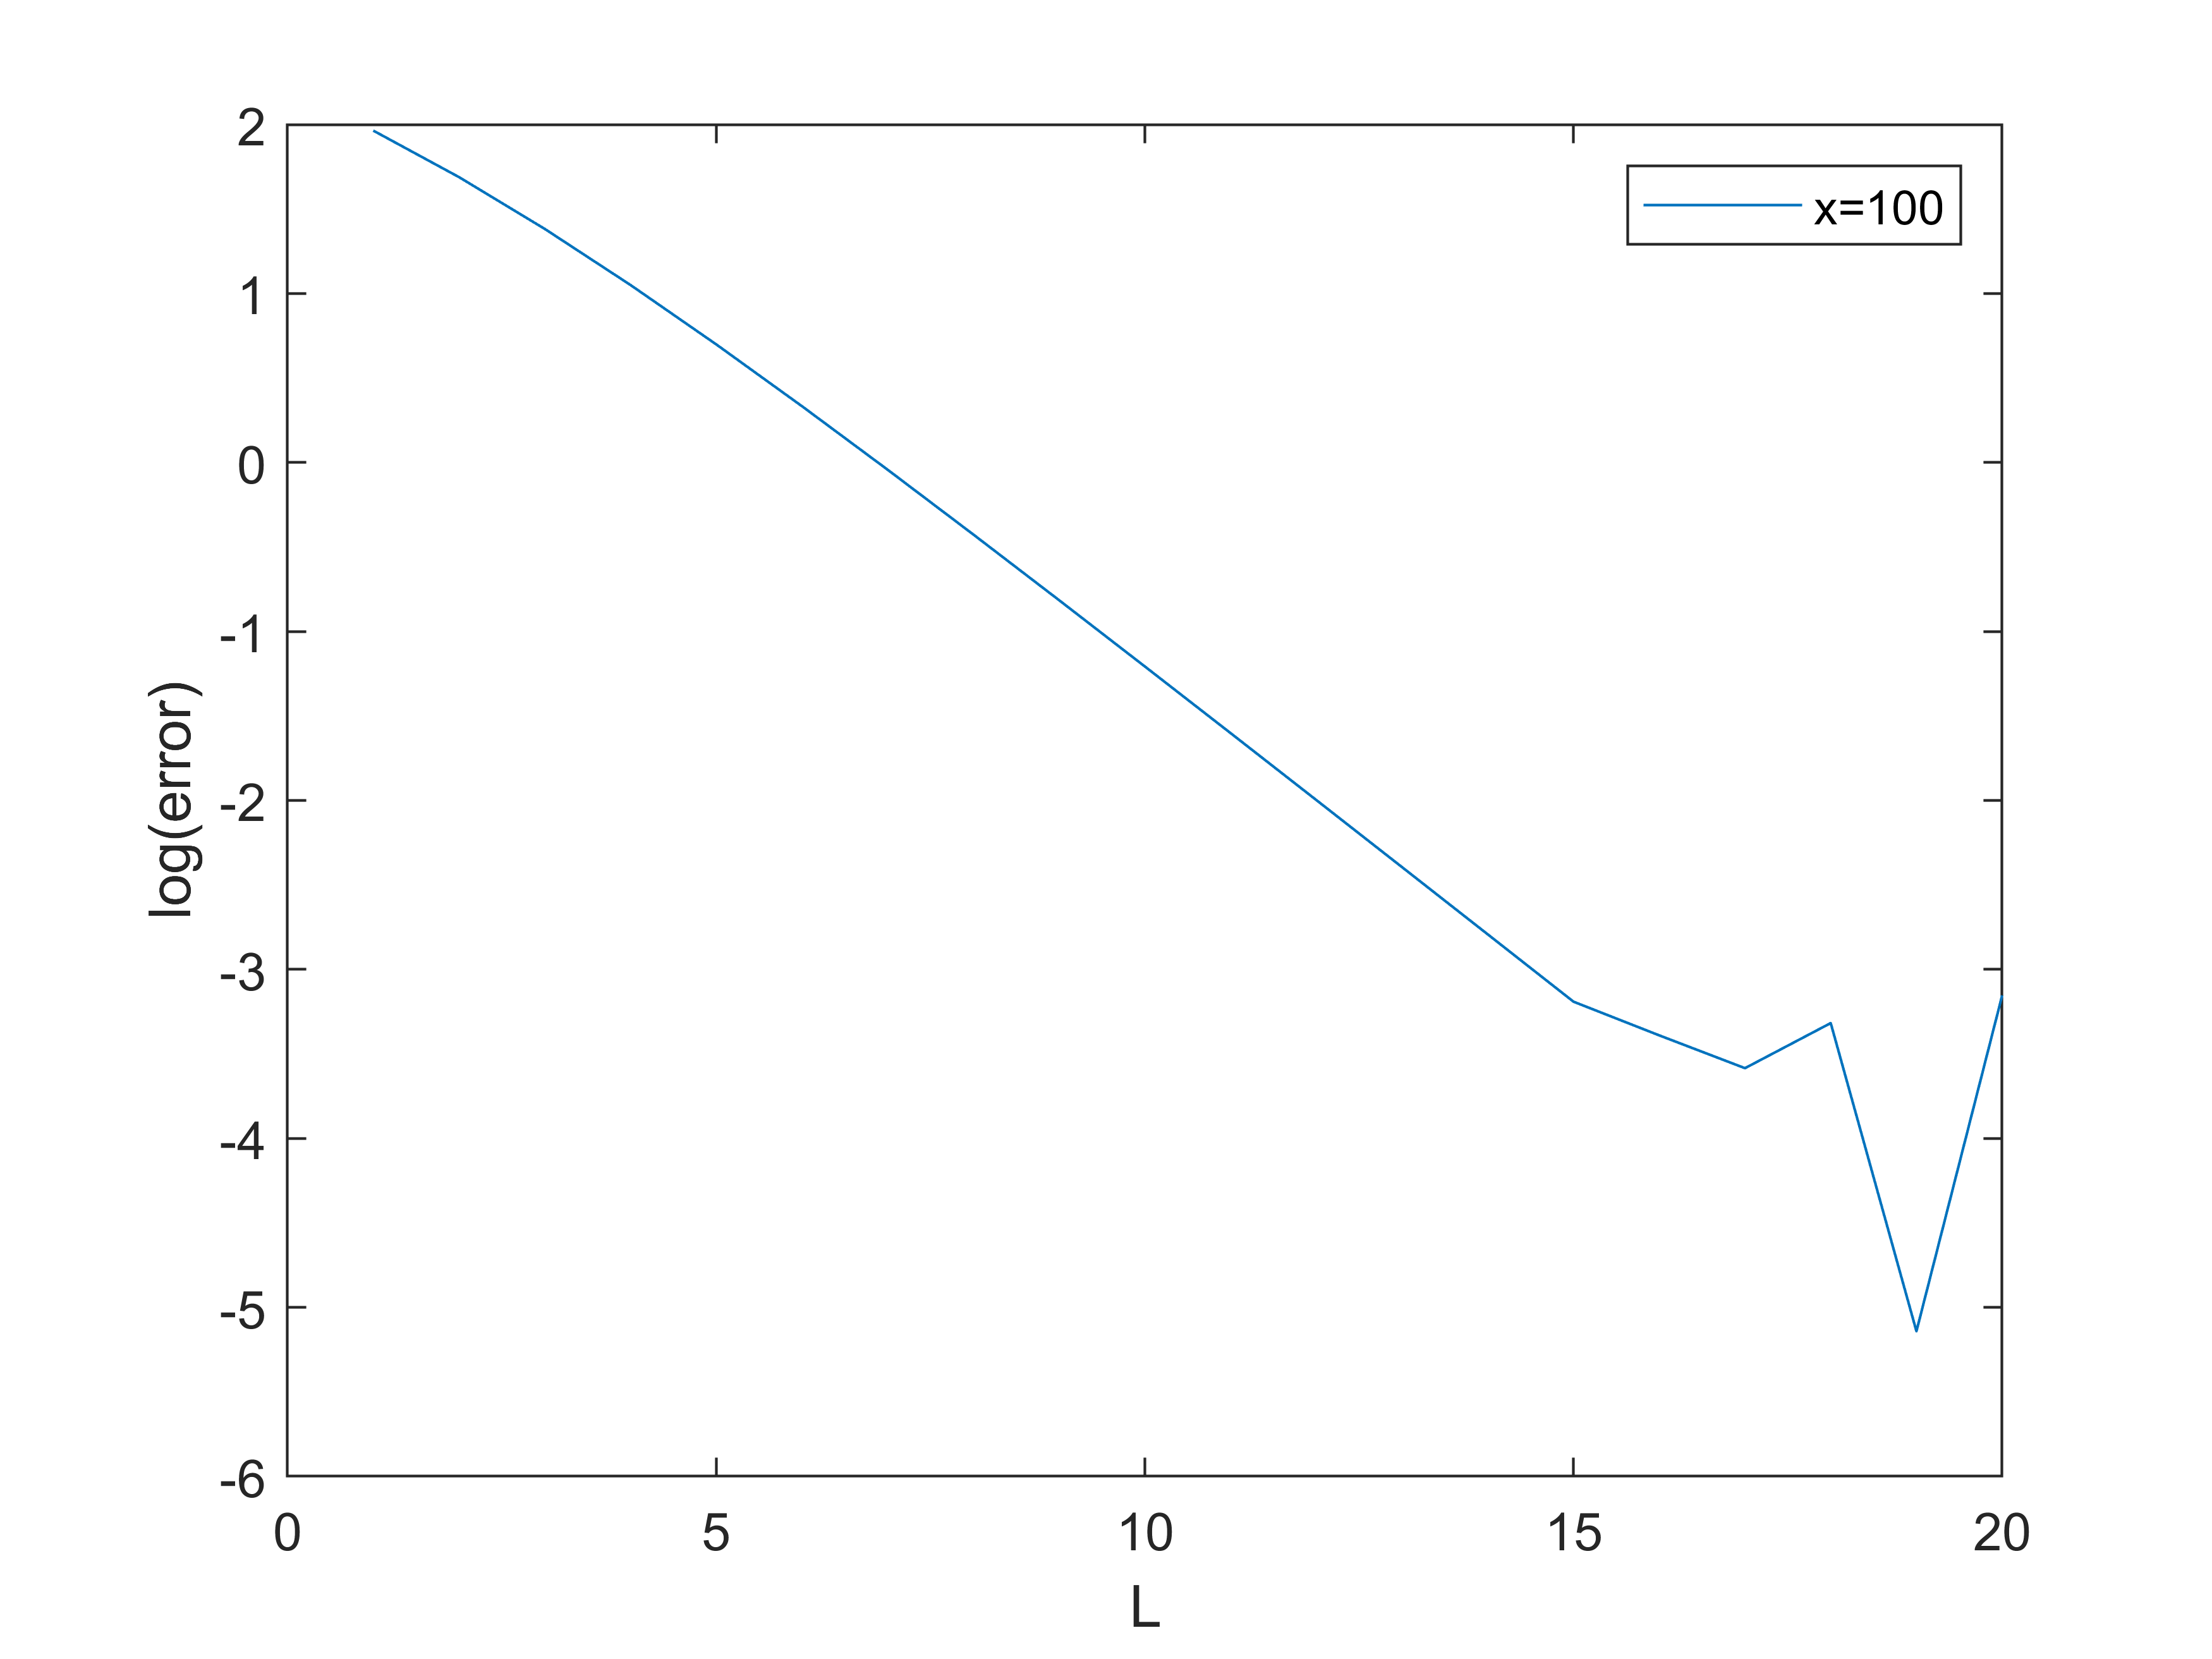
\includegraphics[width=\textwidth]{Files/q3_pp_100_log.png}
            \caption{Graph of Pade approximant error against $L$ at $x=100$}
        \end{minipage}
\end{figure}
\noindent We note that $log(error)$ against $L$ is a straight line in the plots for $L\leq15$ for both $x=10$ and $x=100$.\\
This is the case at $x=10$ because the error is as small as $10^{-16}$ at $L=15$, i.e. the minimum precision of the computer, so it can't get any smaller and the line flattens out.\\
Hence, we try to find the gradient, because if error=$a10^{-k(x)L}$, then $\log$(error)=$c-k(x)L$.\\
And we get $k(10)=1.23990433$ and $k(100)=0.3743033$. We can now guess that $k(x)$ is of the form $cx^a$ where both $c$ and $a$ are constants.\\
Plugging the numbers in, we get $10^a=0.3018808417$, i.e. \underline{$a=-0.52016\approx-\frac{1}{2}$}.\\
Plugging this value of $a$ back in, we get $c=3.92092$ at $x=10$ and $c=3.743033$ at $x=100$. Therefore, the error at $x,L$ is roughly \underline{$\mathcal{O}(10^{-\frac{cL}{\sqrt{x}}})$}.\\
We are able to use the Pade approximant to estimate $f_1(x)$ for large $x$, this implies that the Pade approximant has the same asymptotic behaviour as $f_1(x)$ and they will approach the same asymptotic at a very similar rate.


\subsection*{Question 4}
We now look at the function $f_2(x)=\int^{\infty}_0 e^{-t}(1+xt)^{-1}dt$, and we regard the asymptotic series $1-1!x+2!x^2-3!x^3+4!x^4-5!x^5+\dots$ as its power series. Hence, we note that $c_k=(-1)^kk!$ for the power series. We will compare the truncated power series and the Pade approximants as basis for calculating $f_2(x)$ on the range $0\leq x\leq20$. We will do this by plotting the estimates against $x$ at different values of $N,L$ and compare them to the numerically integrated data.\\
To plot the Pade approximants, we use the program \emph{'ix) q4\textunderscore pade.m'}. In the program, we used a function called \emph{'CoefSolverPS(c,L,M,y)'}, this can be found in the programs section under the title \emph{'x) CoefSolverPS.m'}. This is again very similar to \emph{'CoefSolver.m'}, the only difference is that \emph{'CoefSolverPS.m'} takes the coefficients of the power series as input rather than the raw function $f_2$.\\
We will first plot the Pade appproximant estimation when $L=3,7,11,15$.
\begin{figure}[H]
\centering
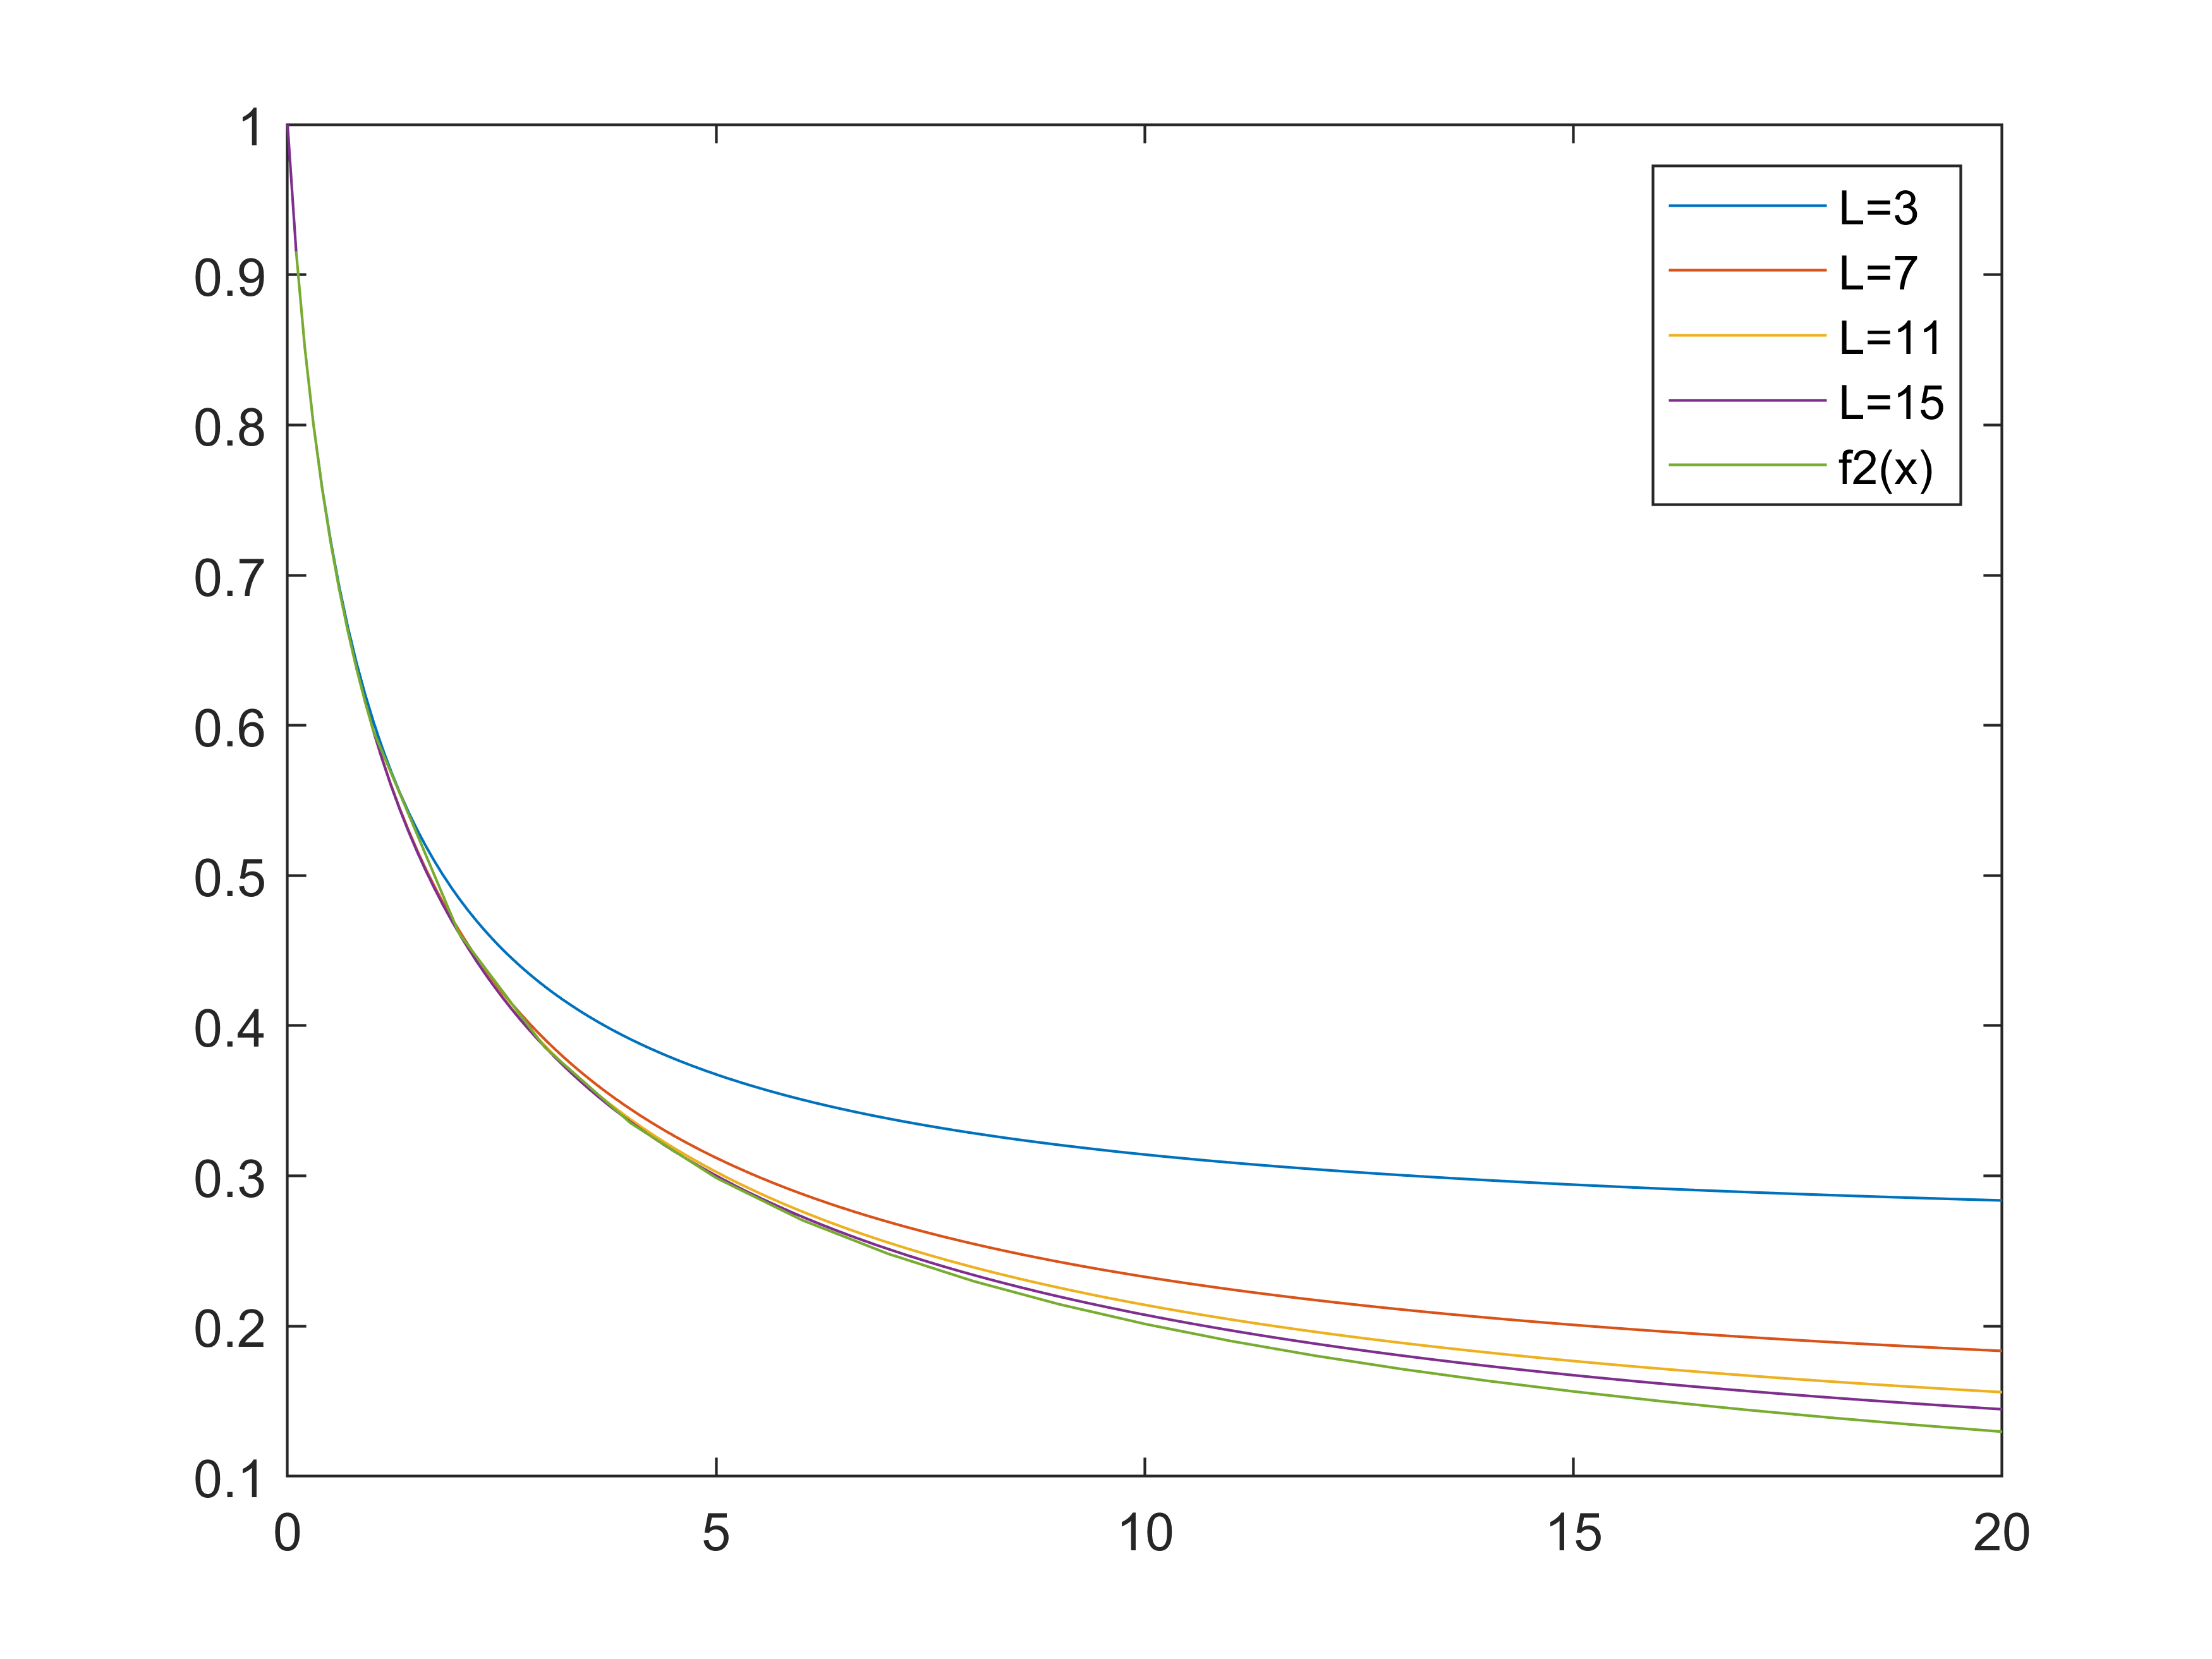
\includegraphics[width=0.5\textwidth]{Files/q4,L=3,7,11,15.png}
\caption{Graph of $R_{L,L}(x)$ against $x$ for $L=3,7,11,15$ and $x\in[0,20]$}
\end{figure}
\noindent We note that as $L$ increases, the error between $f_2(x)$ and the estimate $R_{L,L}(x)$ decreases. In fact, when $L=15$, we've got a very reasonable estimate of $f_2(x)$ especially at large values of $x$. The error is also larger when $x$ is larger.\\
We can therefore conclude that the Pade approximants would be a good basis for calculating $f_2(x)$ on the range $0\leq x\leq20$, as it is converging to $f_2(x)$ as $L\to\infty$, and the rate isn't very slow.\\
However, for the truncated power series, this isn't necessarily the case. The program we use to plot the power series is \emph{'xi) q4\textunderscore power\textunderscore series.m'}.\\
\begin{figure}[H]
\centering
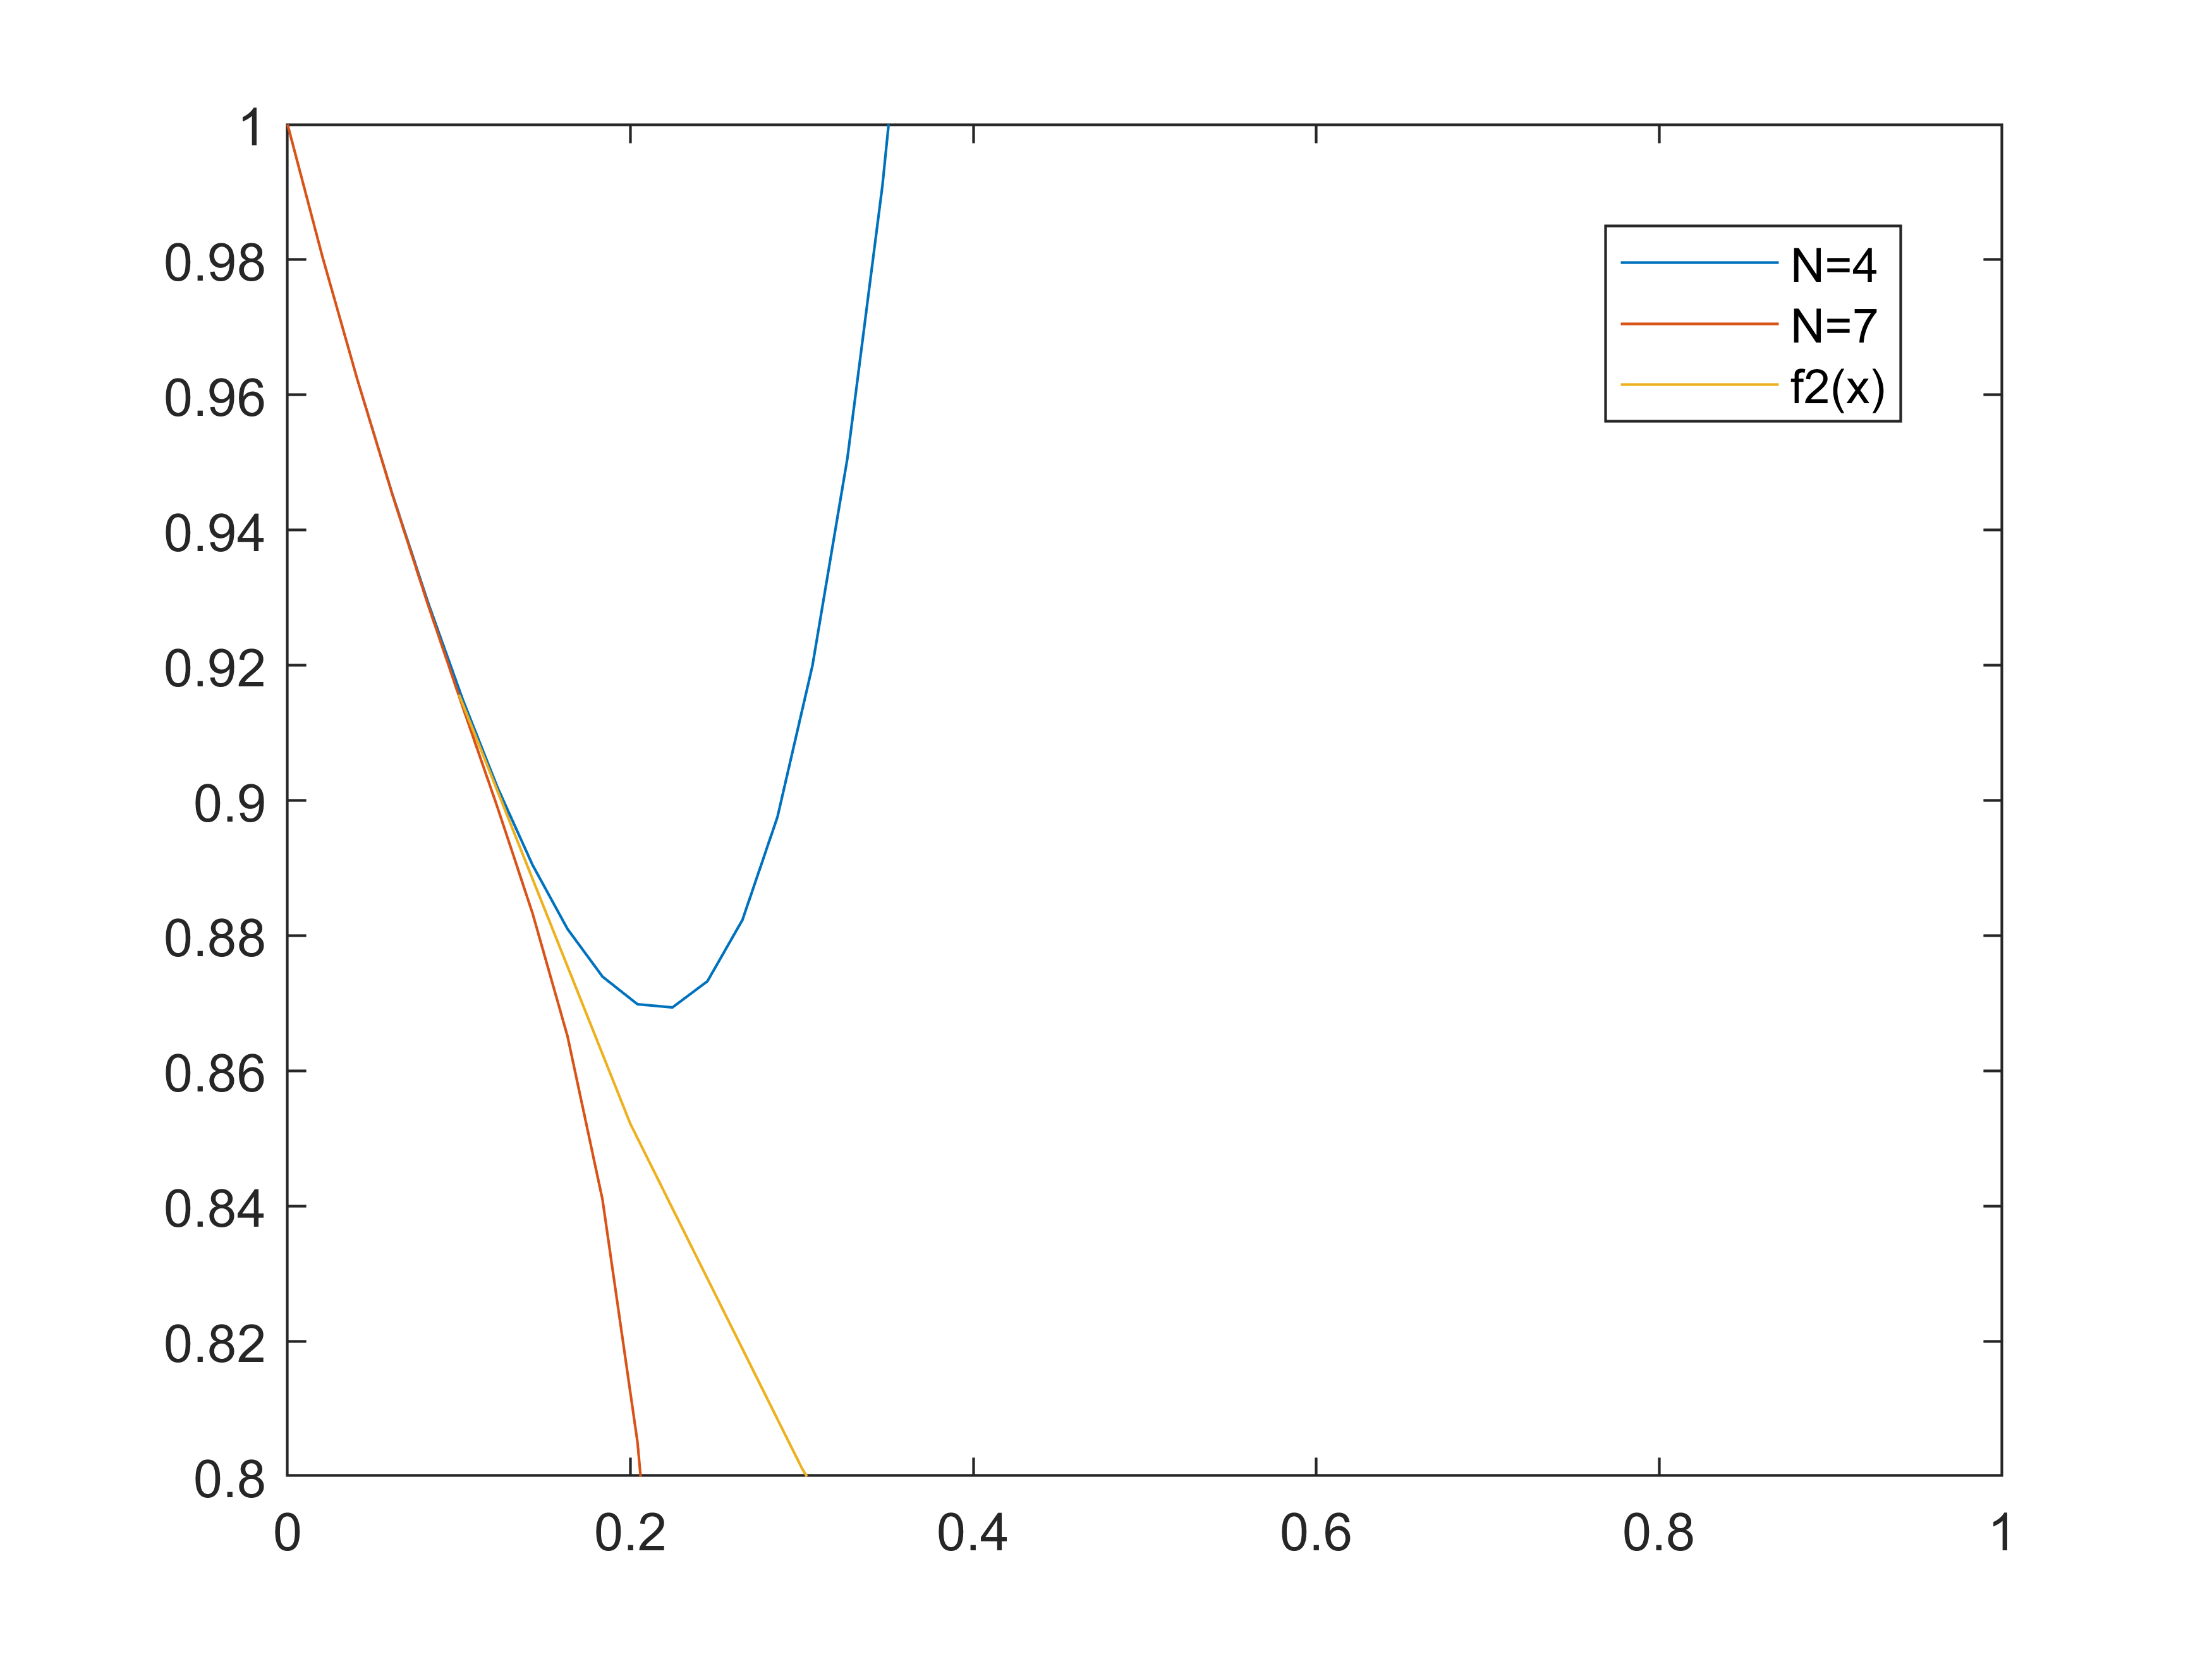
\includegraphics[width=0.5\textwidth]{Files/q4,N=4,7.png}
\caption{Graph of truncated power series against $x$ for $N=4,7$ and $x\in[0,1]$}
\end{figure}
\noindent We know that the truncated series is only a "good" approximation of $f_2(x)$ when $x$ is "small", and we can see that this is indeed the case in the graph.\\
When $x\in[0.1,0.16]$, the truncated power series can approximate $f_2(x)$ quite well, with relatively small error. However, as $x$ grows, the power series diverge from $f_2(x)$, and the rate of divergence is actually greater for larger $N$. Hence, the truncated power series is not a good basis for calculating $f_2(x)$ on the range $0\leq x\leq 20$. However, it'd be an alright approximation for a much smaller range of $x$, where $x<<1$.


\section*{3 Zeroes and poles}
\medskip
\subsection*{Question 5}
The functions we want to investigate are $f_1(x)=(1+x)^{1/2}, f_3(x)=(1+x)^{-1/2},f_4(x)=e^x,f_5(x)=e^x/(1+x)$ and $f_6(x)=(1+x+x^2)^{1/2}$.\\
The program we use to do so is \emph{'xii) q5.m'}. To find the zeros, we calculate the roots of the numerator polynomial and to find the poles, we calculate the roots of the denominator polynomial.\\
\textbf{With $f_1$}, we first look at what happens when $L=[7,11]$
\begin{figure}[H]
    \begin{minipage}[b]{0.47\linewidth}
            \centering
            \textbf{L=7}\par
            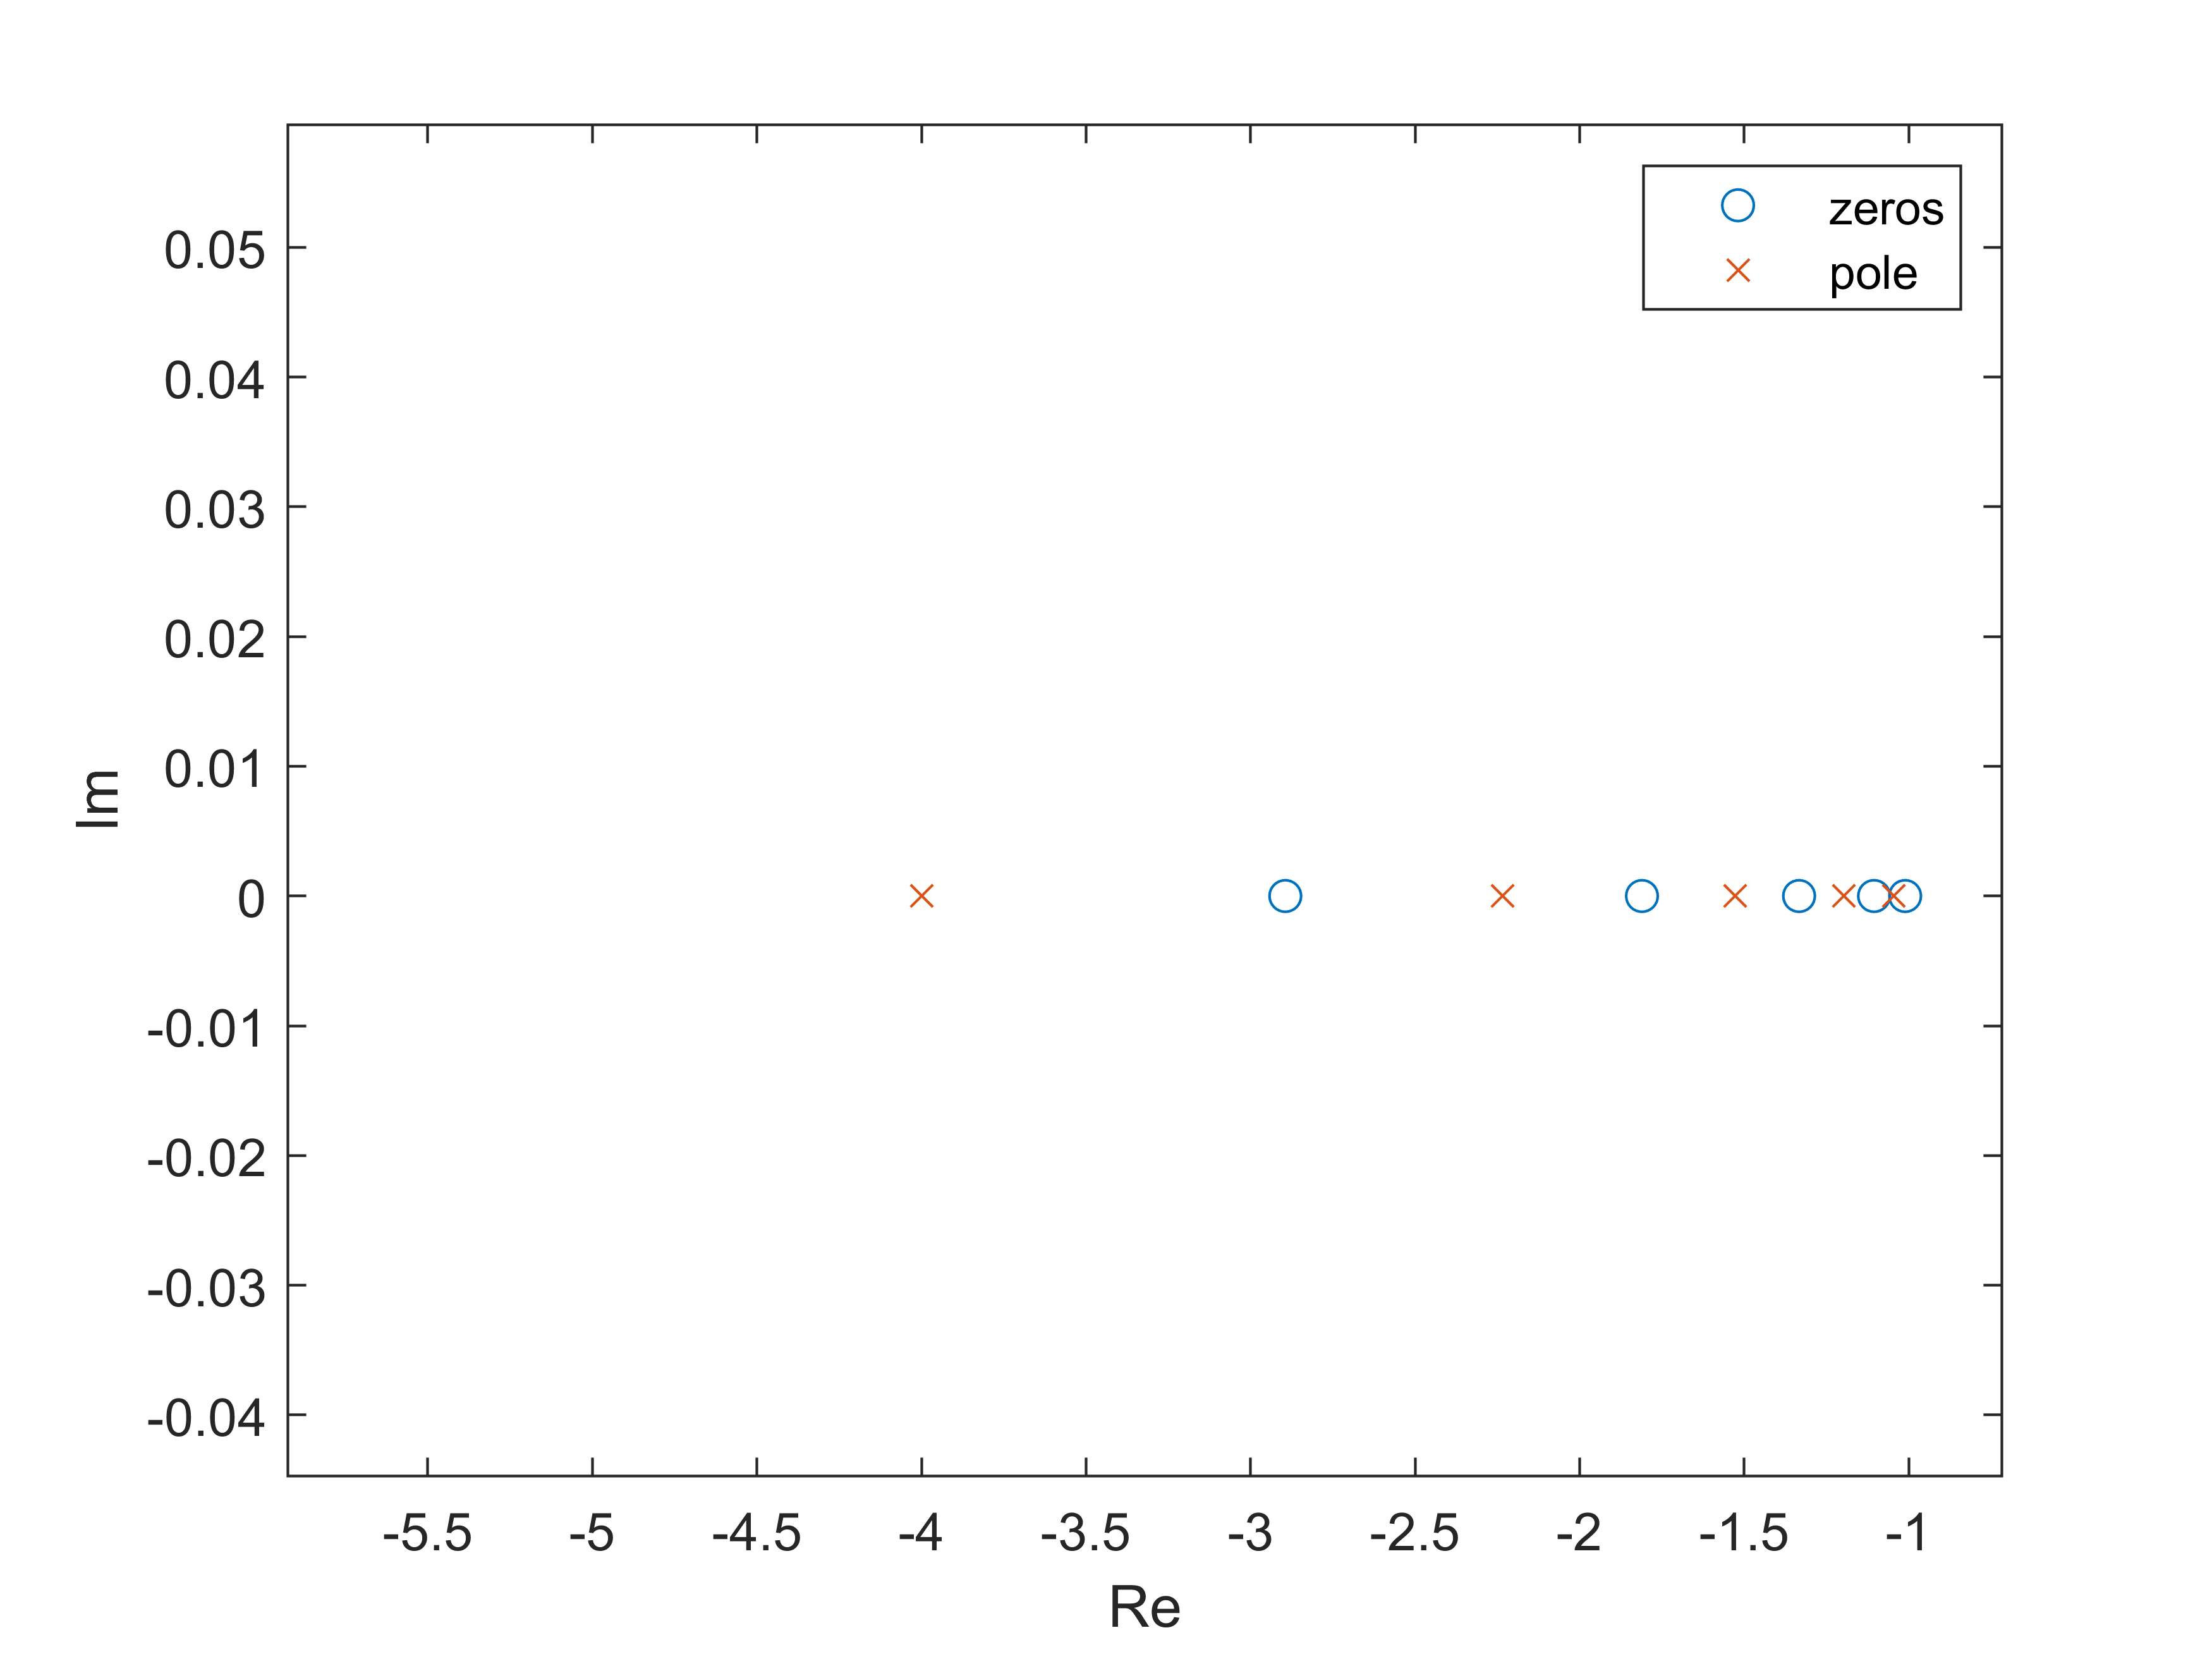
\includegraphics[width=\textwidth]{Files/q5,f1,7.png}
            \caption{Pole-Zero plot of $R_{7,7}(f_1)$}
        \end{minipage}
        \hfill
            \begin{minipage}[b]{0.47\linewidth}
            \centering
    \textbf{L=11}\par
    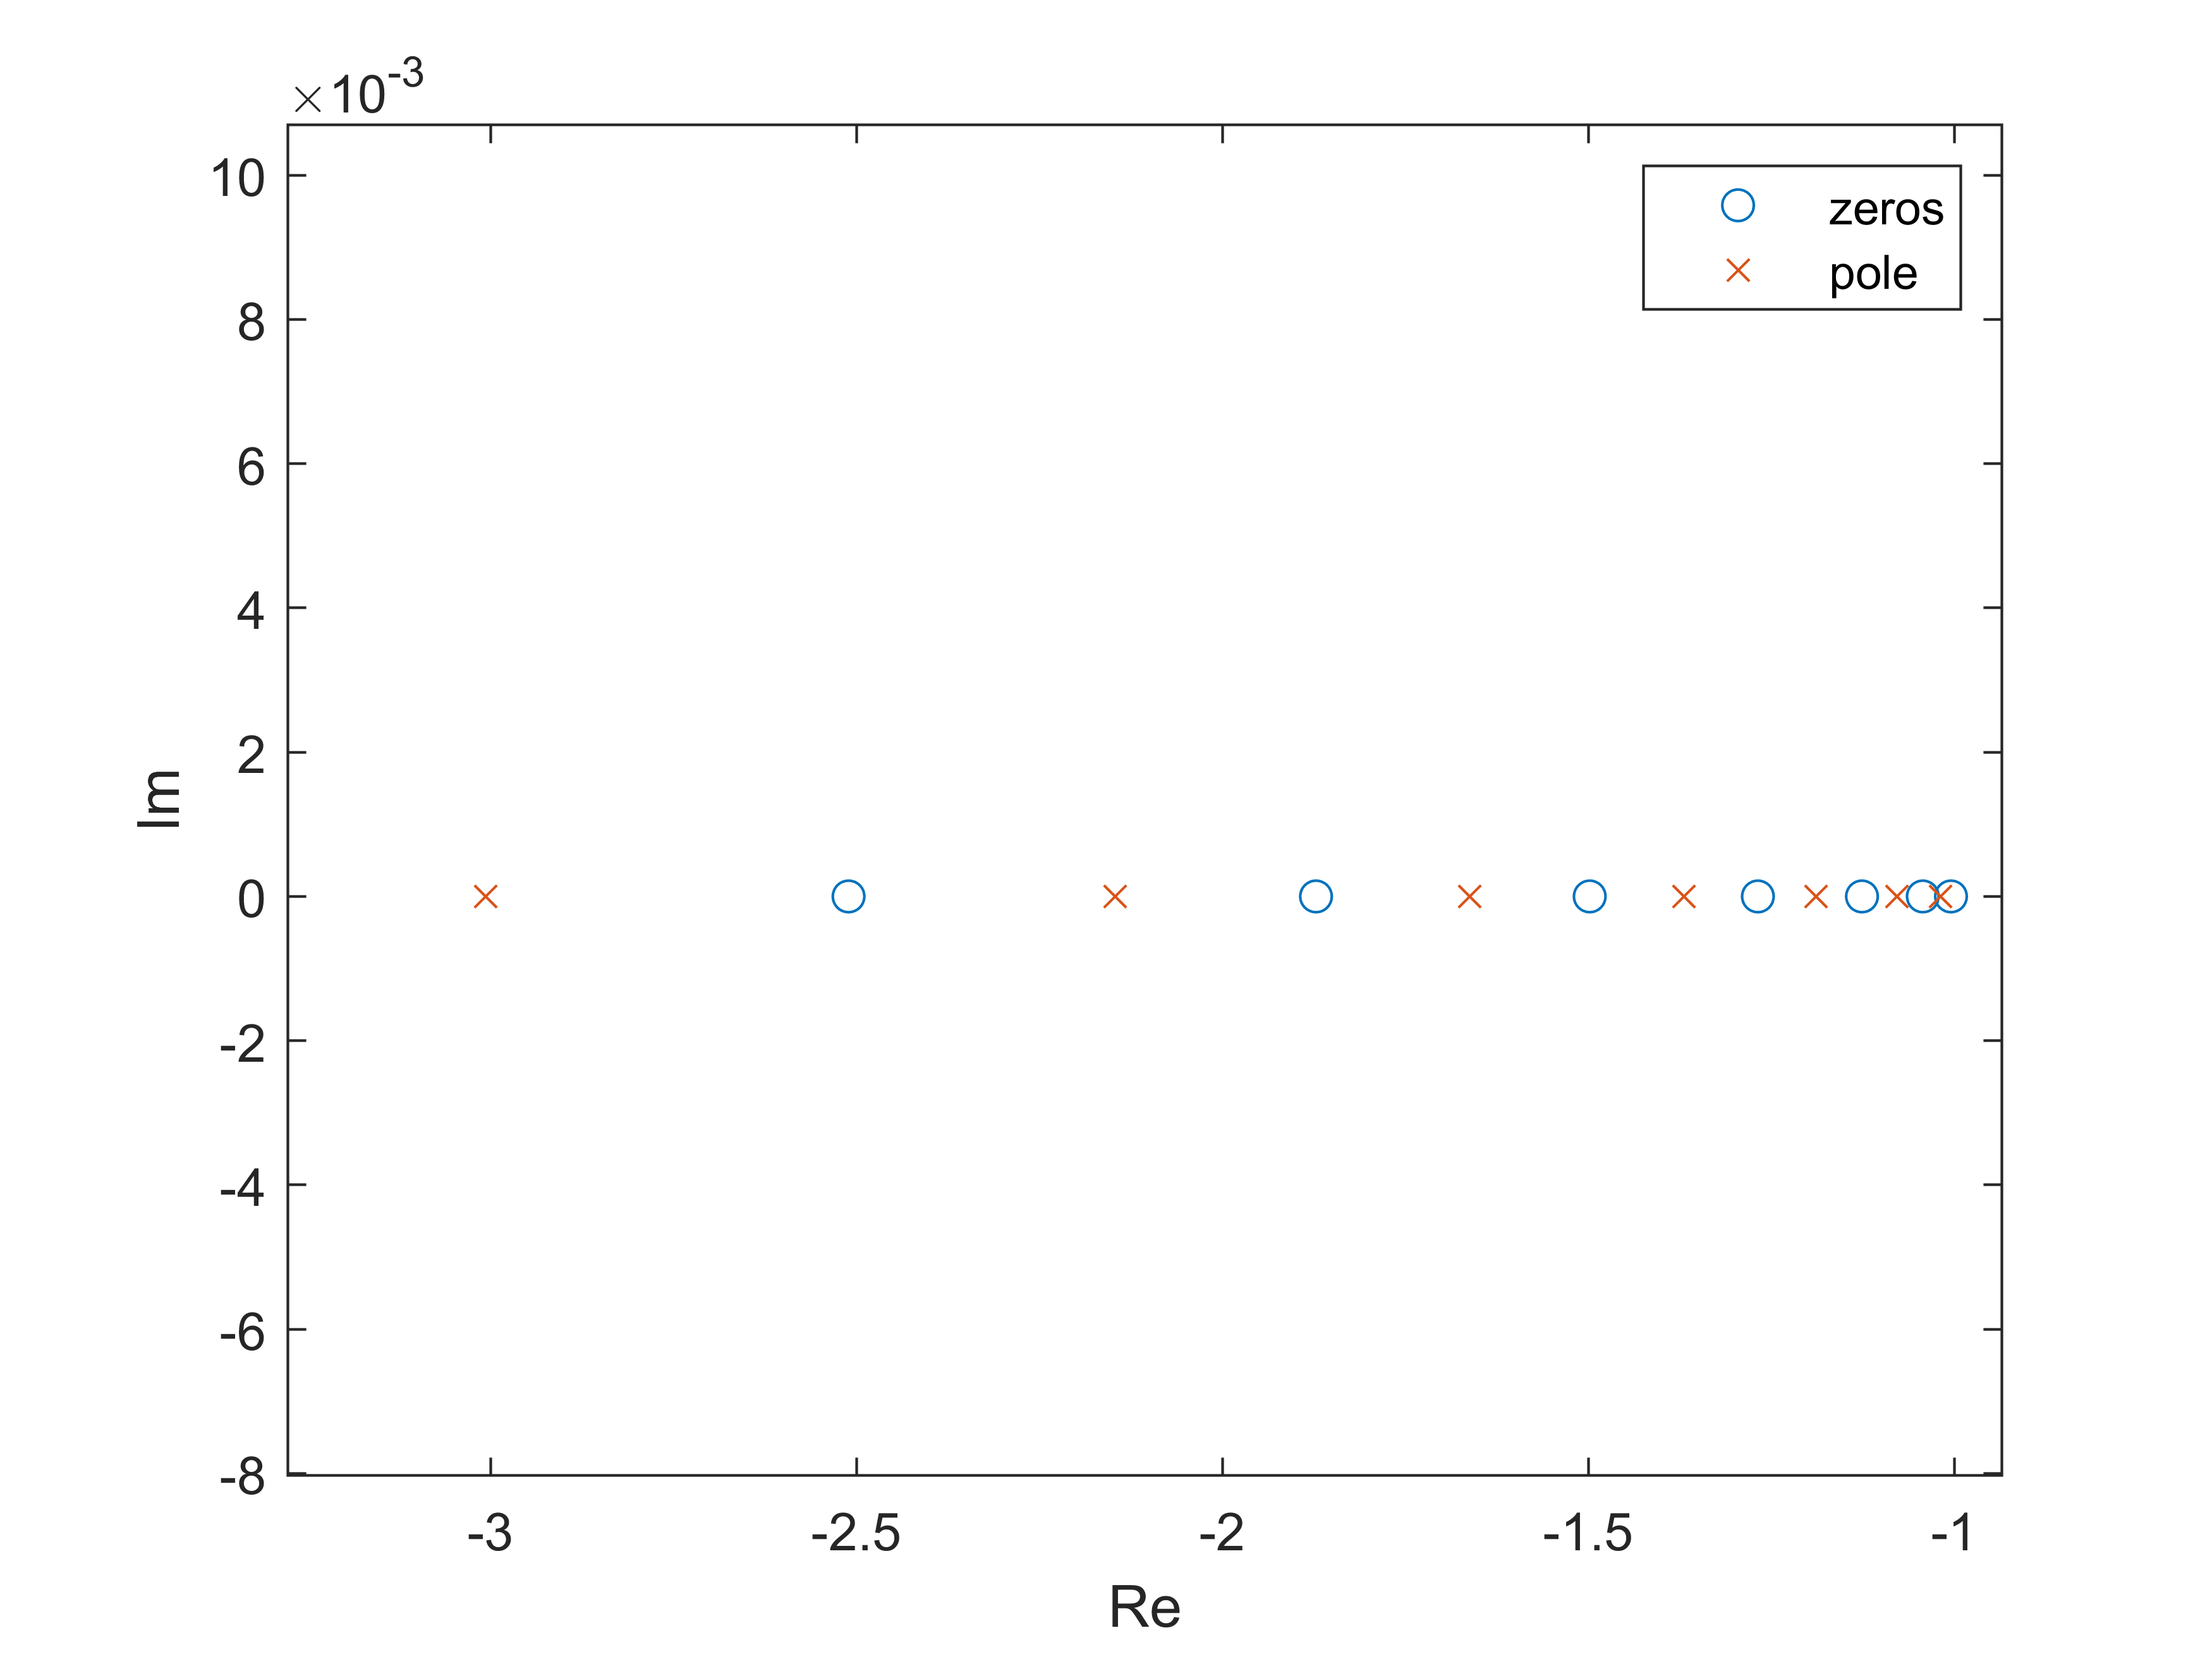
\includegraphics[width=\textwidth]{Files/q5,f1,11.png}
    \caption{Pole-Zero plot of $R_{11,11}(f_1)$}
        \end{minipage}
\end{figure}
\noindent We first notice that all the zeros and poles of $R_{L,L}(x)$ for $f_1(x)$ are real and negative. Coming from negative infinity on the real axis, we always encounter a pole first, then a zero, and they will repeat this alternating pattern until we encounter the final zero which is always left to $(-1,0)$. The distance between each pole and zero is always decreasing if we start counting from the most negative zero.\\
As $L$ increases, the position of the poles and zeros all shift in the positive real direction and their distance to $(-1,0)$ shrinks.\\\\
\textbf{With $f_3$}, we will look at $L=[7,11]$ again.\\
\begin{figure}[H]
    \begin{minipage}[b]{0.47\linewidth}
            \centering
            \textbf{L=7}\par
            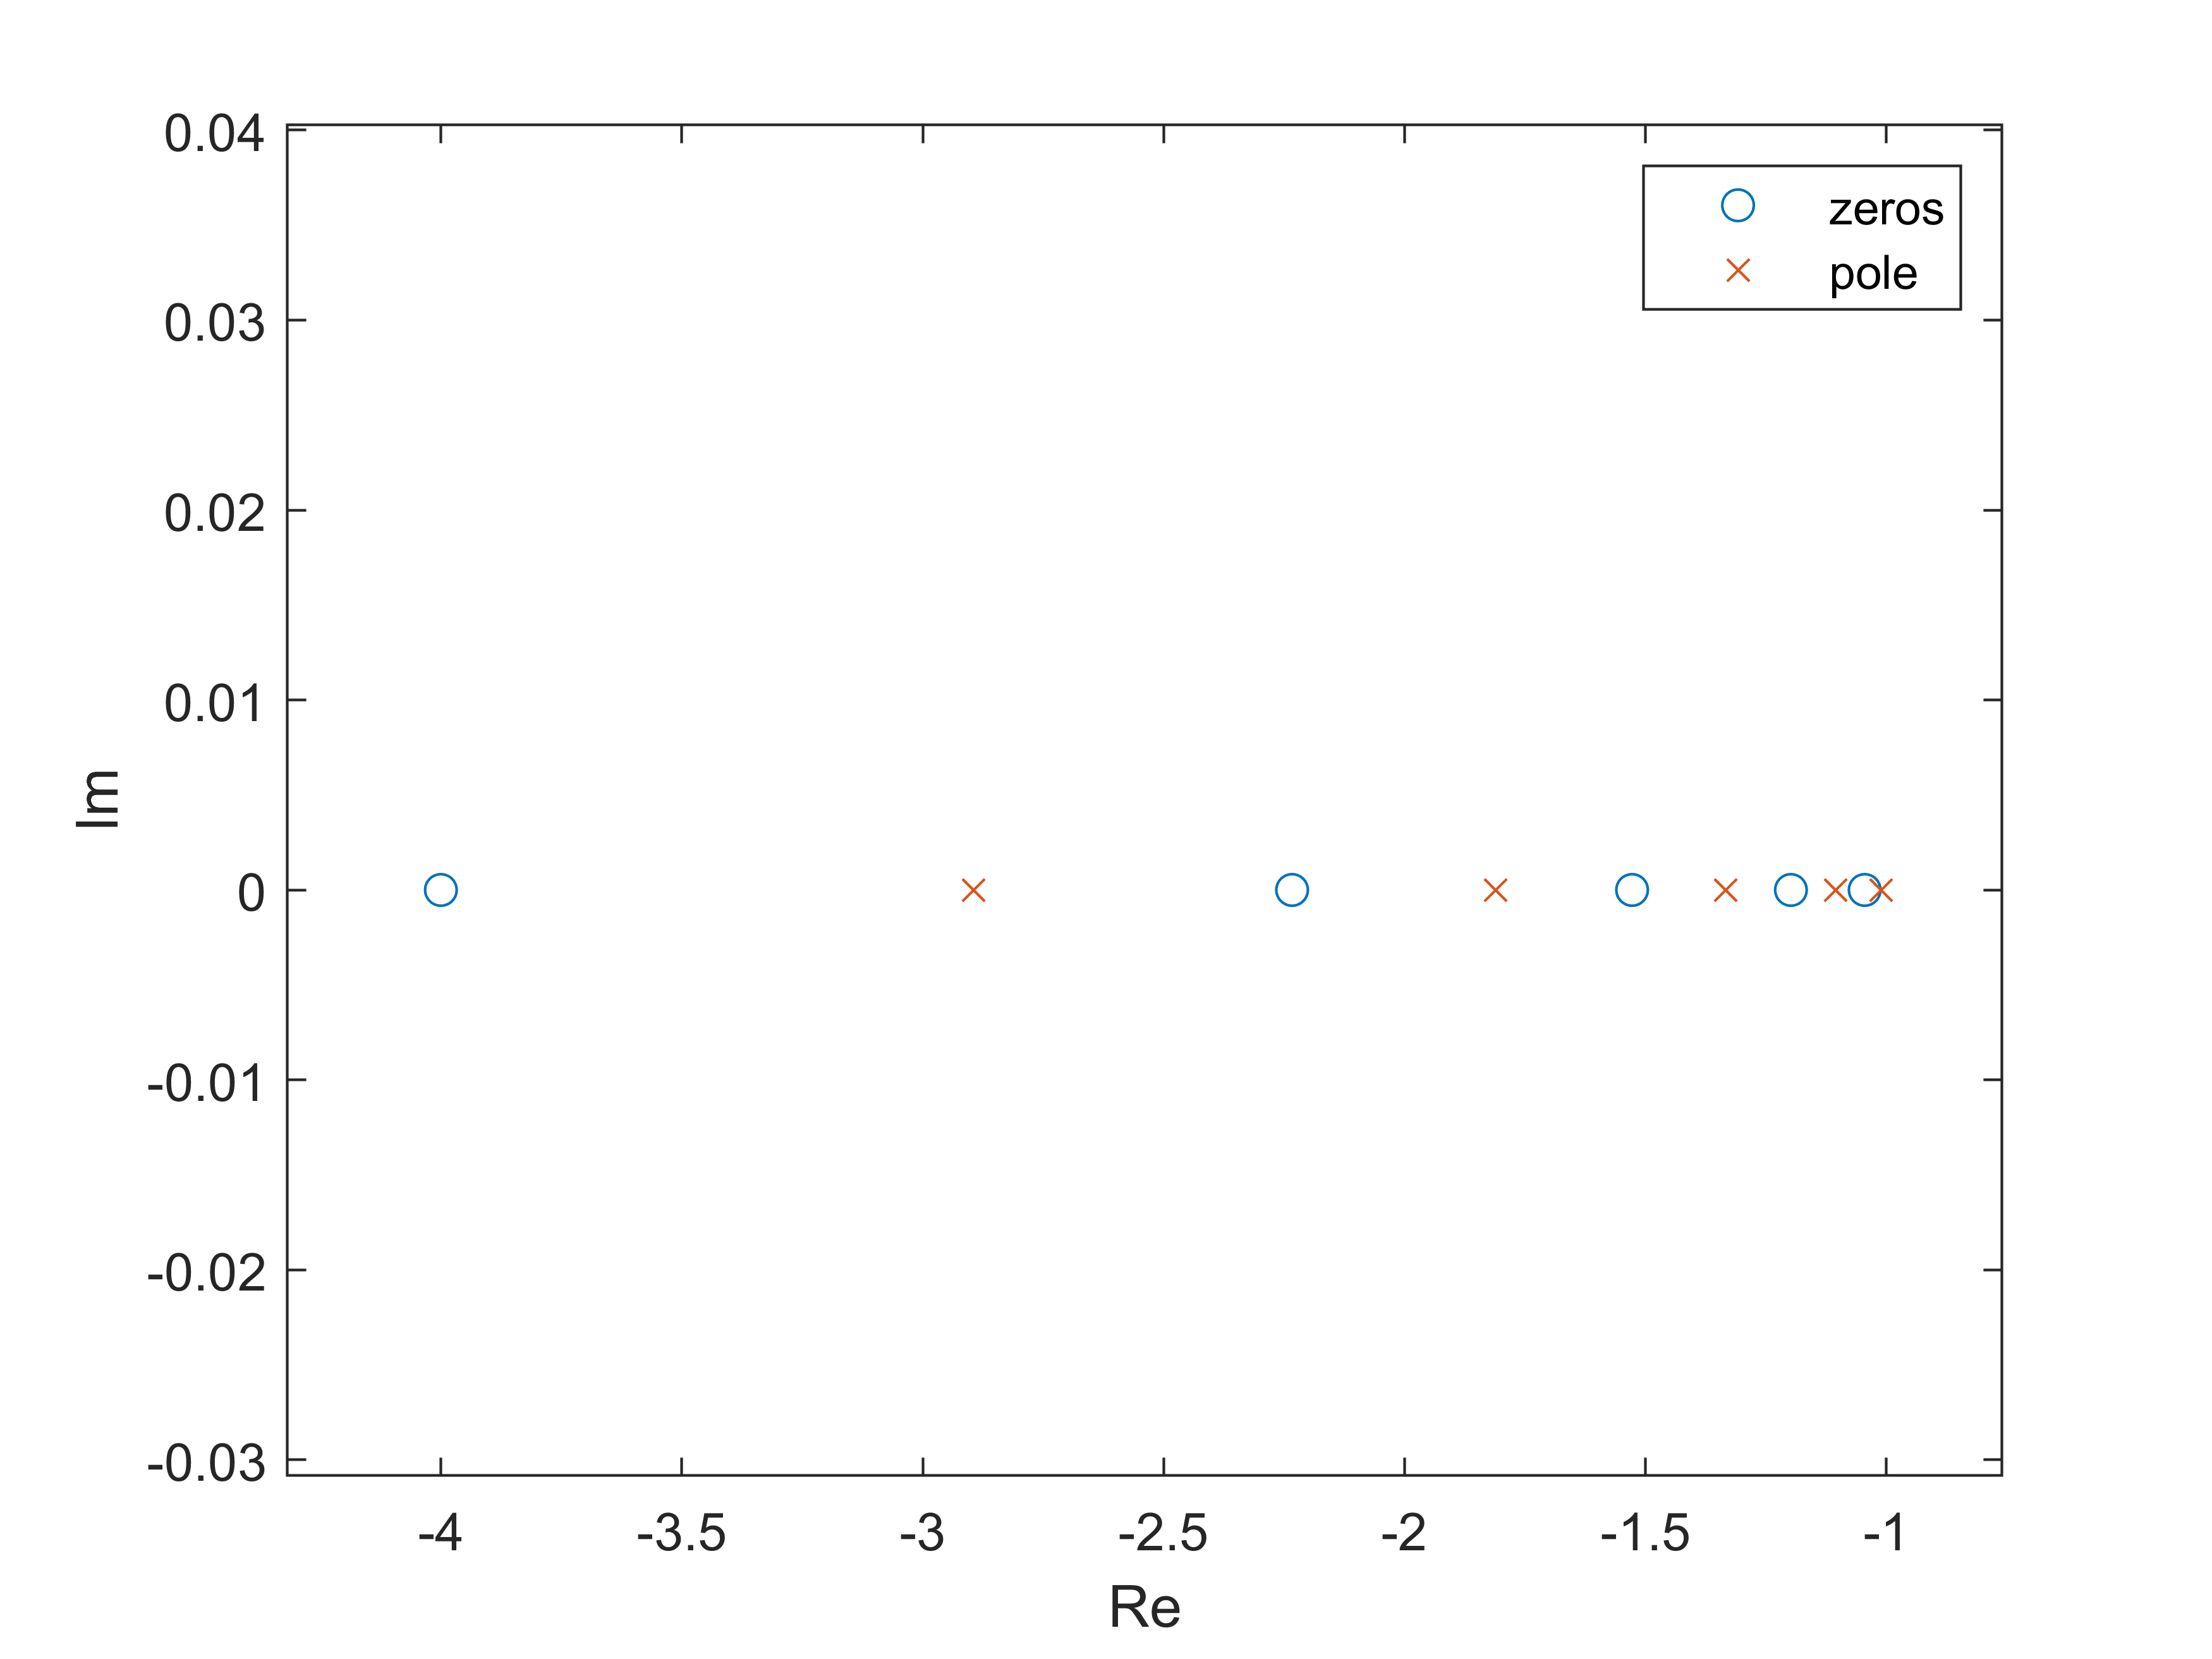
\includegraphics[width=\textwidth]{Files/q5,f3,7.png}
            \caption{Pole-Zero plot of $R_{7,7}(f_3)$}
        \end{minipage}
        \hfill
            \begin{minipage}[b]{0.47\linewidth}
            \centering
    \textbf{L=11}\par
    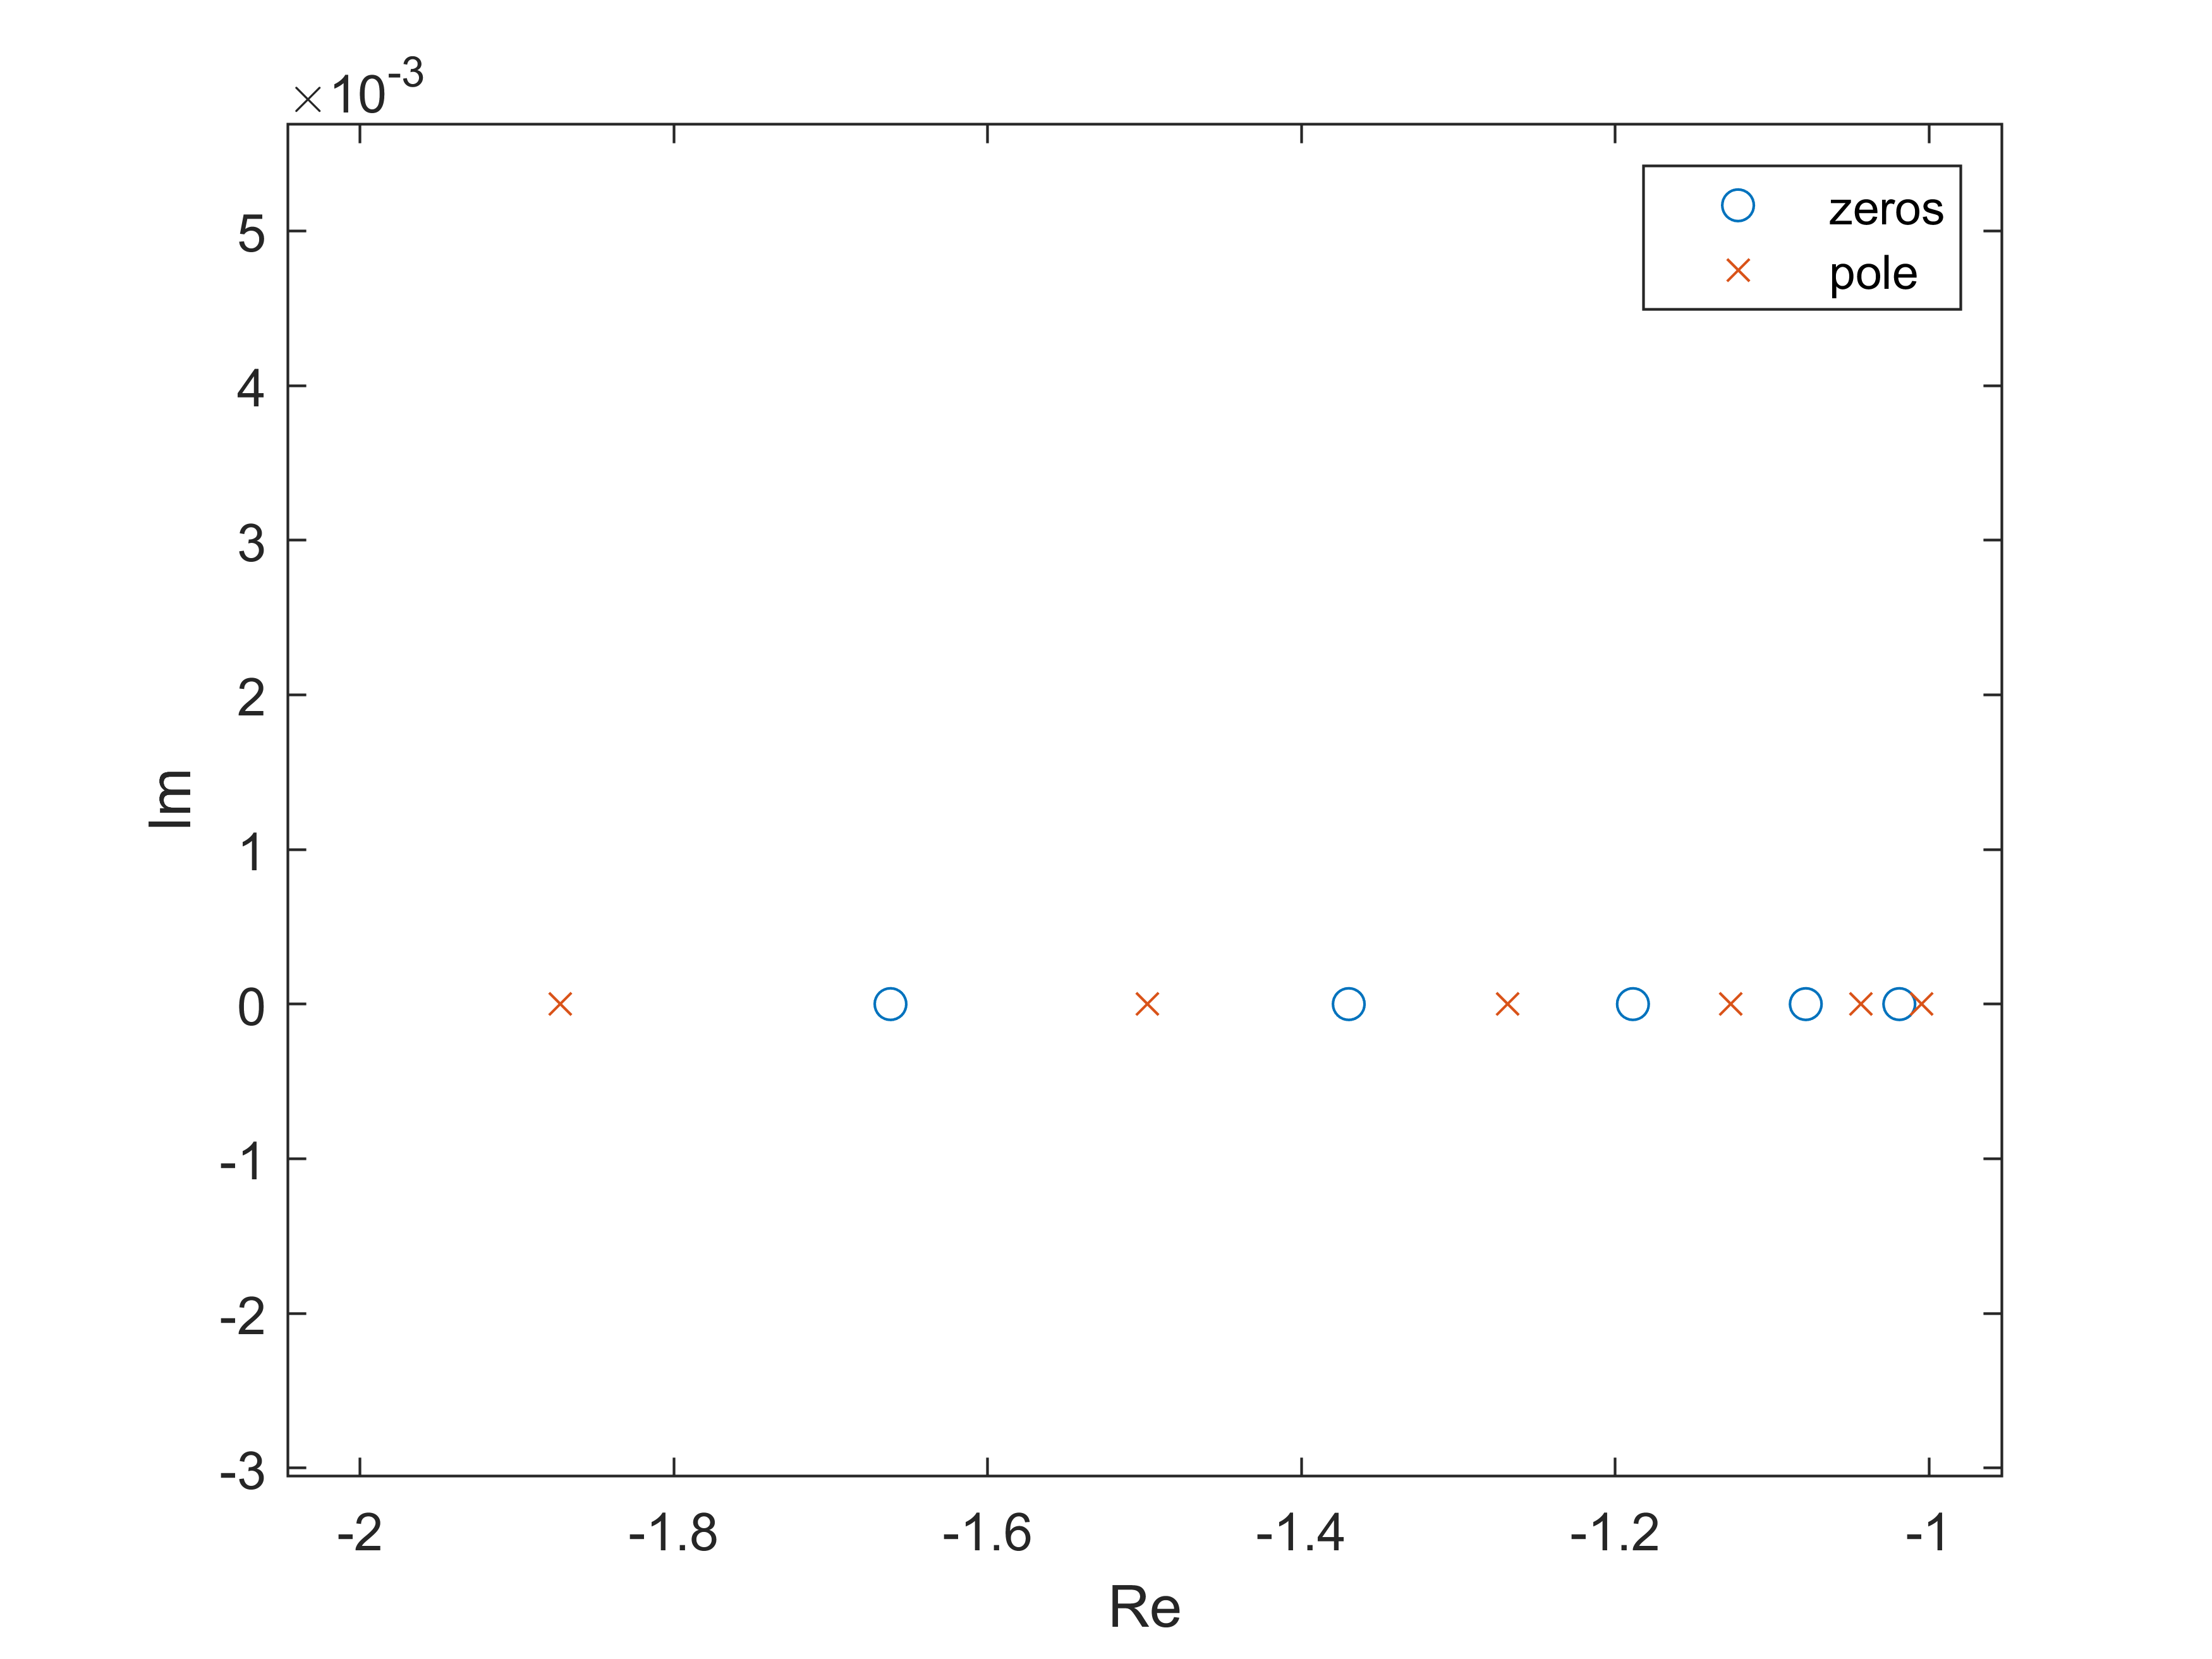
\includegraphics[width=\textwidth]{Files/q5,f3,11.png}
    \caption{Pole-Zero plot of $R_{11,11}(f_3)$}
        \end{minipage}
\end{figure}
\noindent We notice that when we compare the numerical values of the poles and zeros in $R_{L,L}(f_3)$ and $R_{L,L}(f_1)$, the poles in $f_3$ have the exact same position as the zeros in $f_1$, and the zeros in $f_3$ have the exact same position as the poles in $f_1$ for fixed $L$. And they observe the same pattern of positional change as $L$ increases.\\\\
With $f_4$, we will look at $L=7,11$ again.\\
\begin{figure}[H]
    \begin{minipage}[b]{0.47\linewidth}
            \centering
            \textbf{L=7}\par
            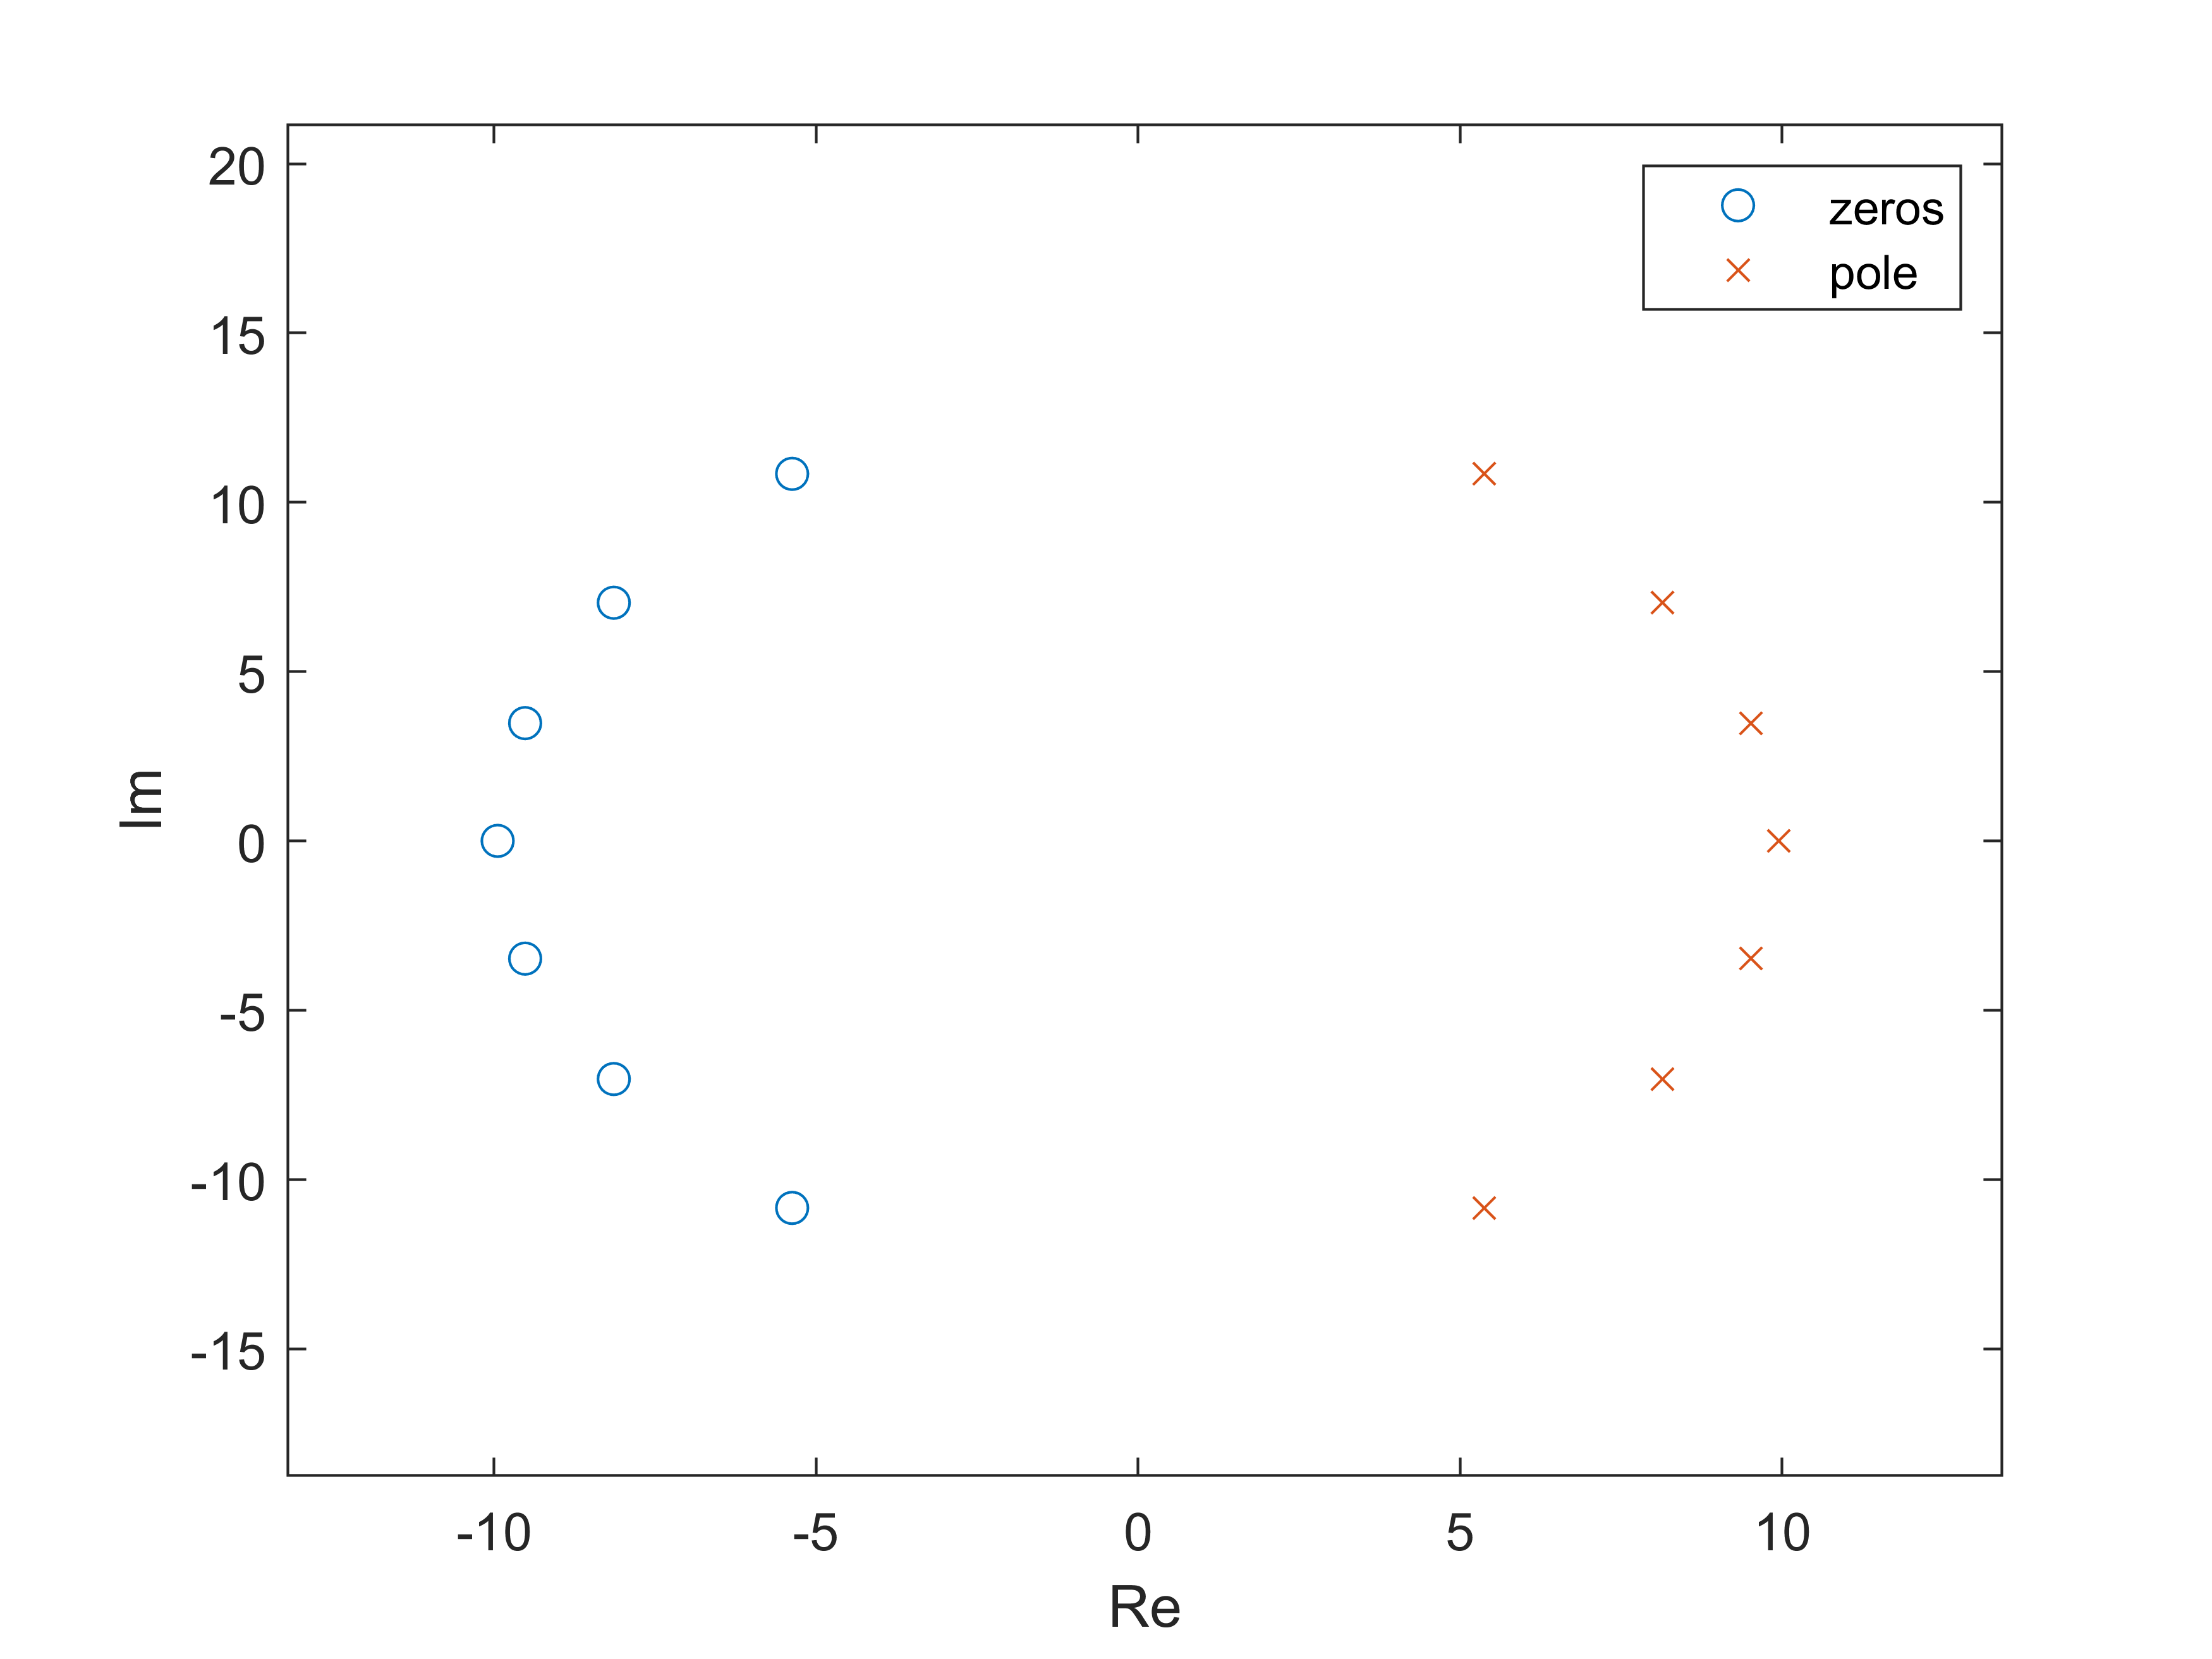
\includegraphics[width=\textwidth]{Files/q5,f4,7.png}
            \caption{Pole-Zero plot of $R_{7,7}(f_4)$}
        \end{minipage}
        \hfill
            \begin{minipage}[b]{0.47\linewidth}
            \centering
    \textbf{L=11}\par
    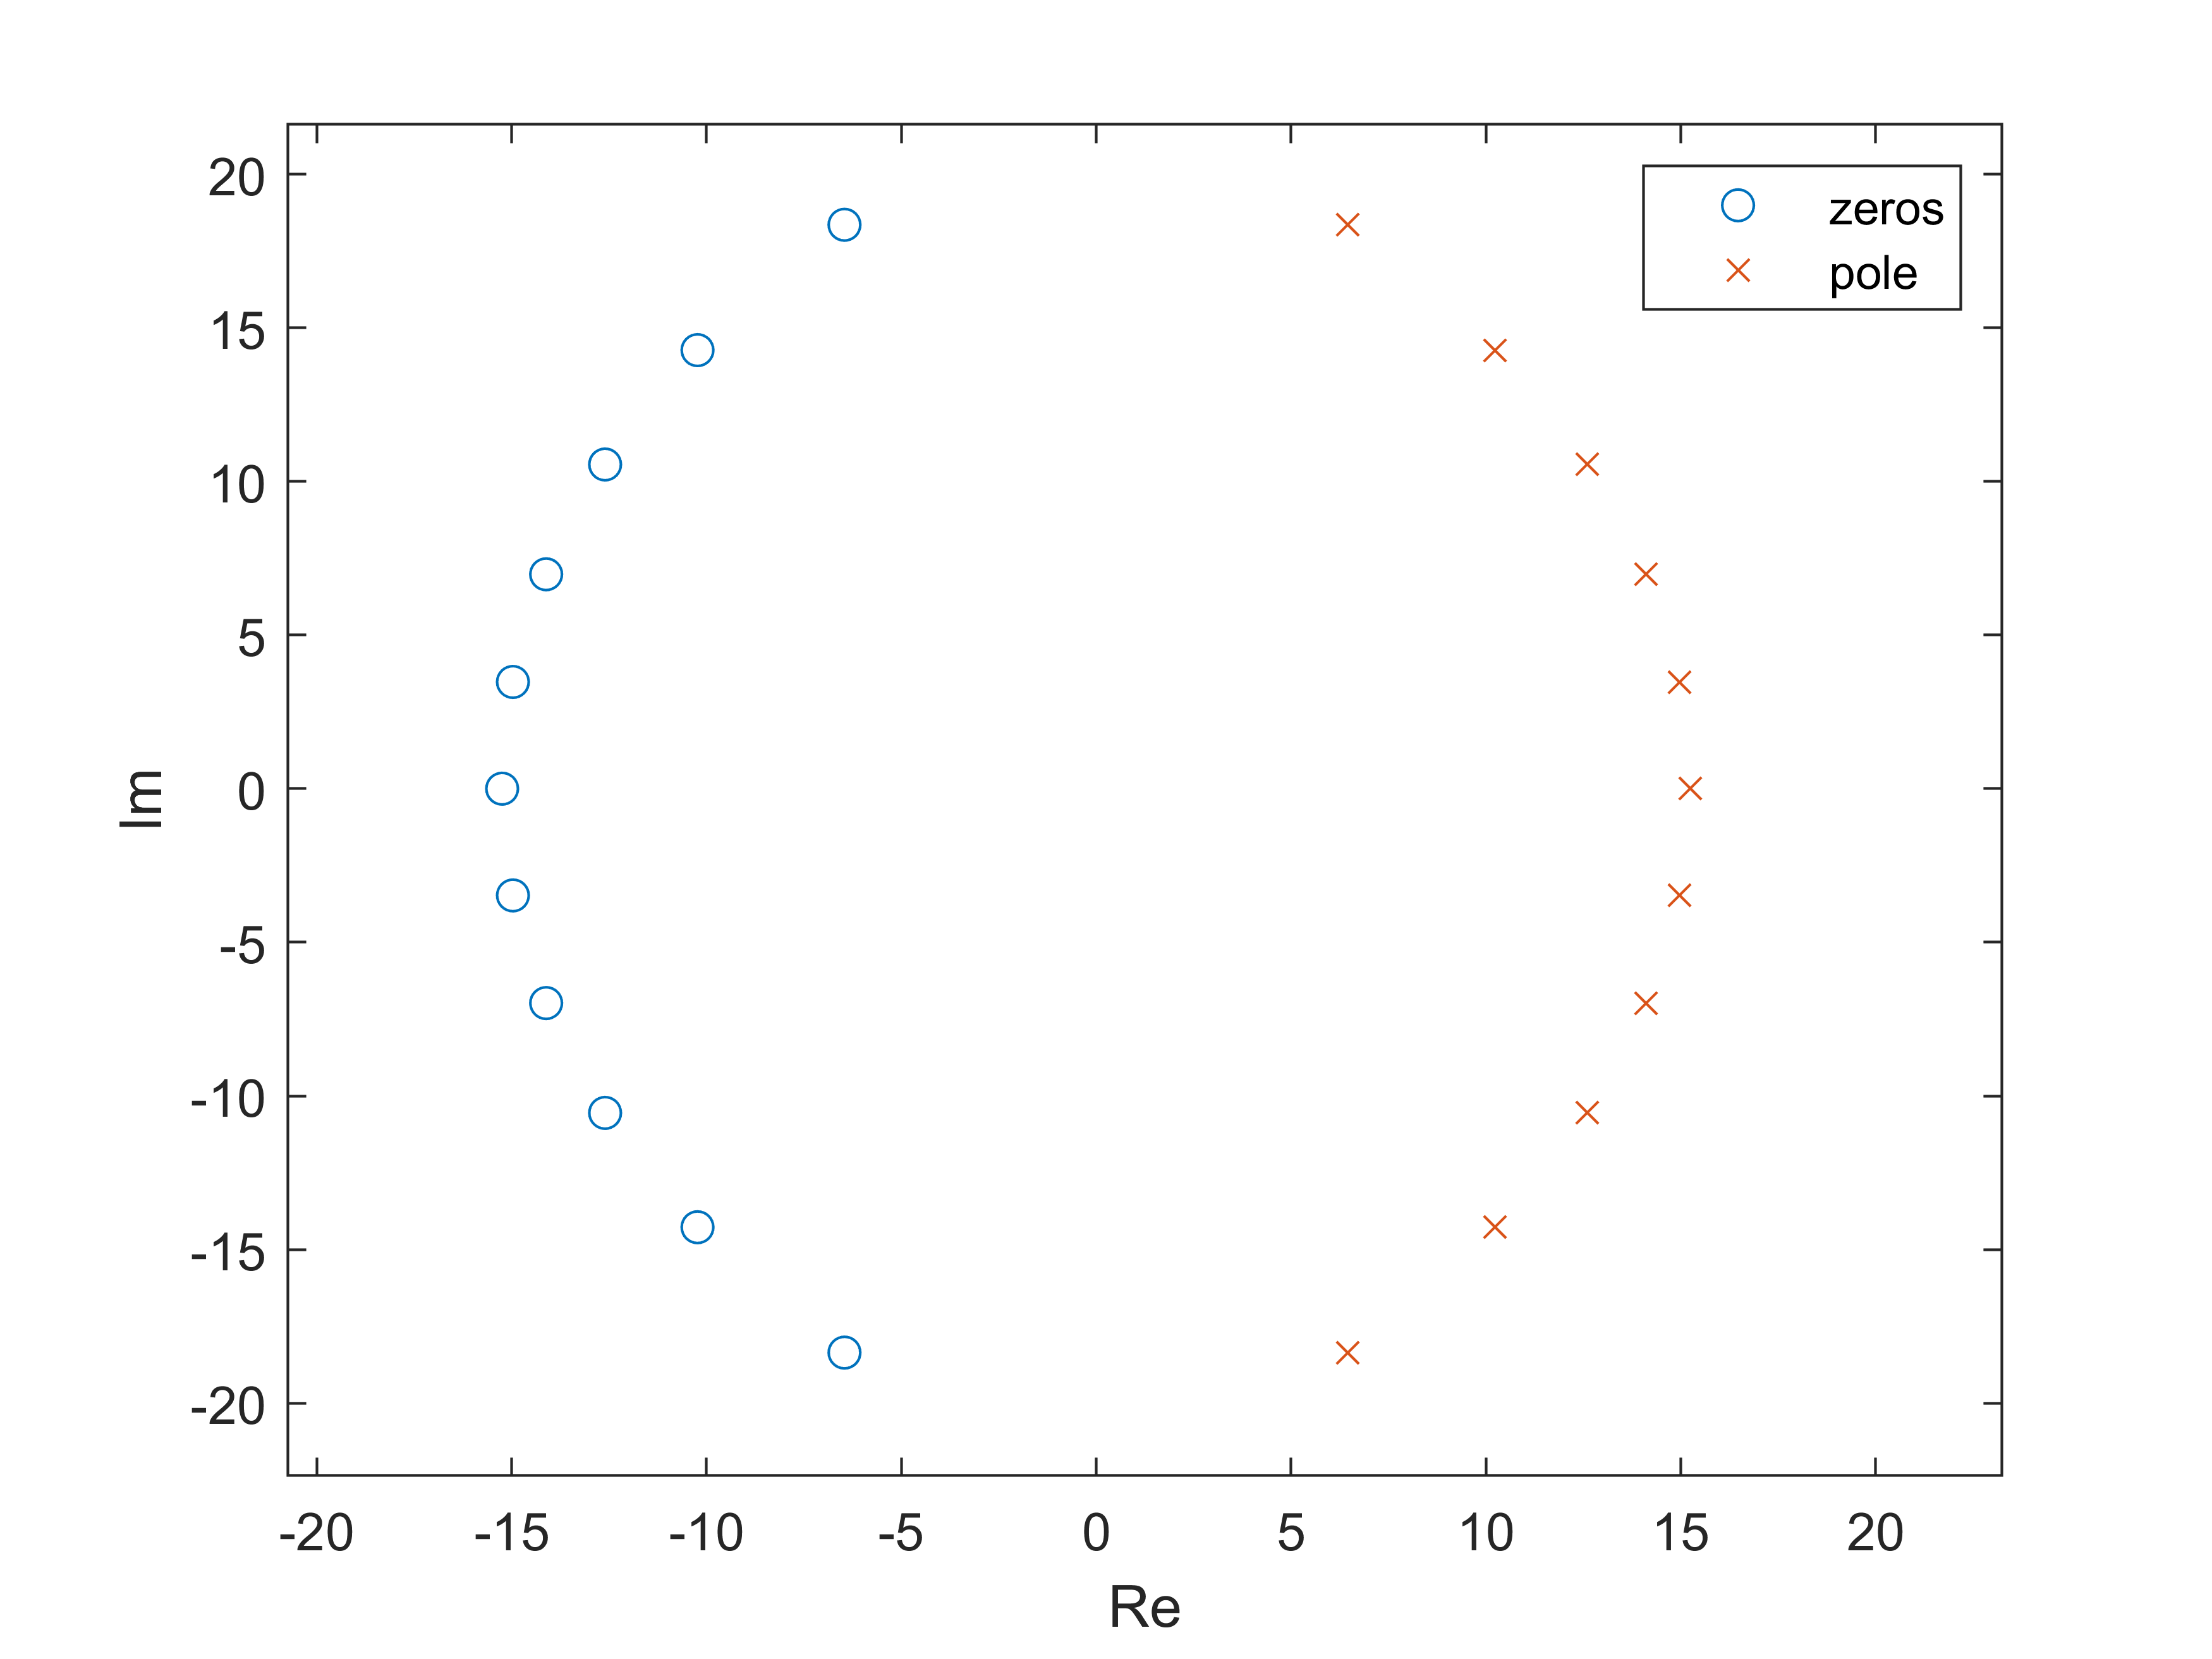
\includegraphics[width=\textwidth]{Files/q5,f4,11.png}
    \caption{Pole-Zero plot of $R_{11,11}(f_4)$}
        \end{minipage}
\end{figure}
\noindent All zeros lie have negative real part whereas all poles have positive real part. The zeros/poles are symmetric in the line $Im(z)=0$. This is because the zeros/poles come in conjugate pairs. They are aslo symmetric in the line $Re(z)=0$ such that if there is a zero at $(-x,y)$, then there is a pole at $(x,y)$.\\
As $L$ increases, the radial distance from the pole/zero to the origin increases, and the points remain in their shape of a pair of parabolas.\\\\

\noindent \textbf{With $f_5$}, we will now look at when $L=4,8,9,10$.
\begin{figure}[H]
    \begin{minipage}[b]{0.47\linewidth}
            \centering
            \textbf{L=4}\par
            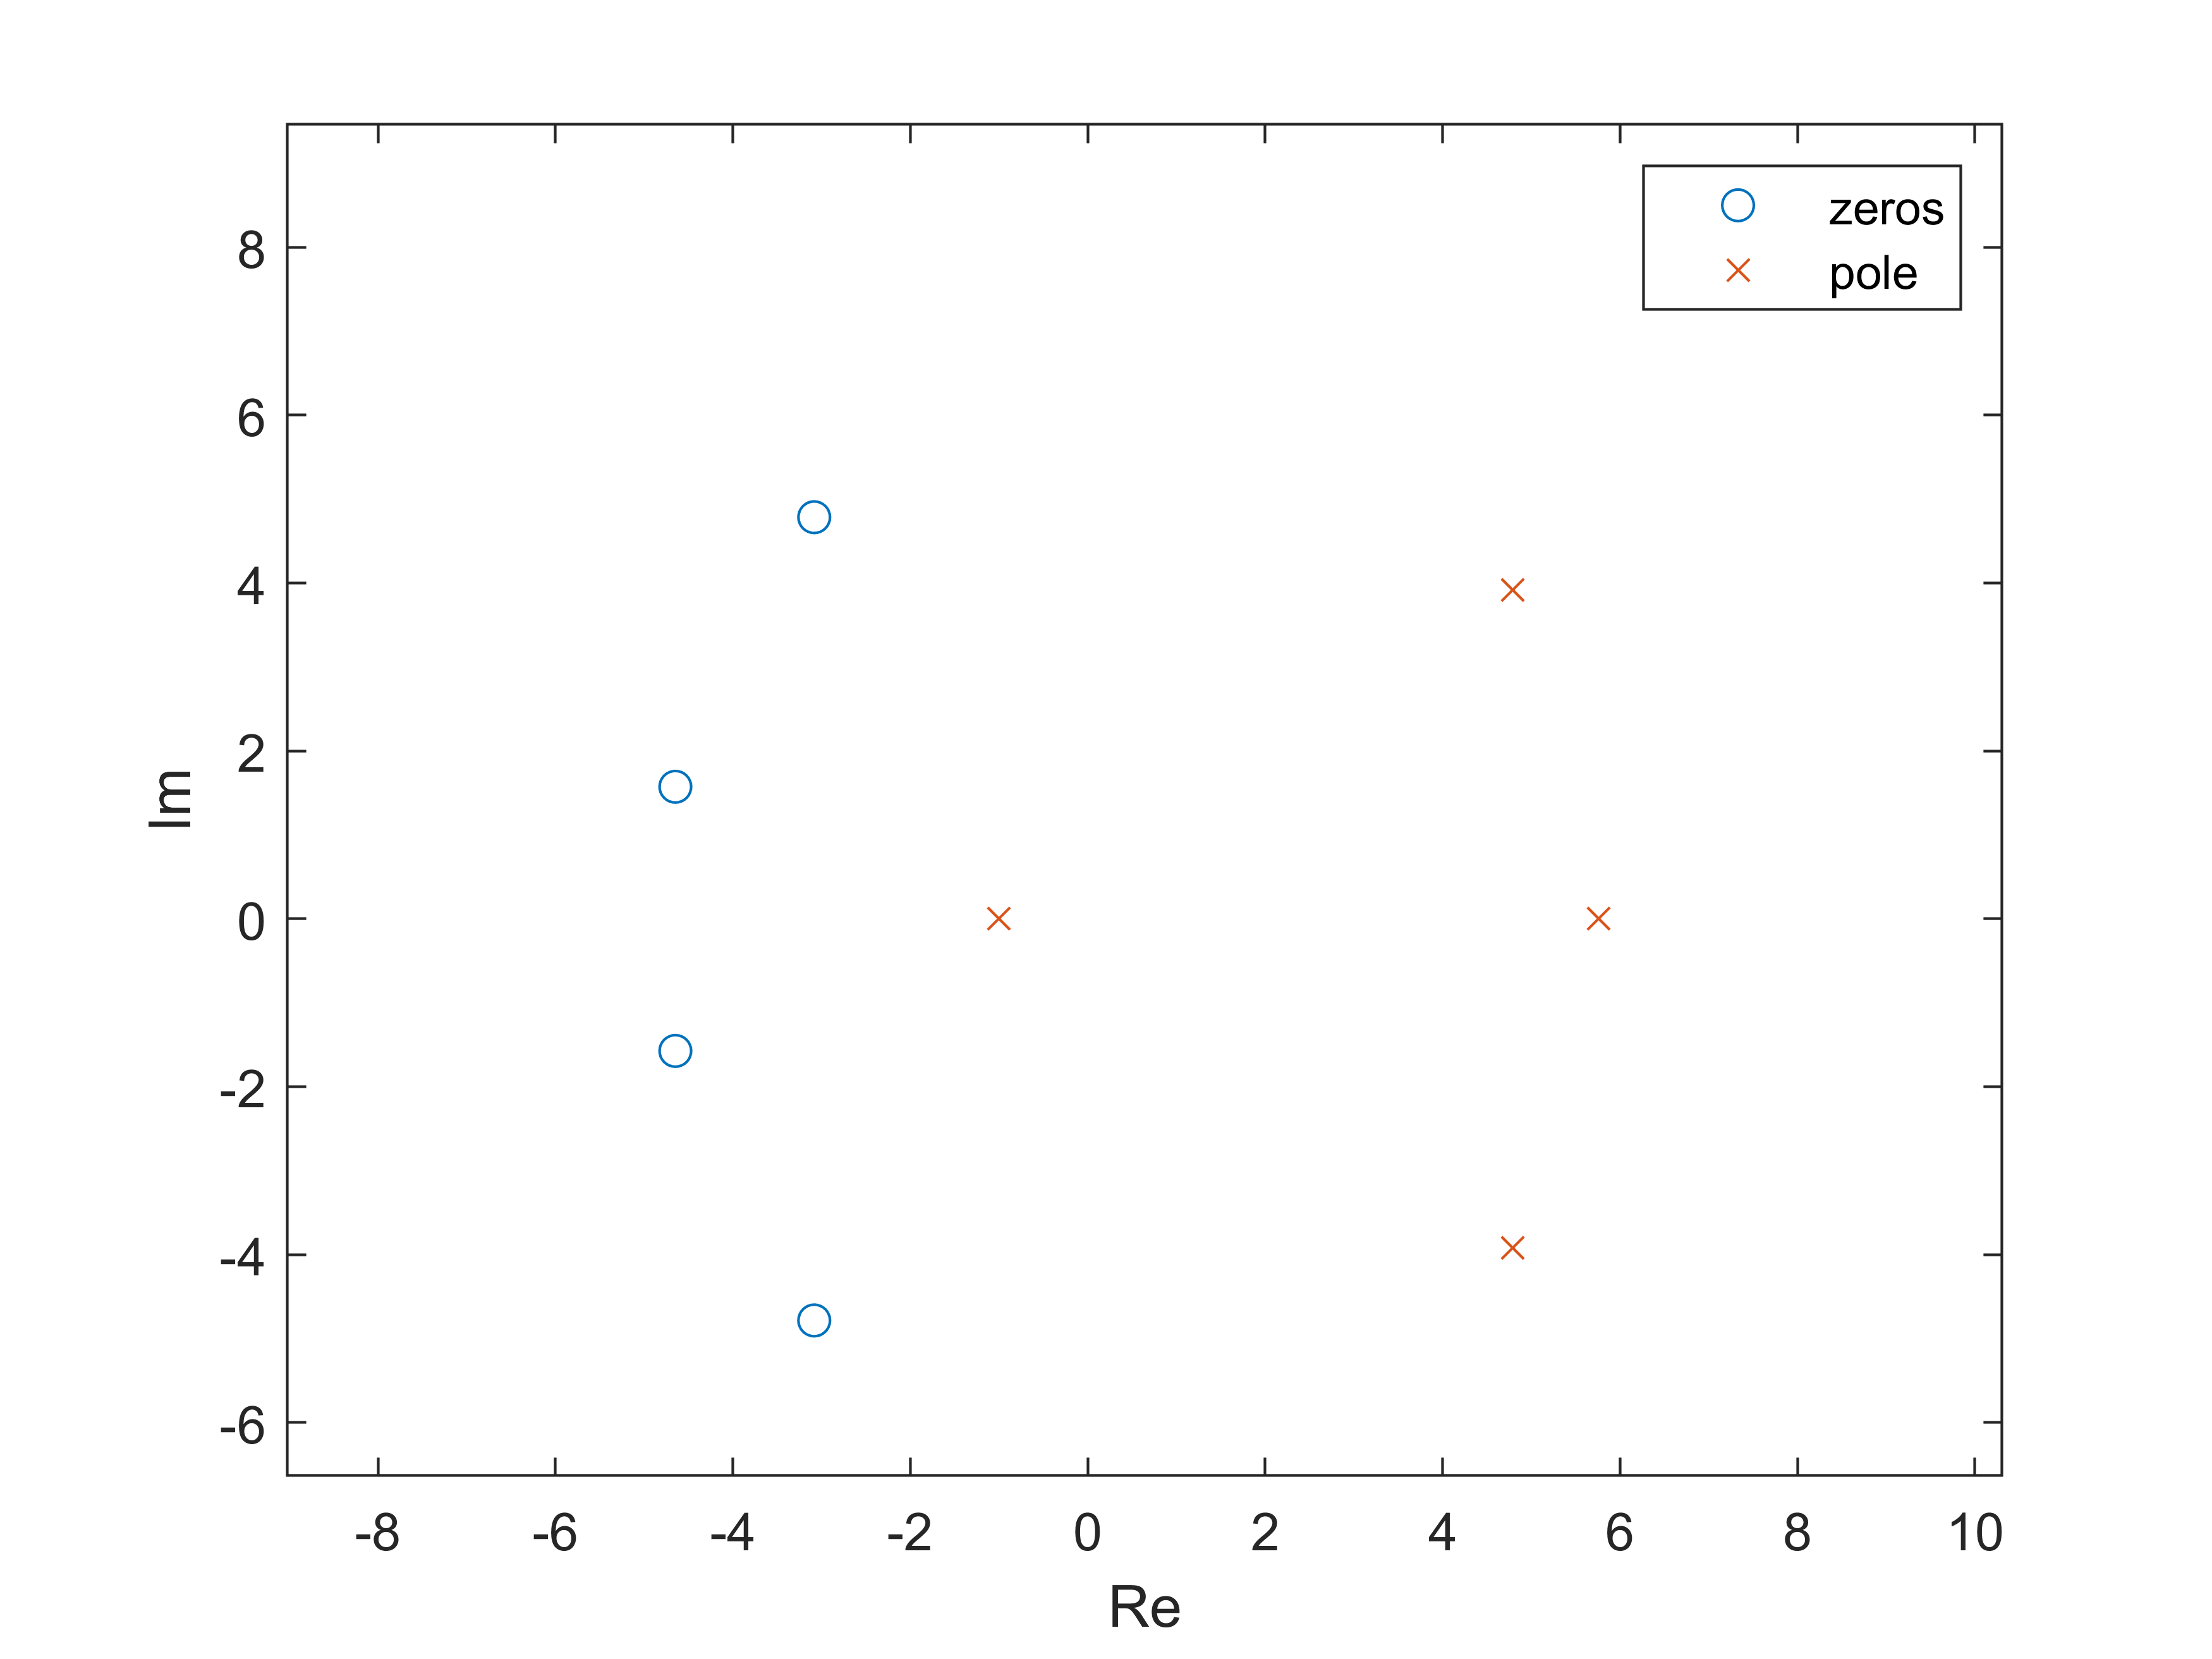
\includegraphics[width=\textwidth]{Files/q5,f5,4.png}
            \caption{Pole-Zero plot of $R_{4,4}(f_5)$}
        \end{minipage}
        \hfill
            \begin{minipage}[b]{0.47\linewidth}
            \centering
    \textbf{L=8}\par
    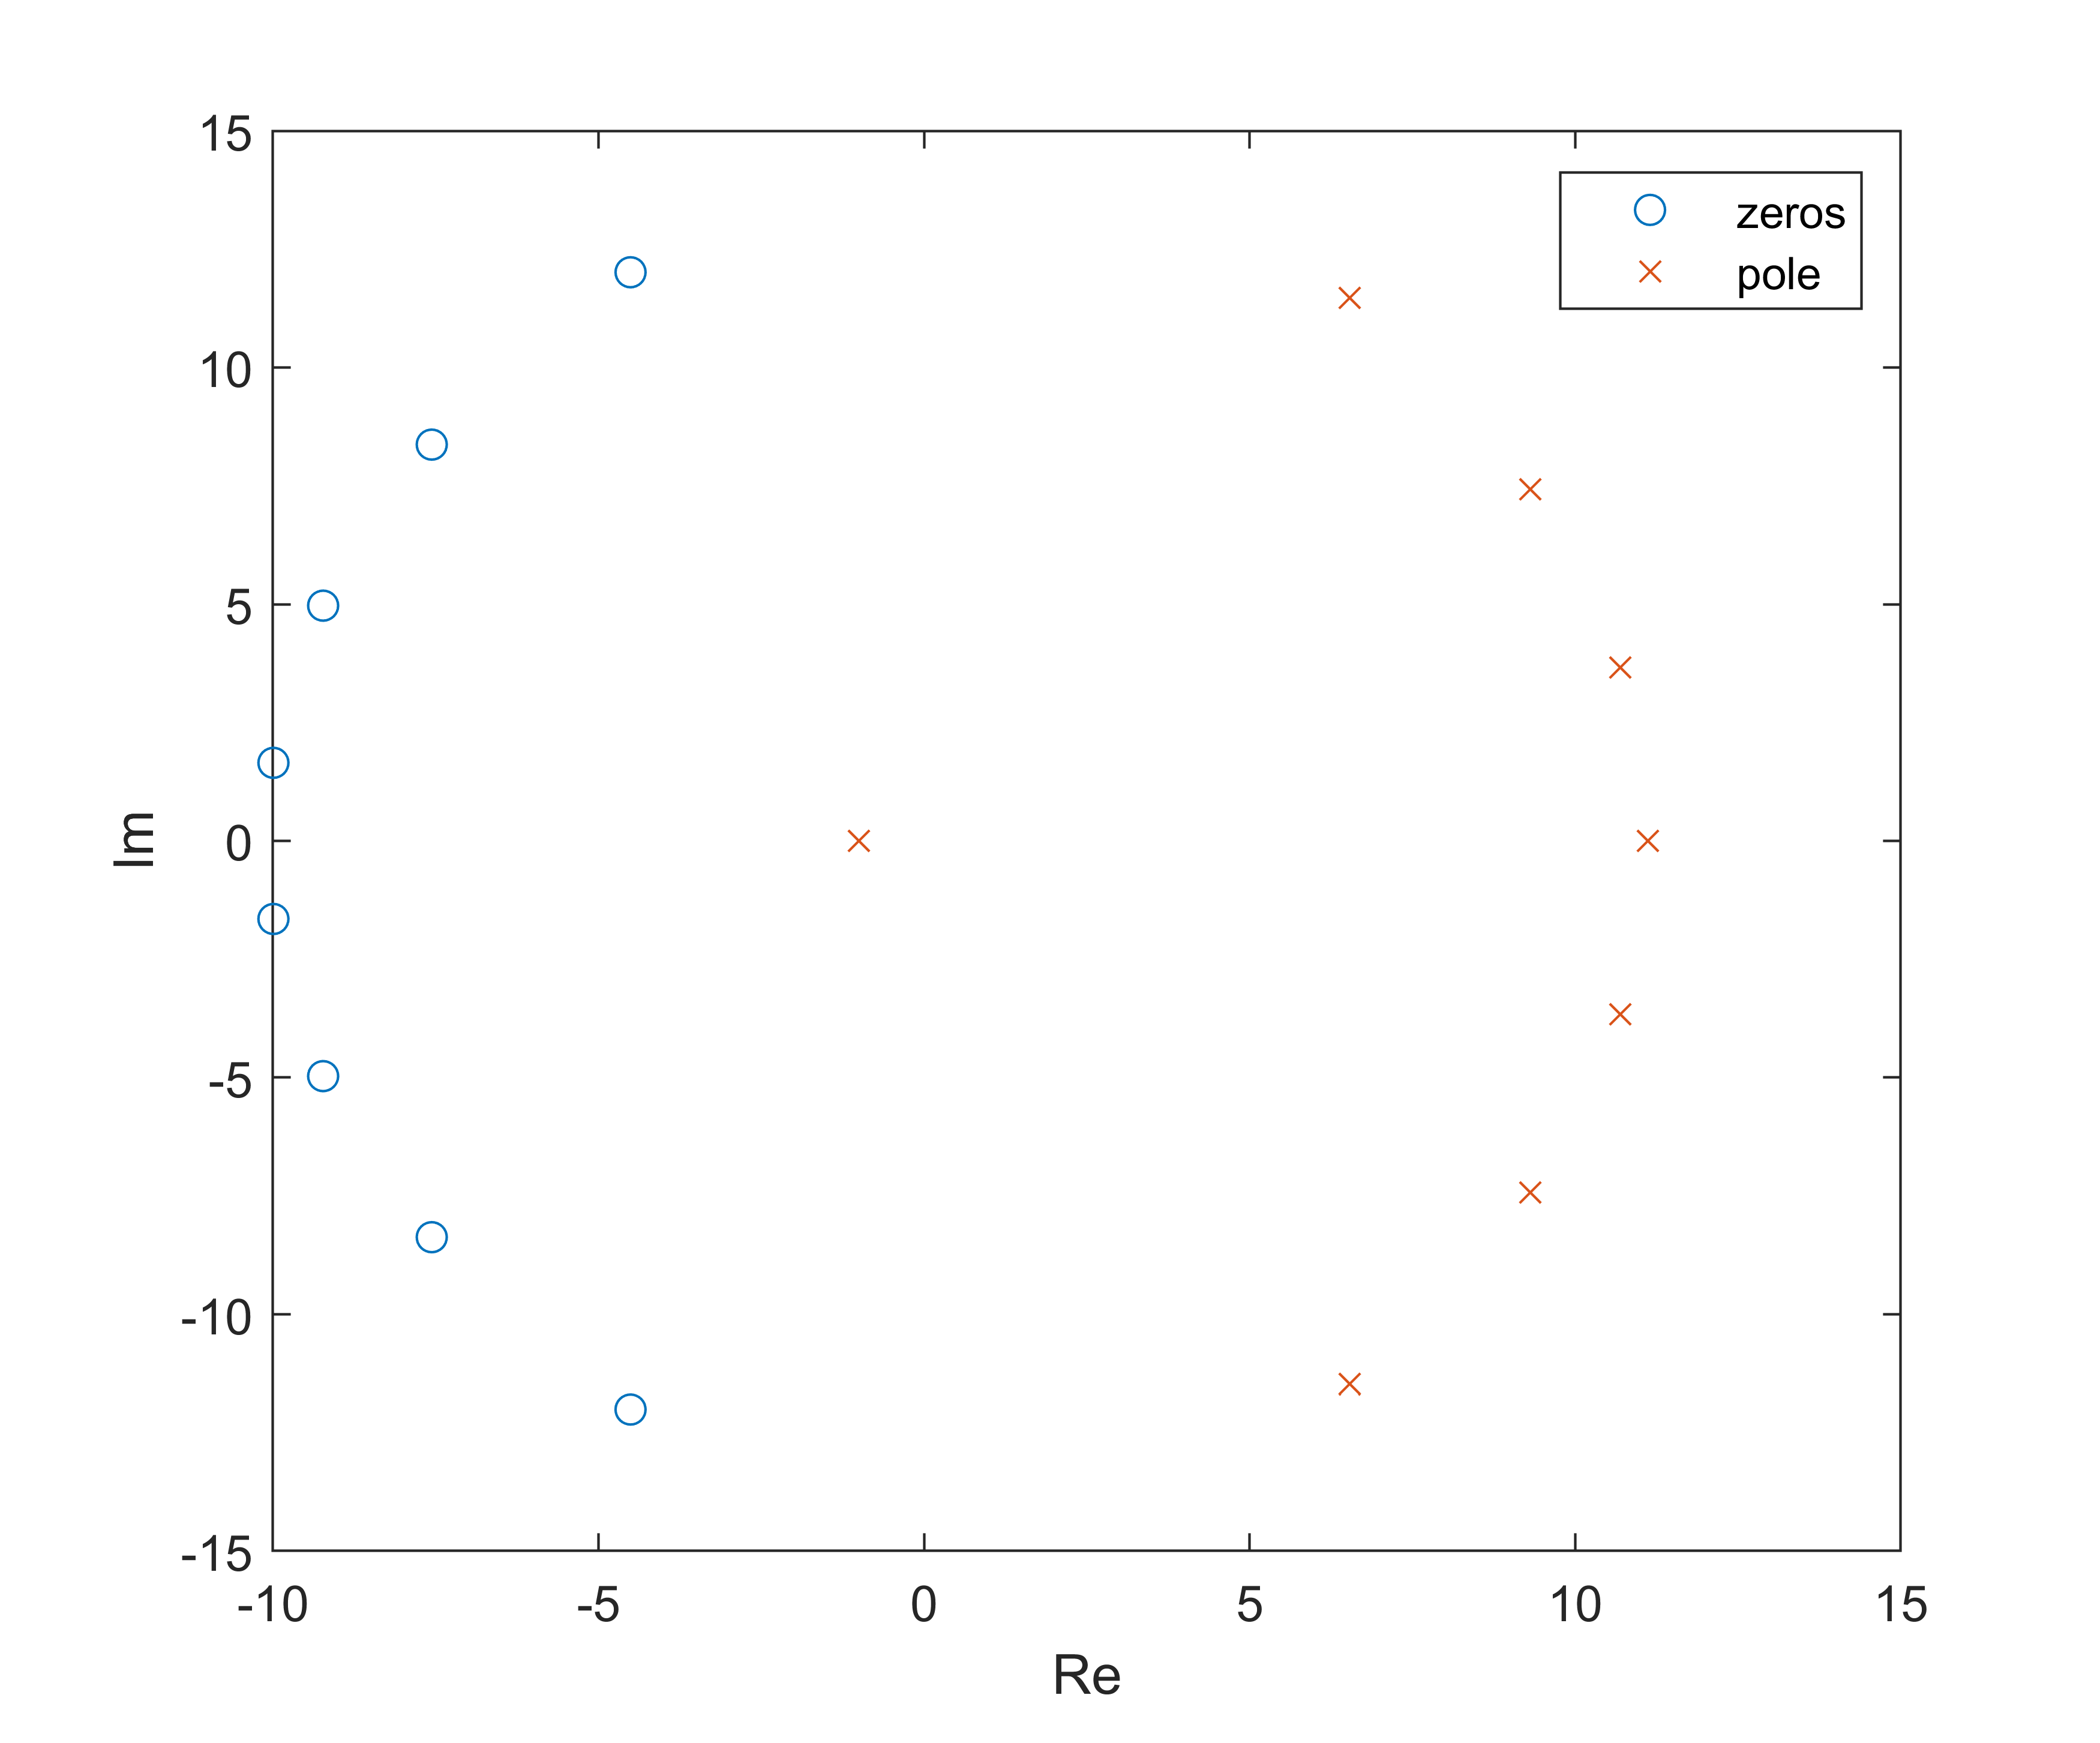
\includegraphics[width=\textwidth]{Files/q5,f5,8.png}
    \caption{Pole-Zero plot of $R_{8,8}(f_5)$}
        \end{minipage}
\end{figure}
\begin{figure}[H]
    \begin{minipage}[b]{0.47\linewidth}
            \centering
            \textbf{L=9}\par
            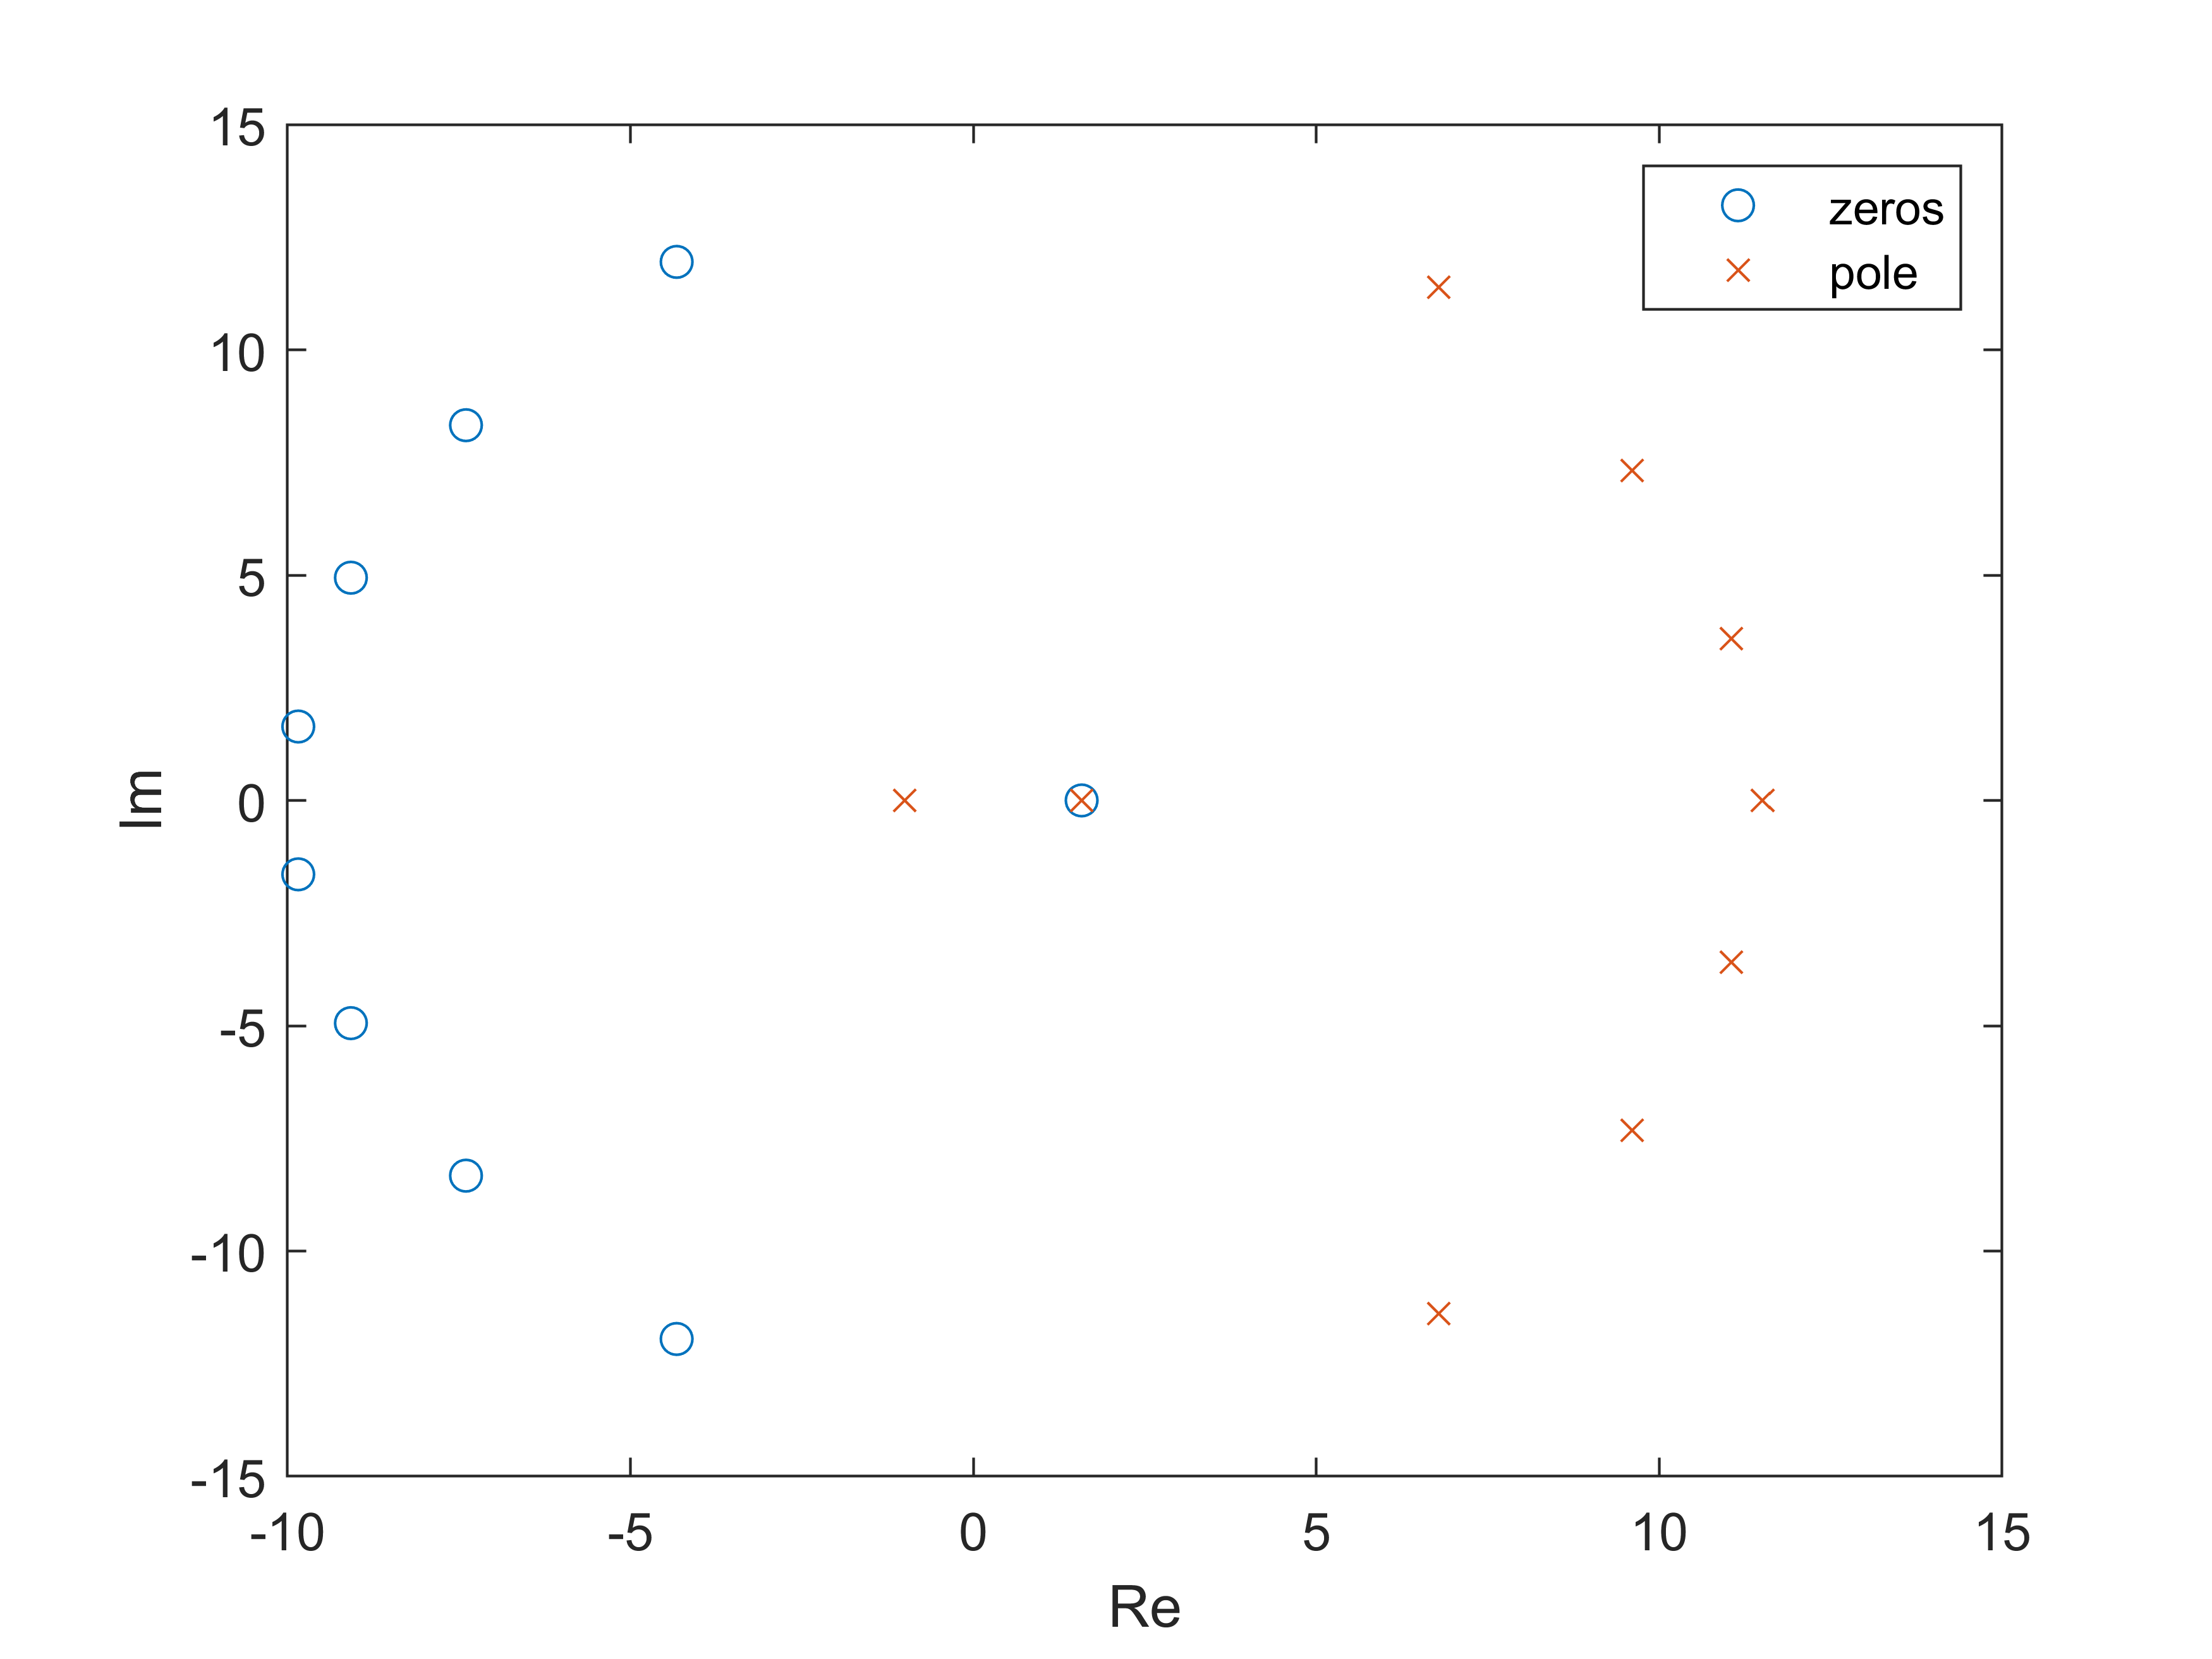
\includegraphics[width=\textwidth]{Files/q5,f5,9.png}
            \caption{Pole-Zero plot of $R_{9,9}(f_5)$}
        \end{minipage}
        \hfill
            \begin{minipage}[b]{0.47\linewidth}
            \centering
    \textbf{L=10}\par
    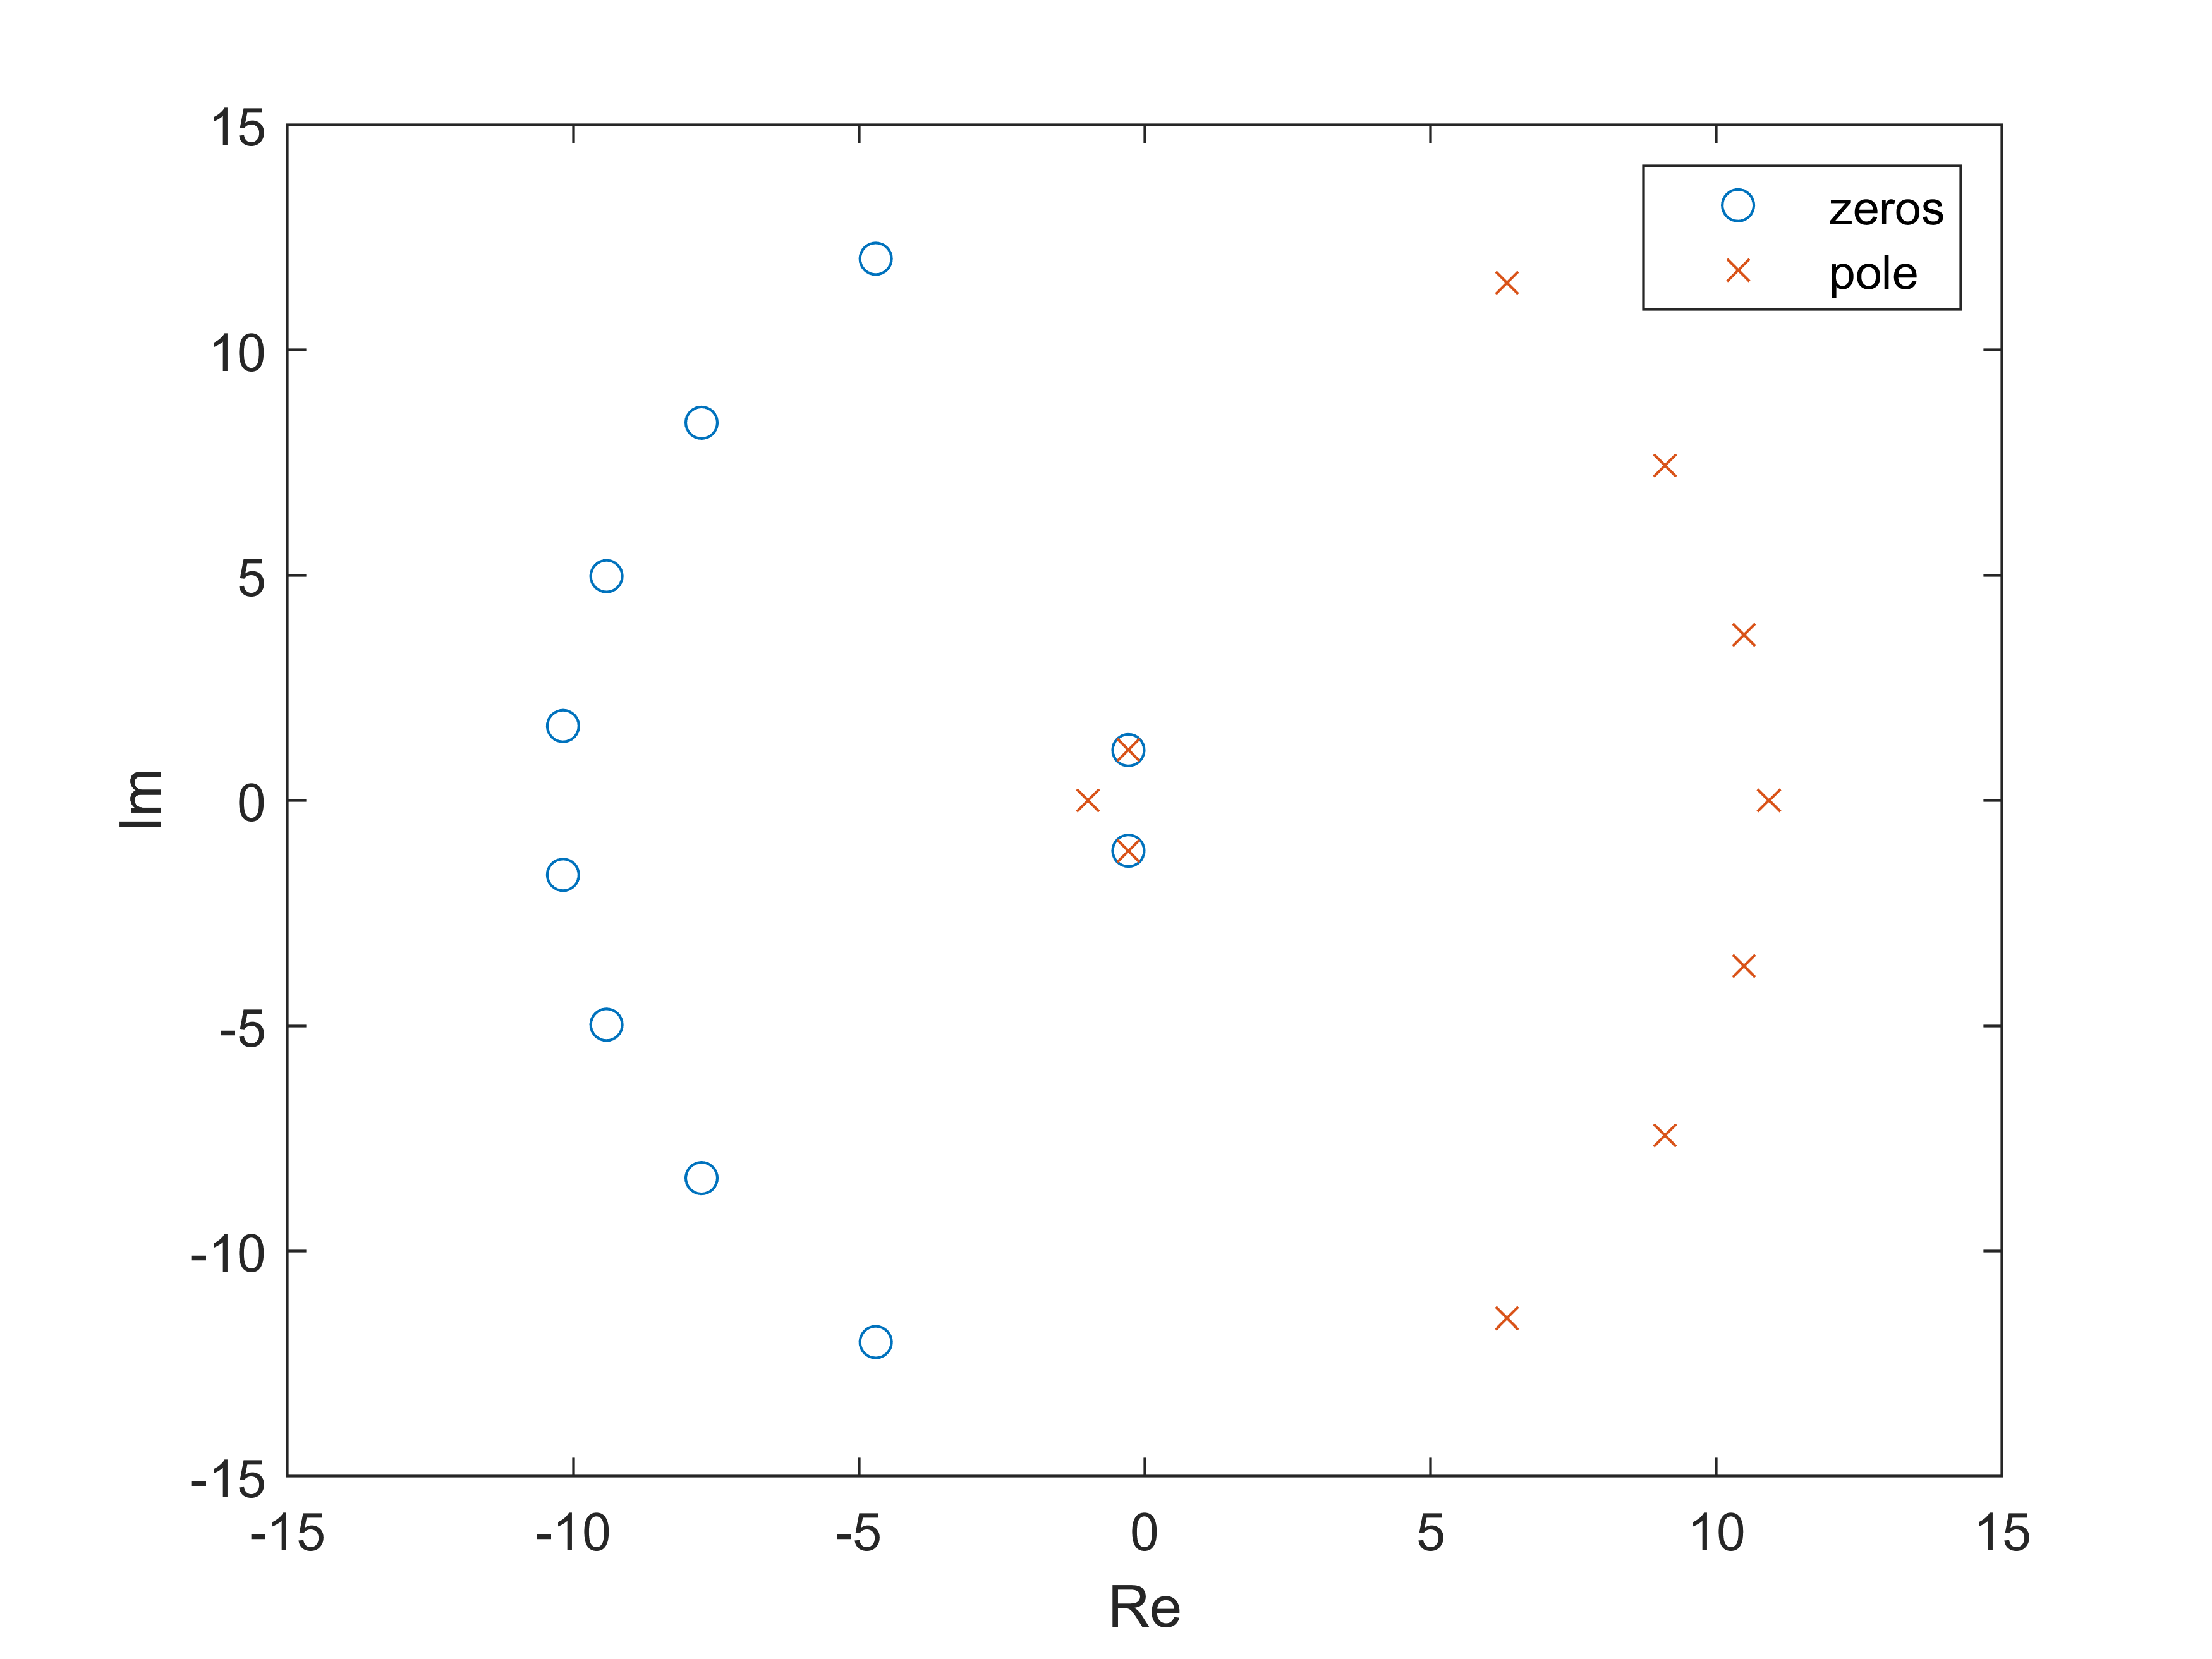
\includegraphics[width=\textwidth]{Files/q5,f5,10.png}
    \caption{Pole-Zero plot of $R_{10,10}(f_5)$}
        \end{minipage}
\end{figure}
\noindent For all $L$, there exists a pole at $(-1,0)$. Initially, when $L$ is small, e.g. from $L=4$ to figure $L=8$, the positions change similarly to those of $f_4$, such that the zeros are on the left half plane and the poles are all the right half plane except the one pole at $(-1,0)$. However, as $L$ increases, e.g. from $8$ to $9$ and then $10$, no new zeros/poles are introduced onto the pair of parabolas we saw in $R_{L,L}(f_4)$, instead, the new zero/pole overlap each other and are conjugate to one other zero/pole introduced this way.This implies that is no new pole or zero as $L$ increases, since these factors will cancel out.\\\\
\\\\
Finally, \textbf{for $f_6$}, we will look at $L=7,8$.
\begin{figure}[H]
    \begin{minipage}[b]{0.47\linewidth}
            \centering
            \textbf{L=7}\par
            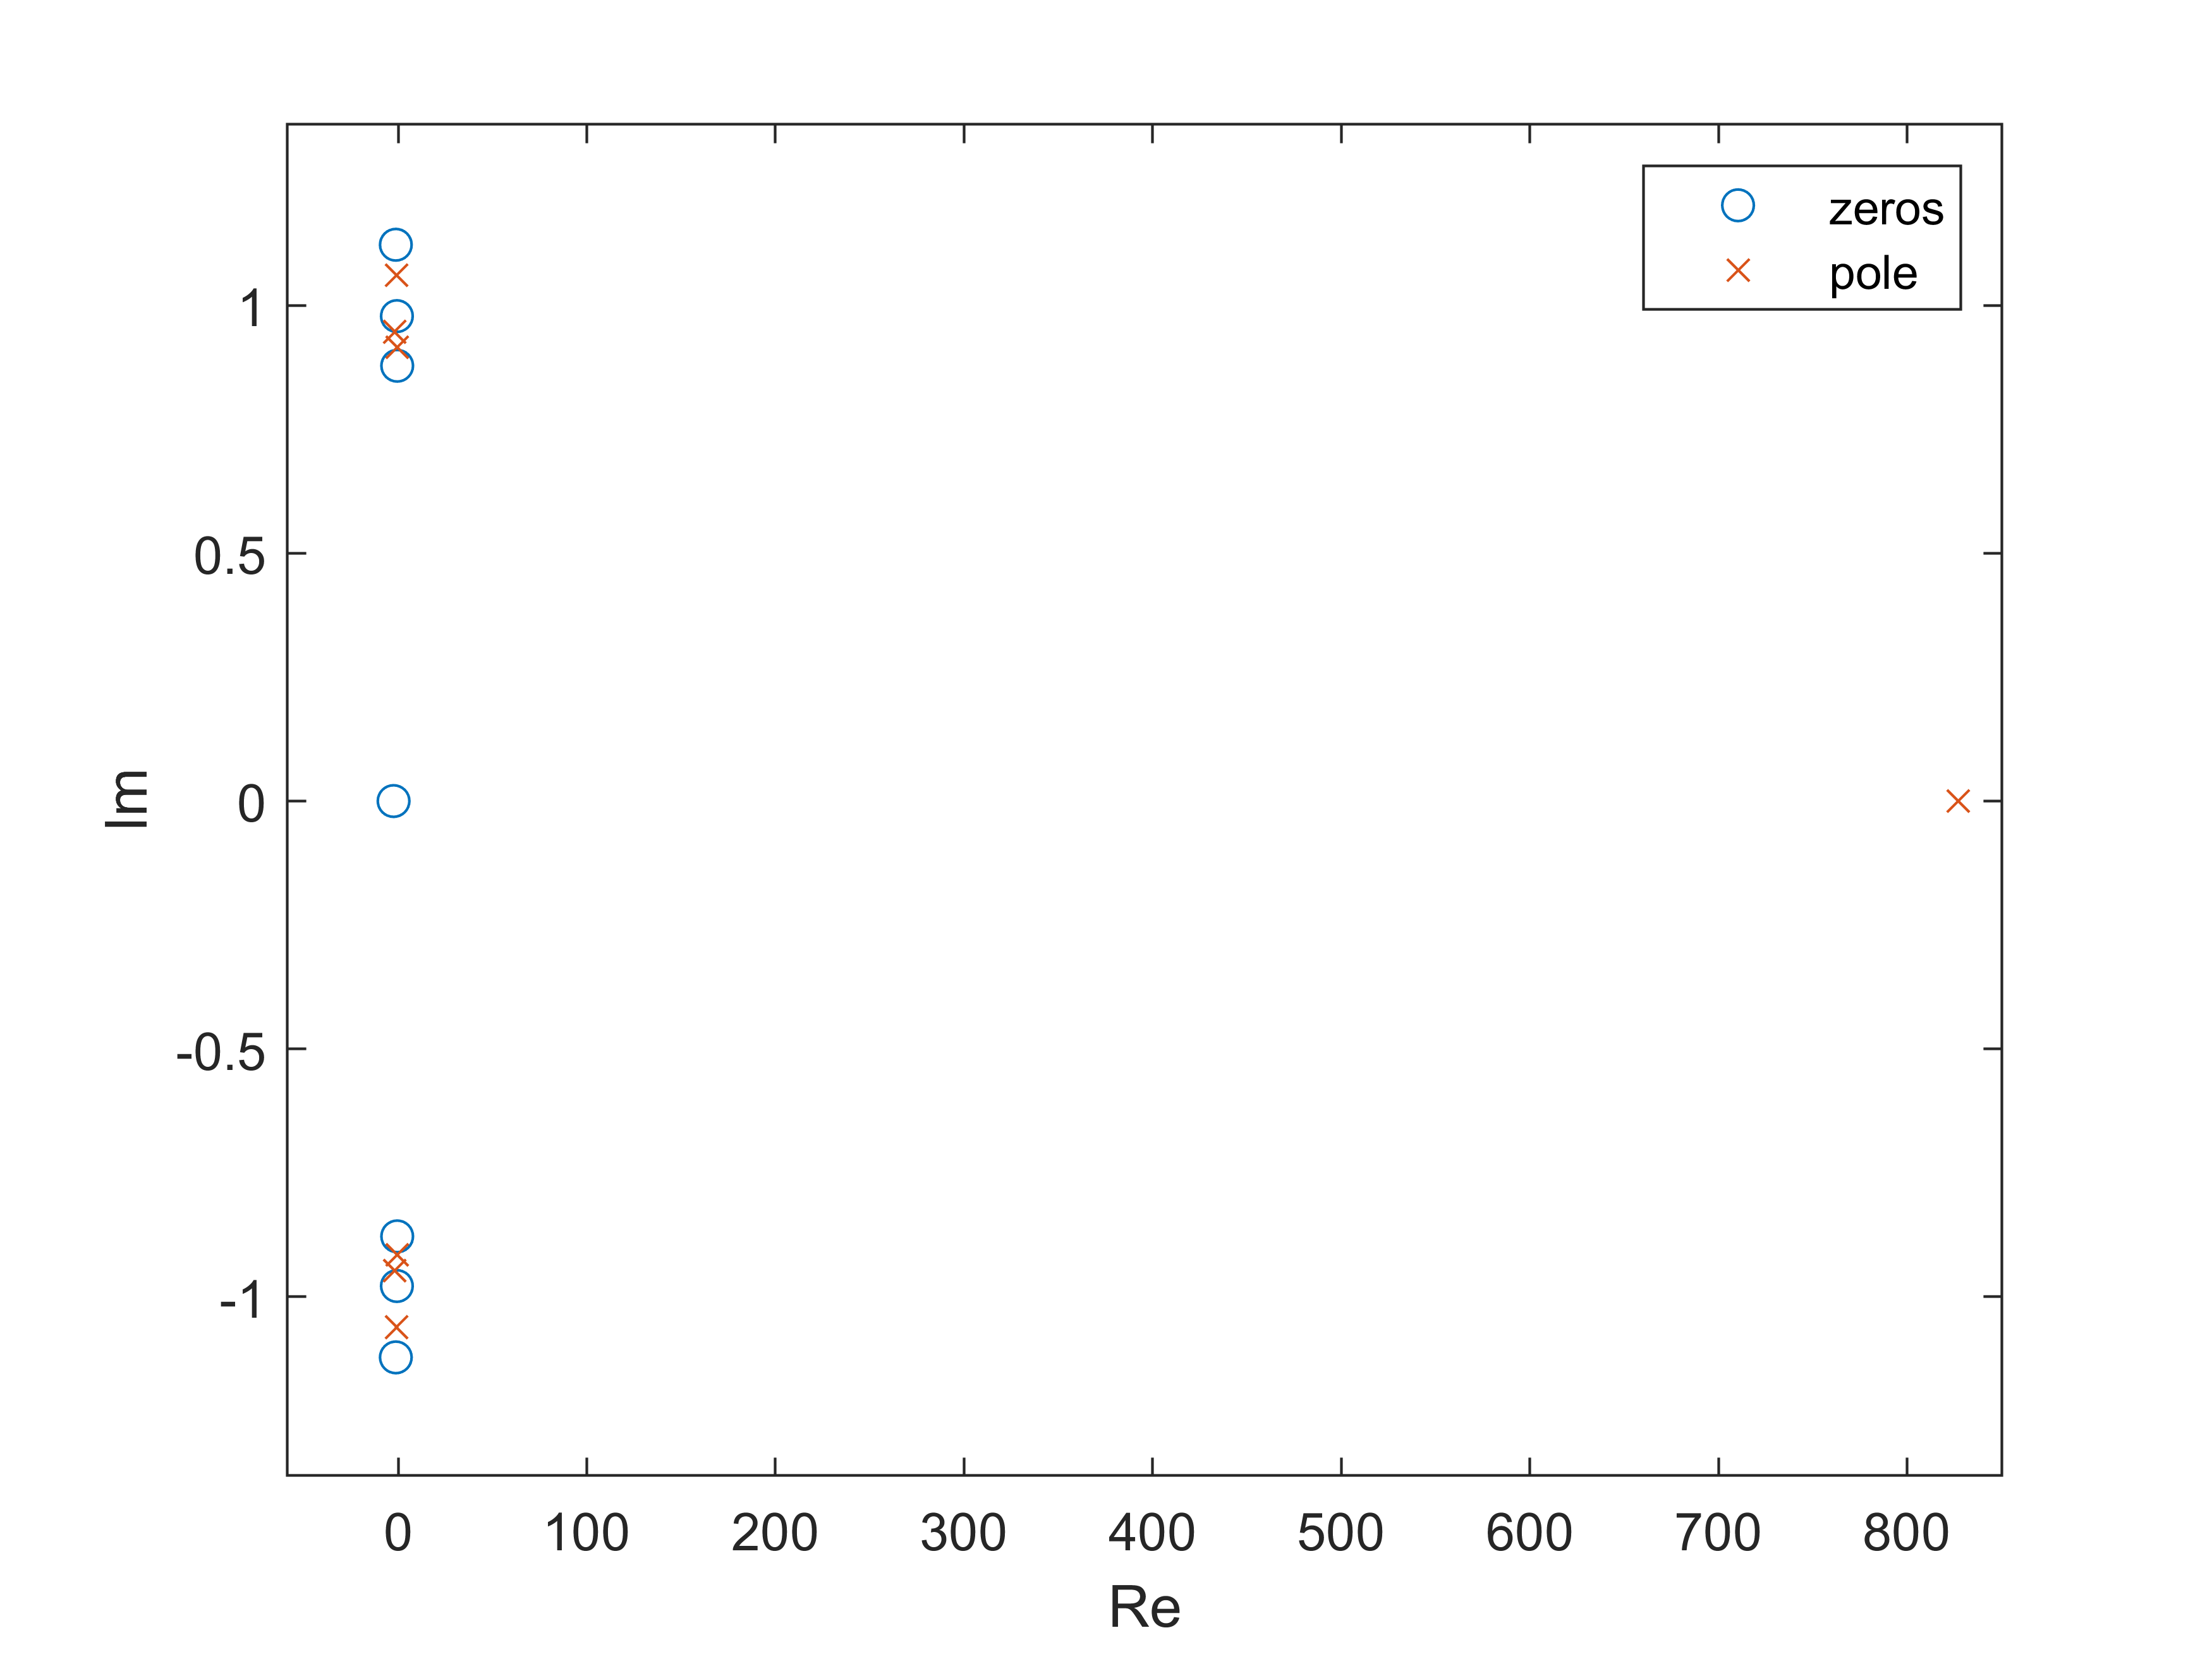
\includegraphics[width=\textwidth]{Files/q5,f6,7.png}
            \caption{Pole-Zero plot of $R_{7,7}(f_6)$}
        \end{minipage}
        \hfill
            \begin{minipage}[b]{0.47\linewidth}
            \centering
    \textbf{L=7,$Re(z)>-5$}\par
    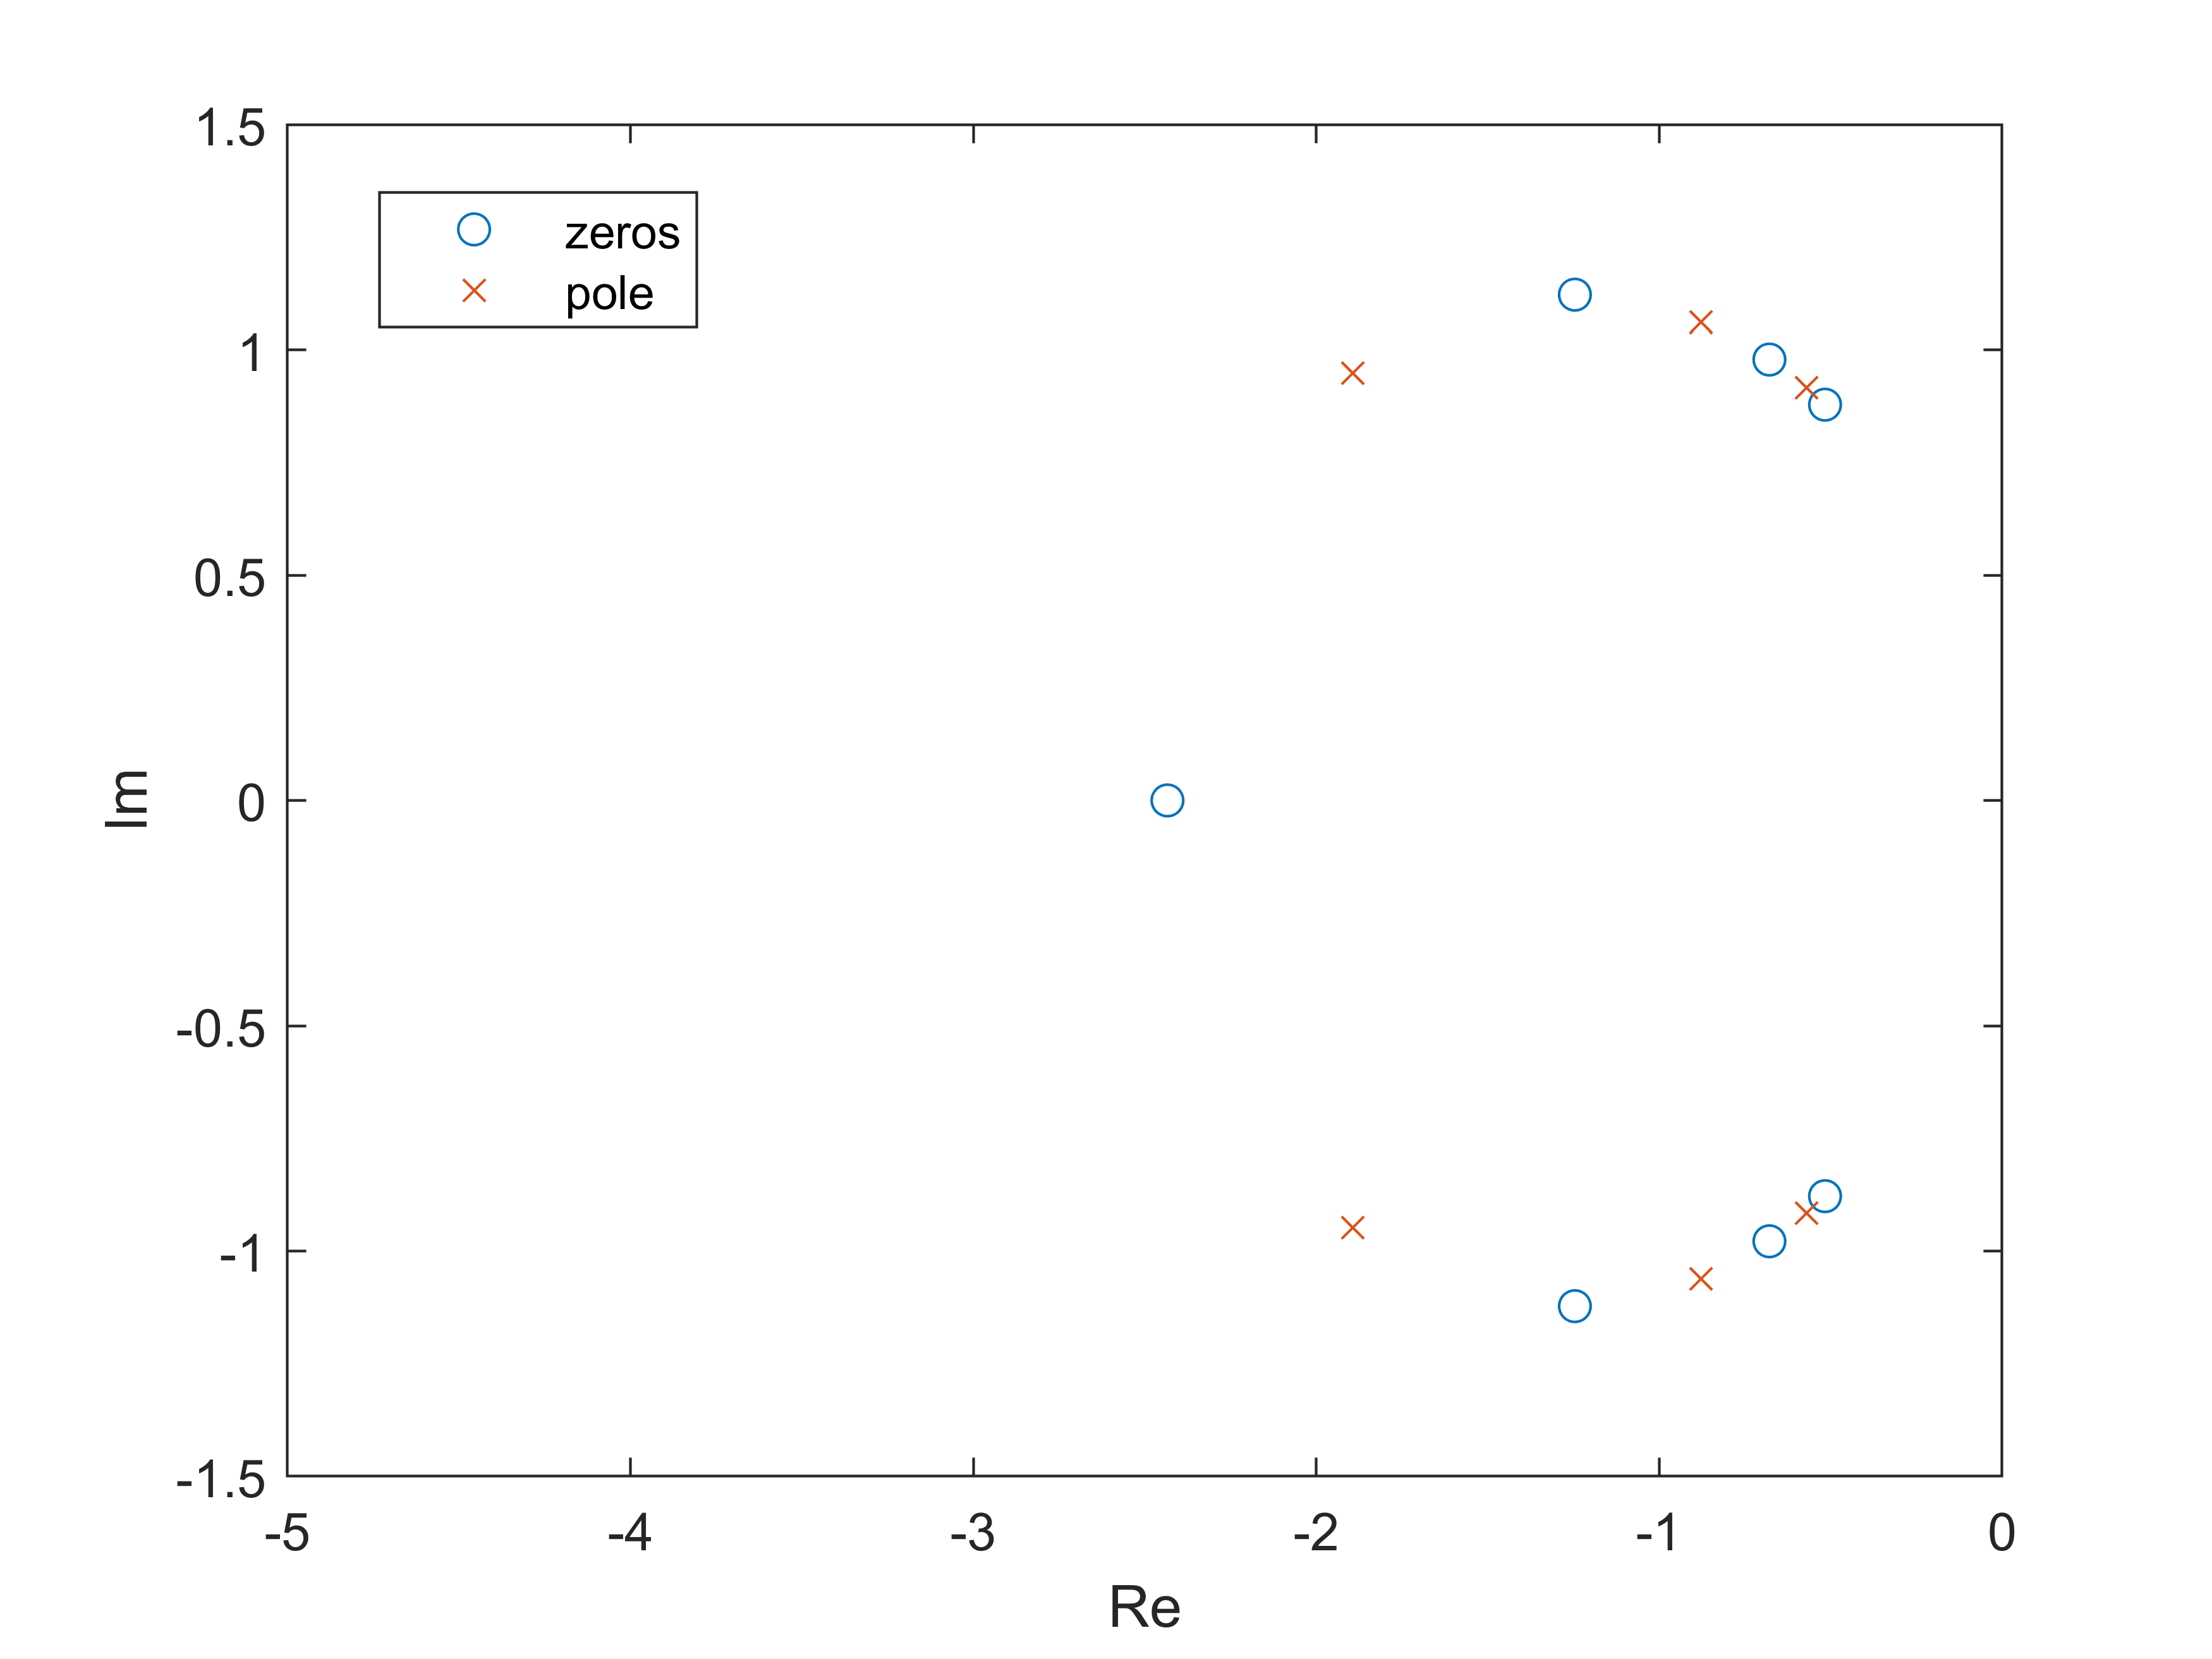
\includegraphics[width=\textwidth]{Files/q5,f6,7_ring.png}
    \caption{Pole-Zero plot of $R_{7,7}(f_6)$ near origin}
        \end{minipage}
\end{figure}
\begin{figure}[H]
    \begin{minipage}[b]{0.47\linewidth}
            \centering
            \textbf{L=8, }\par
            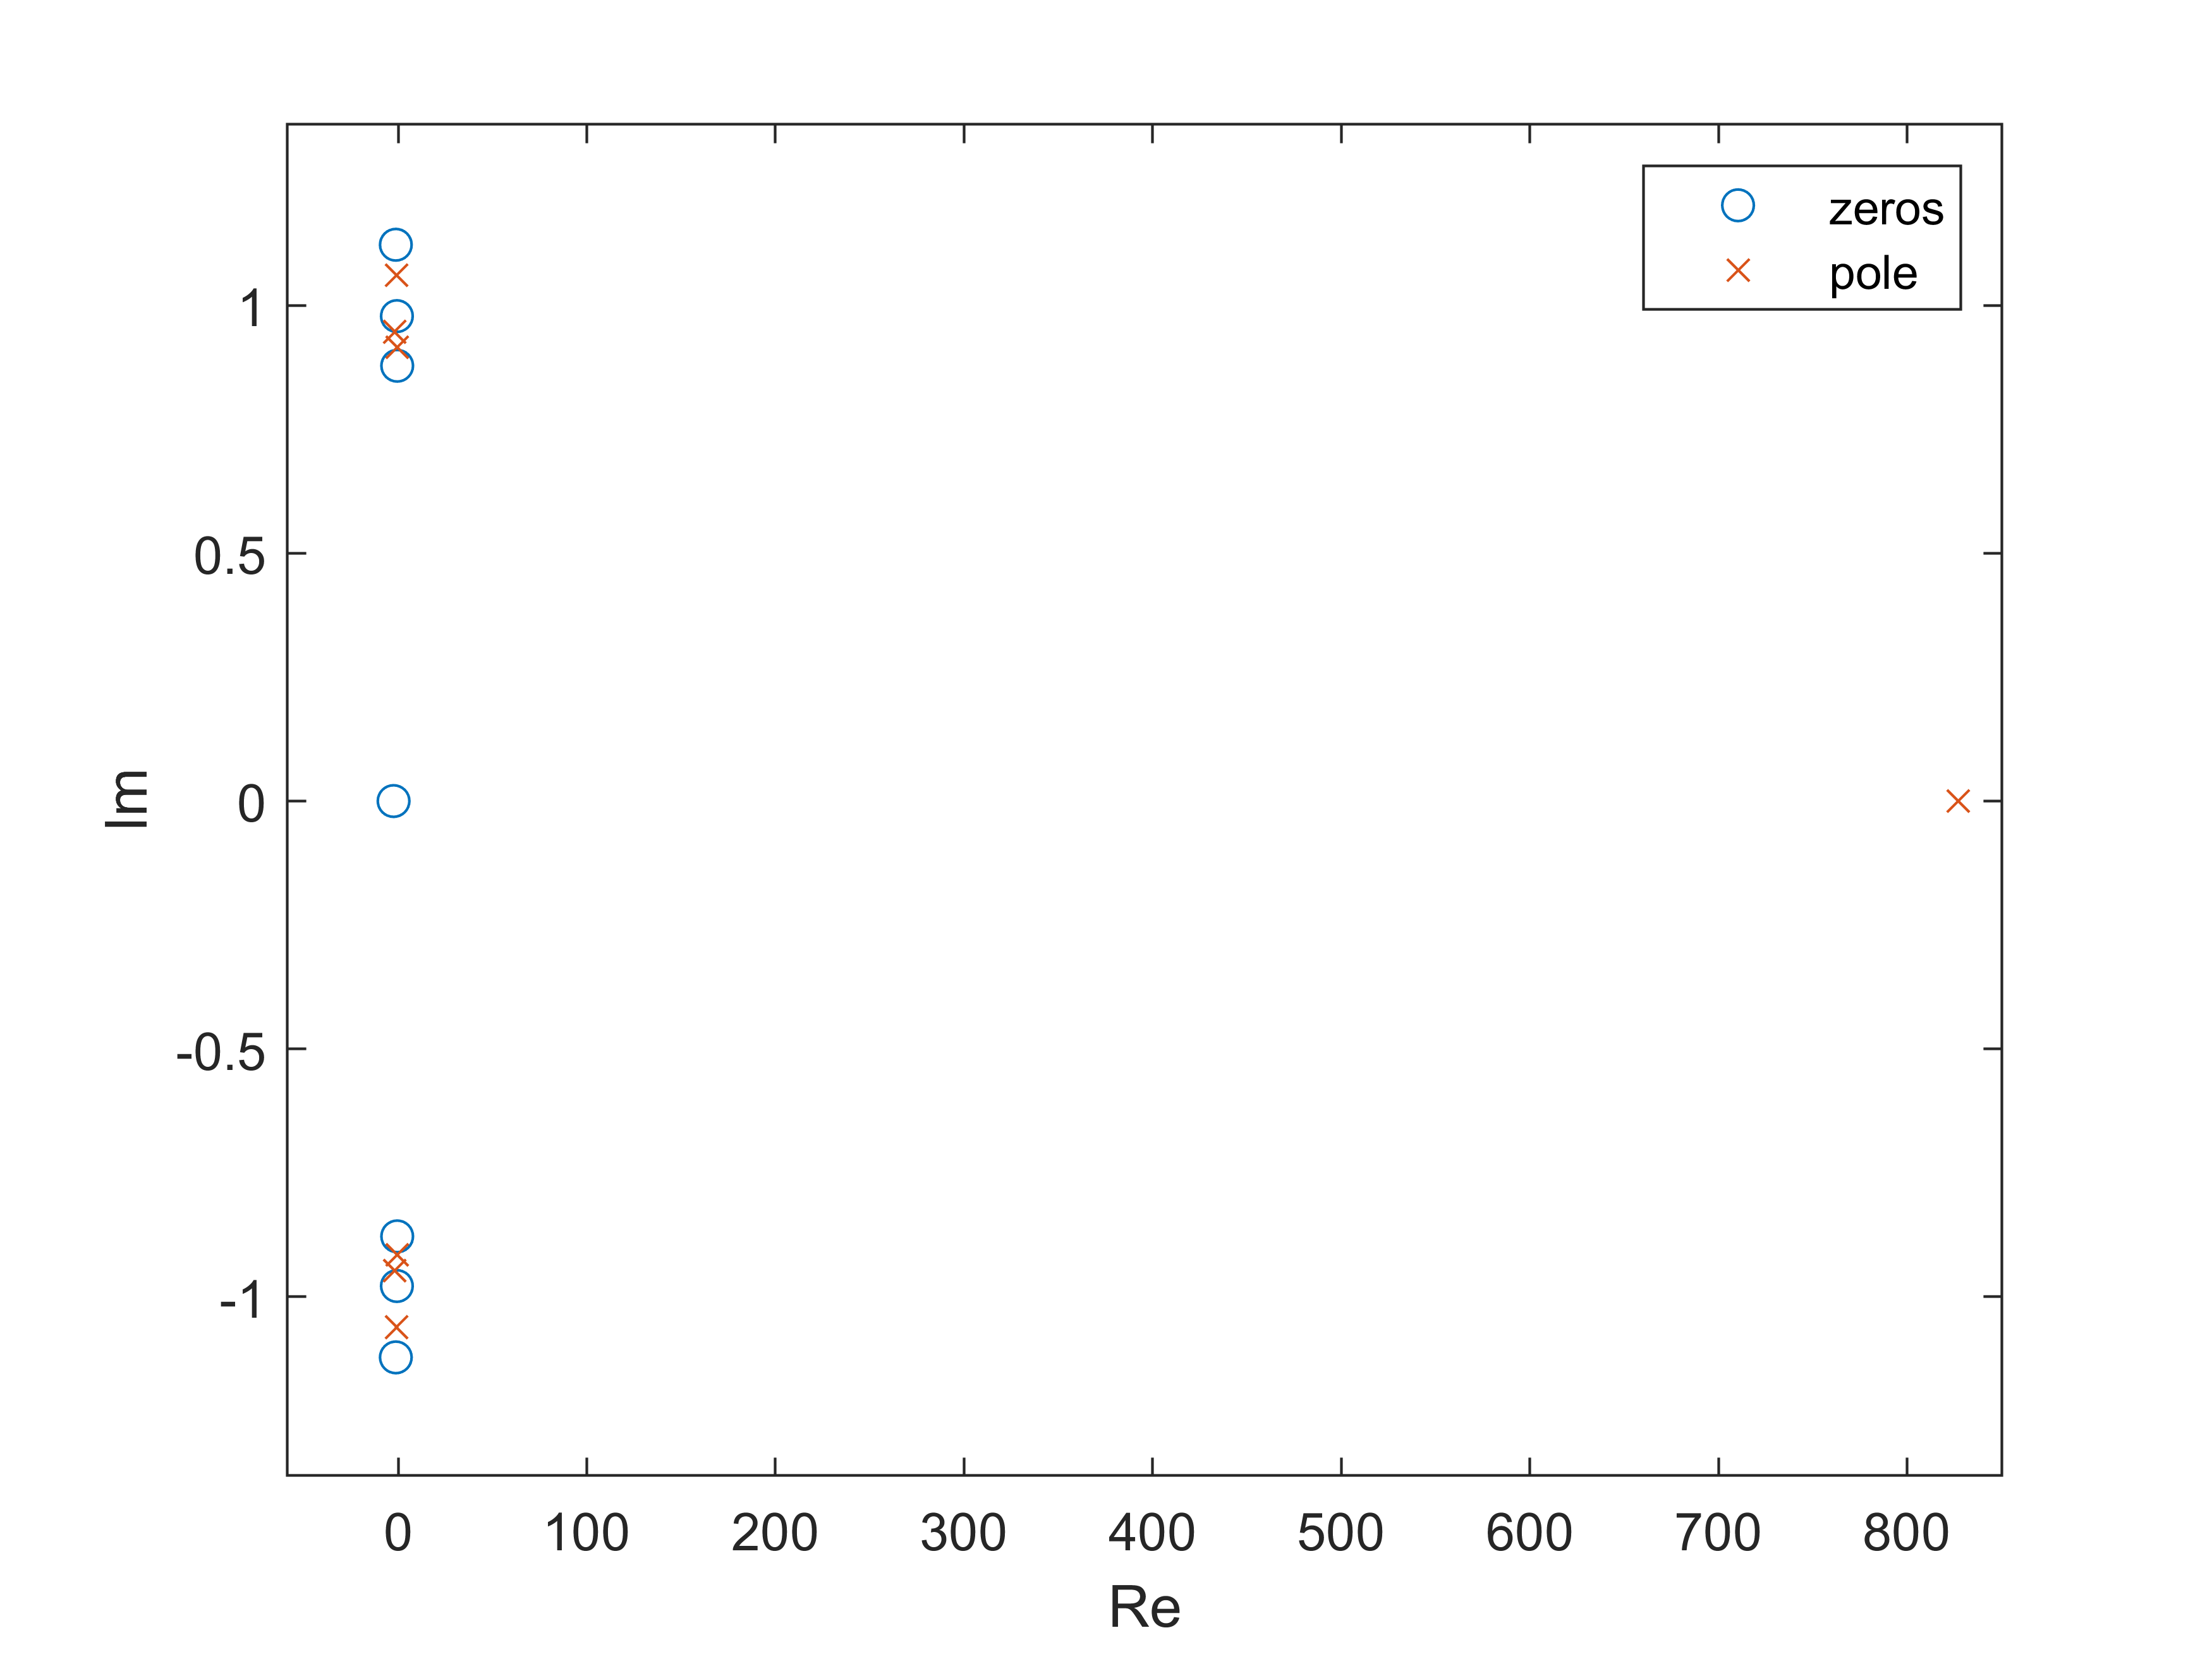
\includegraphics[width=\textwidth]{Files/q5,f6,7.png}
            \caption{Pole-Zero plot of $R_{8,8}(f_6)$}
        \end{minipage}
        \hfill
            \begin{minipage}[b]{0.47\linewidth}
            \centering
    \textbf{L=8, $Re(z)>-5$}\par
    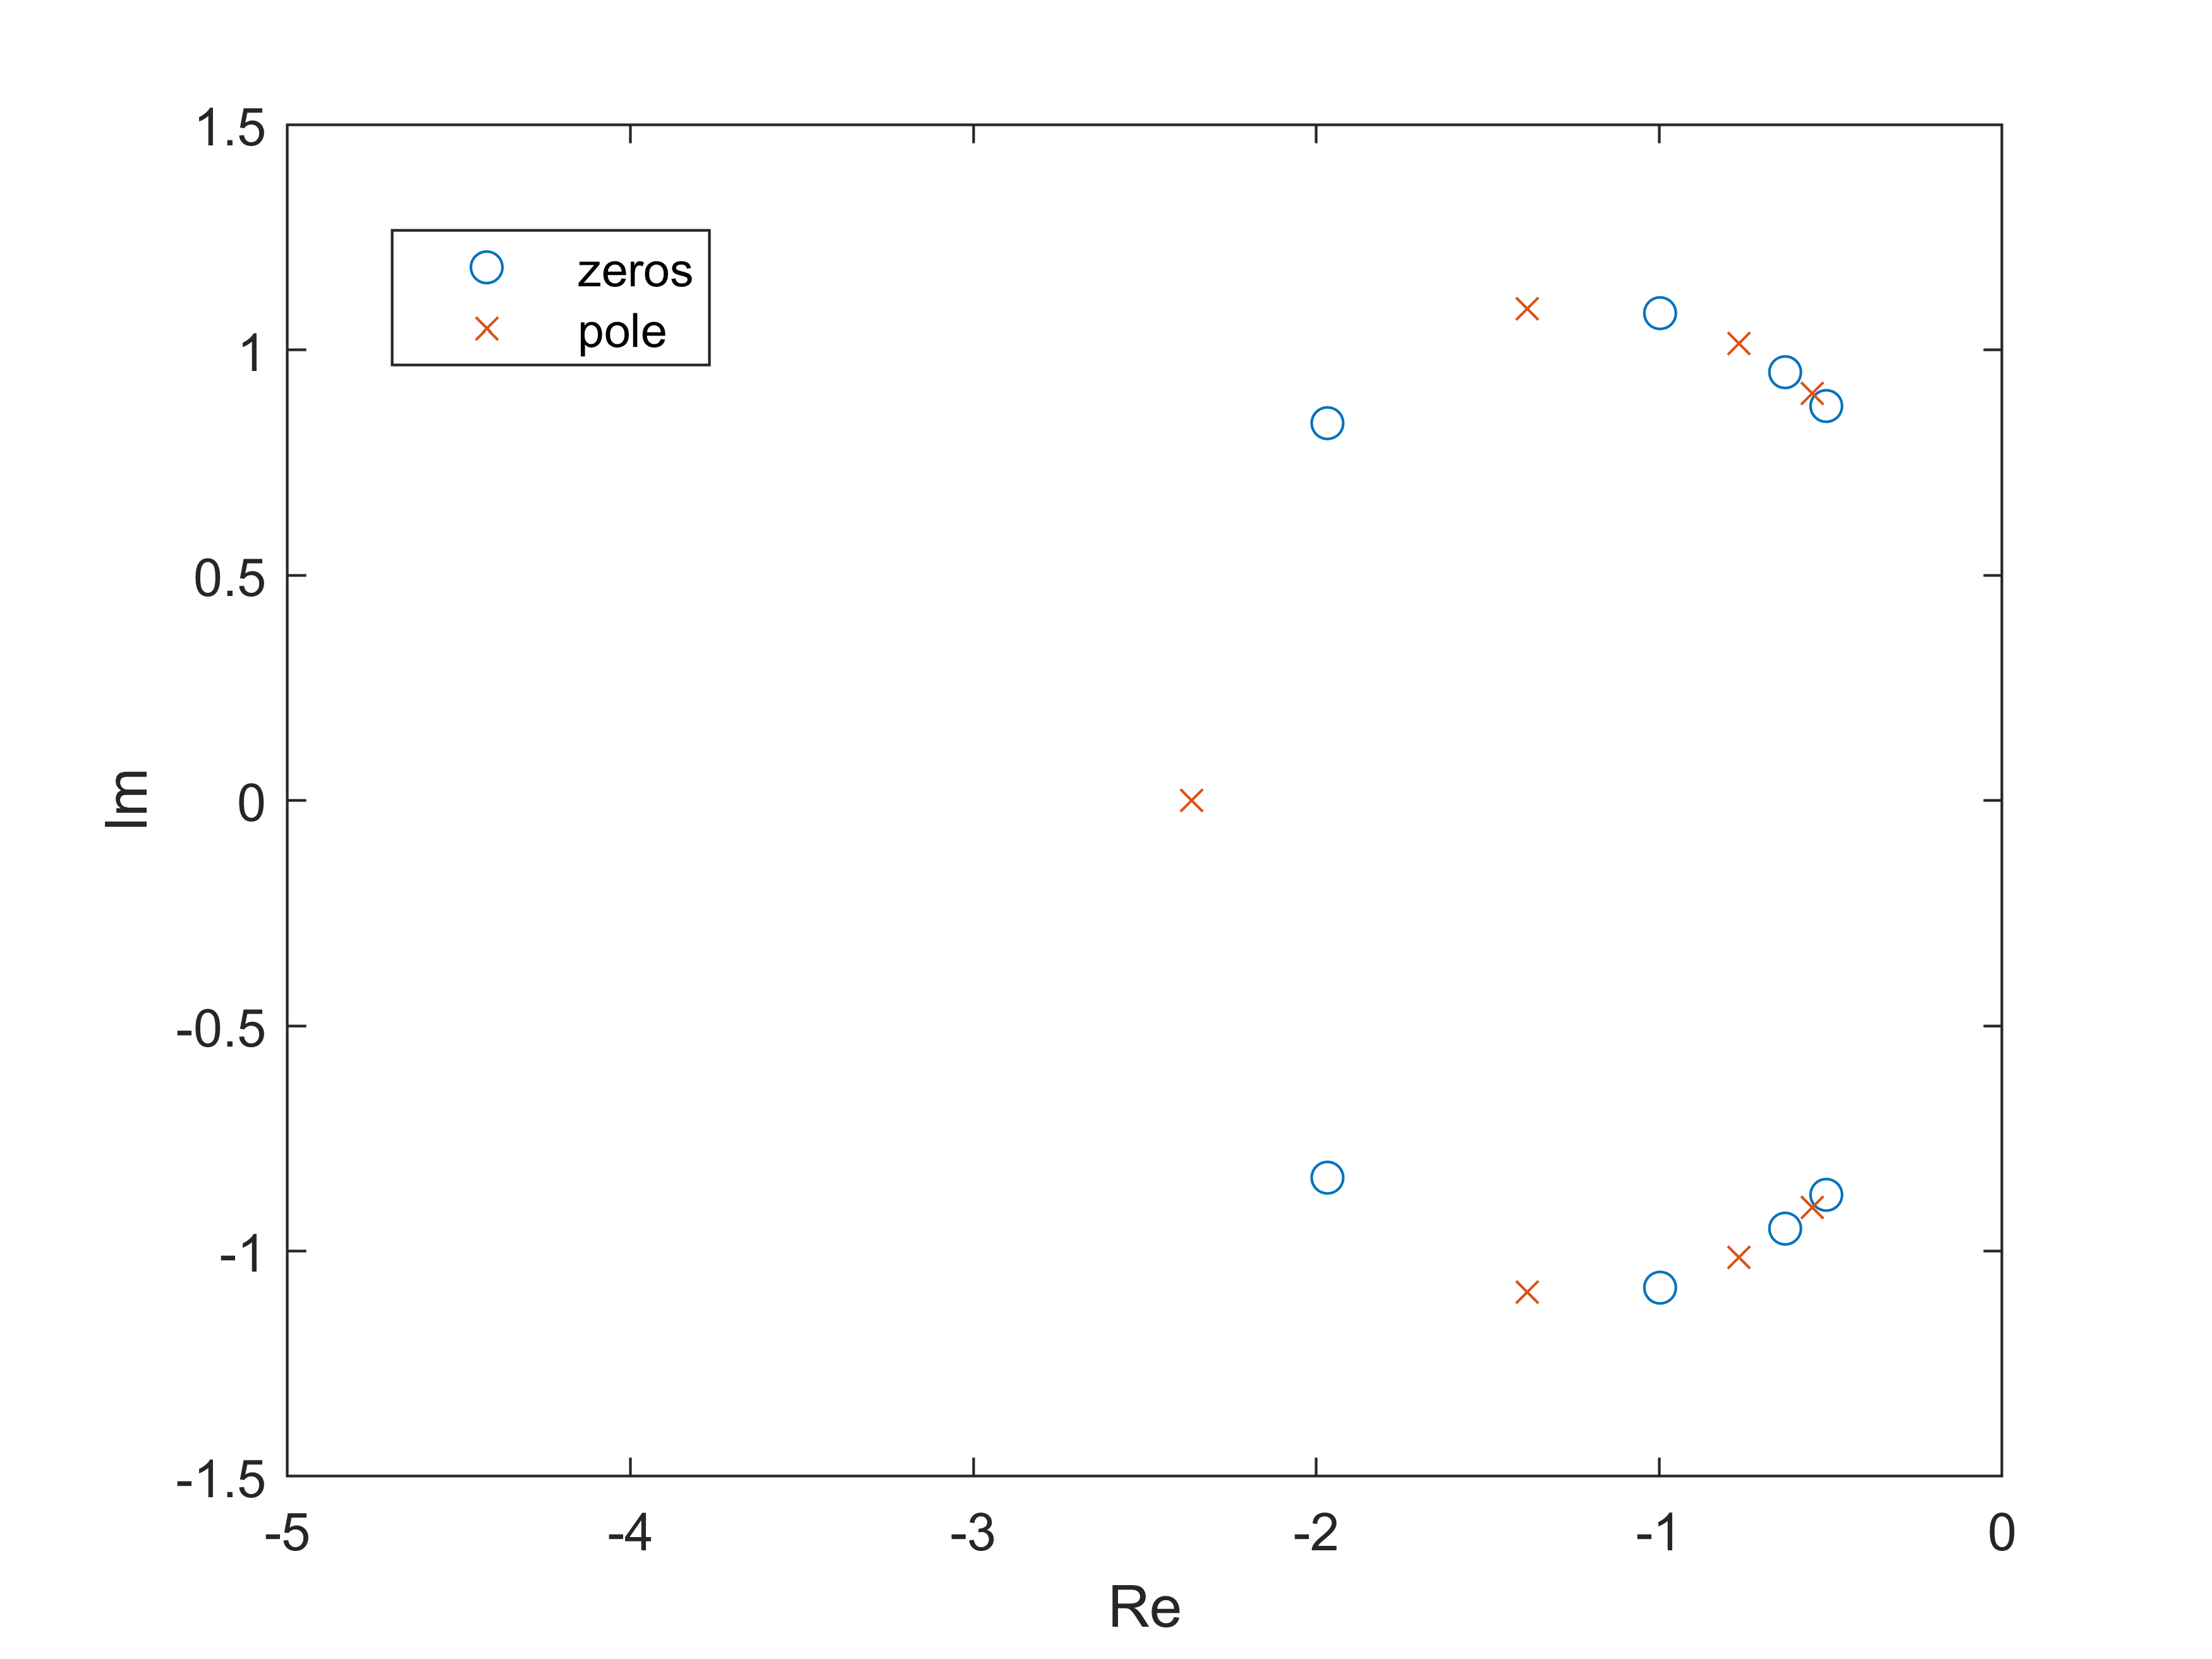
\includegraphics[width=\textwidth]{Files/q5,f6,8_ring.png}
    \caption{Pole-Zero plot of $R_{8,8}(f_6)$ near origin}
        \end{minipage}
\end{figure}
\noindent When $L$ is odd, there is a pole on the positive real axis with large $|z|$, and when $L$ increases by $1$, this pole will move to the negative real axis and $|z|$ is roughly tripled. There is also an alternating pole and zero on the negative real axis close to the origin which moves closer to the origin every time $L$ goes up by $1$. When $L$ is odd, it's a zero; and when $L$ is even, it's a pole.\\
We shall call this point $p$. There is a symmetry of zeros/poles over the real axis which are distributed in a ring liked shape, as shown in figure 24 and 26. And when $p$ is a pole, the nearest pair of points are zeroes; and when $p$ is a zero, the nearest pair of points are poles.\\\\
\noindent For \textbf{$f_1=(1+z)^{(1/2)}$}, we know that it has a branch point on $z=(-1,0)$ and a branch cut from $(-1,0)$ to $(-\infty,0)$ (the negative real axis). We note that all of its poles and zeros lie on the branch cut, with a high density of points near $(-1,0)$ and an increasing range in $|z|$. Hence, the positions of poles and zeros correspond to the branch cut and branch point of $f_1$. We can see this graphically on figure 13 and 14.\\\\
\noindent For \textbf{$f_3=(1+z)^{(-1/2)}$}, there is again a branch point at $z=(-1,0)$ and a branch cut from $(-1,0)$ to $(-\infty,0)$. Hence, the positions of poles and zeros correspond to the branch cut and branch point of $f_3$, just as in the case of $f_1$. We can see this graphically on figure 15 and 16.\\\\
\noindent For \textbf{$f_4=e^z$}, we know that $e^z$ and $e^{-z}$ are both entire functions, therefore they have no poles. And since they are reciprocal to each other, $e^z$ has no zeros either. And since it's entire, it contains no branch points or branch cuts. So the zeros and poles of $R_{L,L}(f_4)$ do \underline{not} correspond to any poles, zeros, branch points or branch cuts of $f_4$.\\\\
\noindent For \textbf{$f_5=e^z/(1+z)$}, there is a pole at $z=(-1,0)$, no zeros, branch cuts or branch points. There is also a pole in $R_{L,L}(f_5)$ at $z=(-1,0)$, so this pole in $R_{L,L}$ correspond to the pole in $f_5$. However, the other poles and zeros do not correspond to any poles, zeros, branch points or branch cuts of $f_4$. We can see this graphical on figure 19,20,21,22.\\\\
\noindent For \textbf{$f_6=(1+z+z^2)^{(1/2)}$}, we note that $f_6$ can be written as $((z-(-1/2-\sqrt{3}i/2))(z-(1/2+\sqrt{3}i/2)))^{\frac{1}{2}}$, hence it has two branch points at $(-1/2,\pm\sqrt{3}/2)$ and it has a branch cut between these two branch points. In the meanwhile if we make the change of variable $x=\frac{1}{z}$, we see that it also has a branch point at $\infty$. So the pole that's moving towards $\infty$ as $L$ increases corresponds to the branch point at infinity. And we can show the ring-shaped curve of points correspond to the two branch points and the branch cut between them by plotting the branch cut over figure 26.\\\\

\newpage
\noindent Therefore, almost all of the poles and zeros in $R_{L,L}(f_4)$ and $R_{L,L}(f_5)$ are 'anomalous' points, except $(-1,0)$ for $f_5$. For $f_1$ and $f_3$, if we increase $L$ to be large enough, then such points start to appear, e.g. when $L=20$,
\begin{figure}[H]
\centering
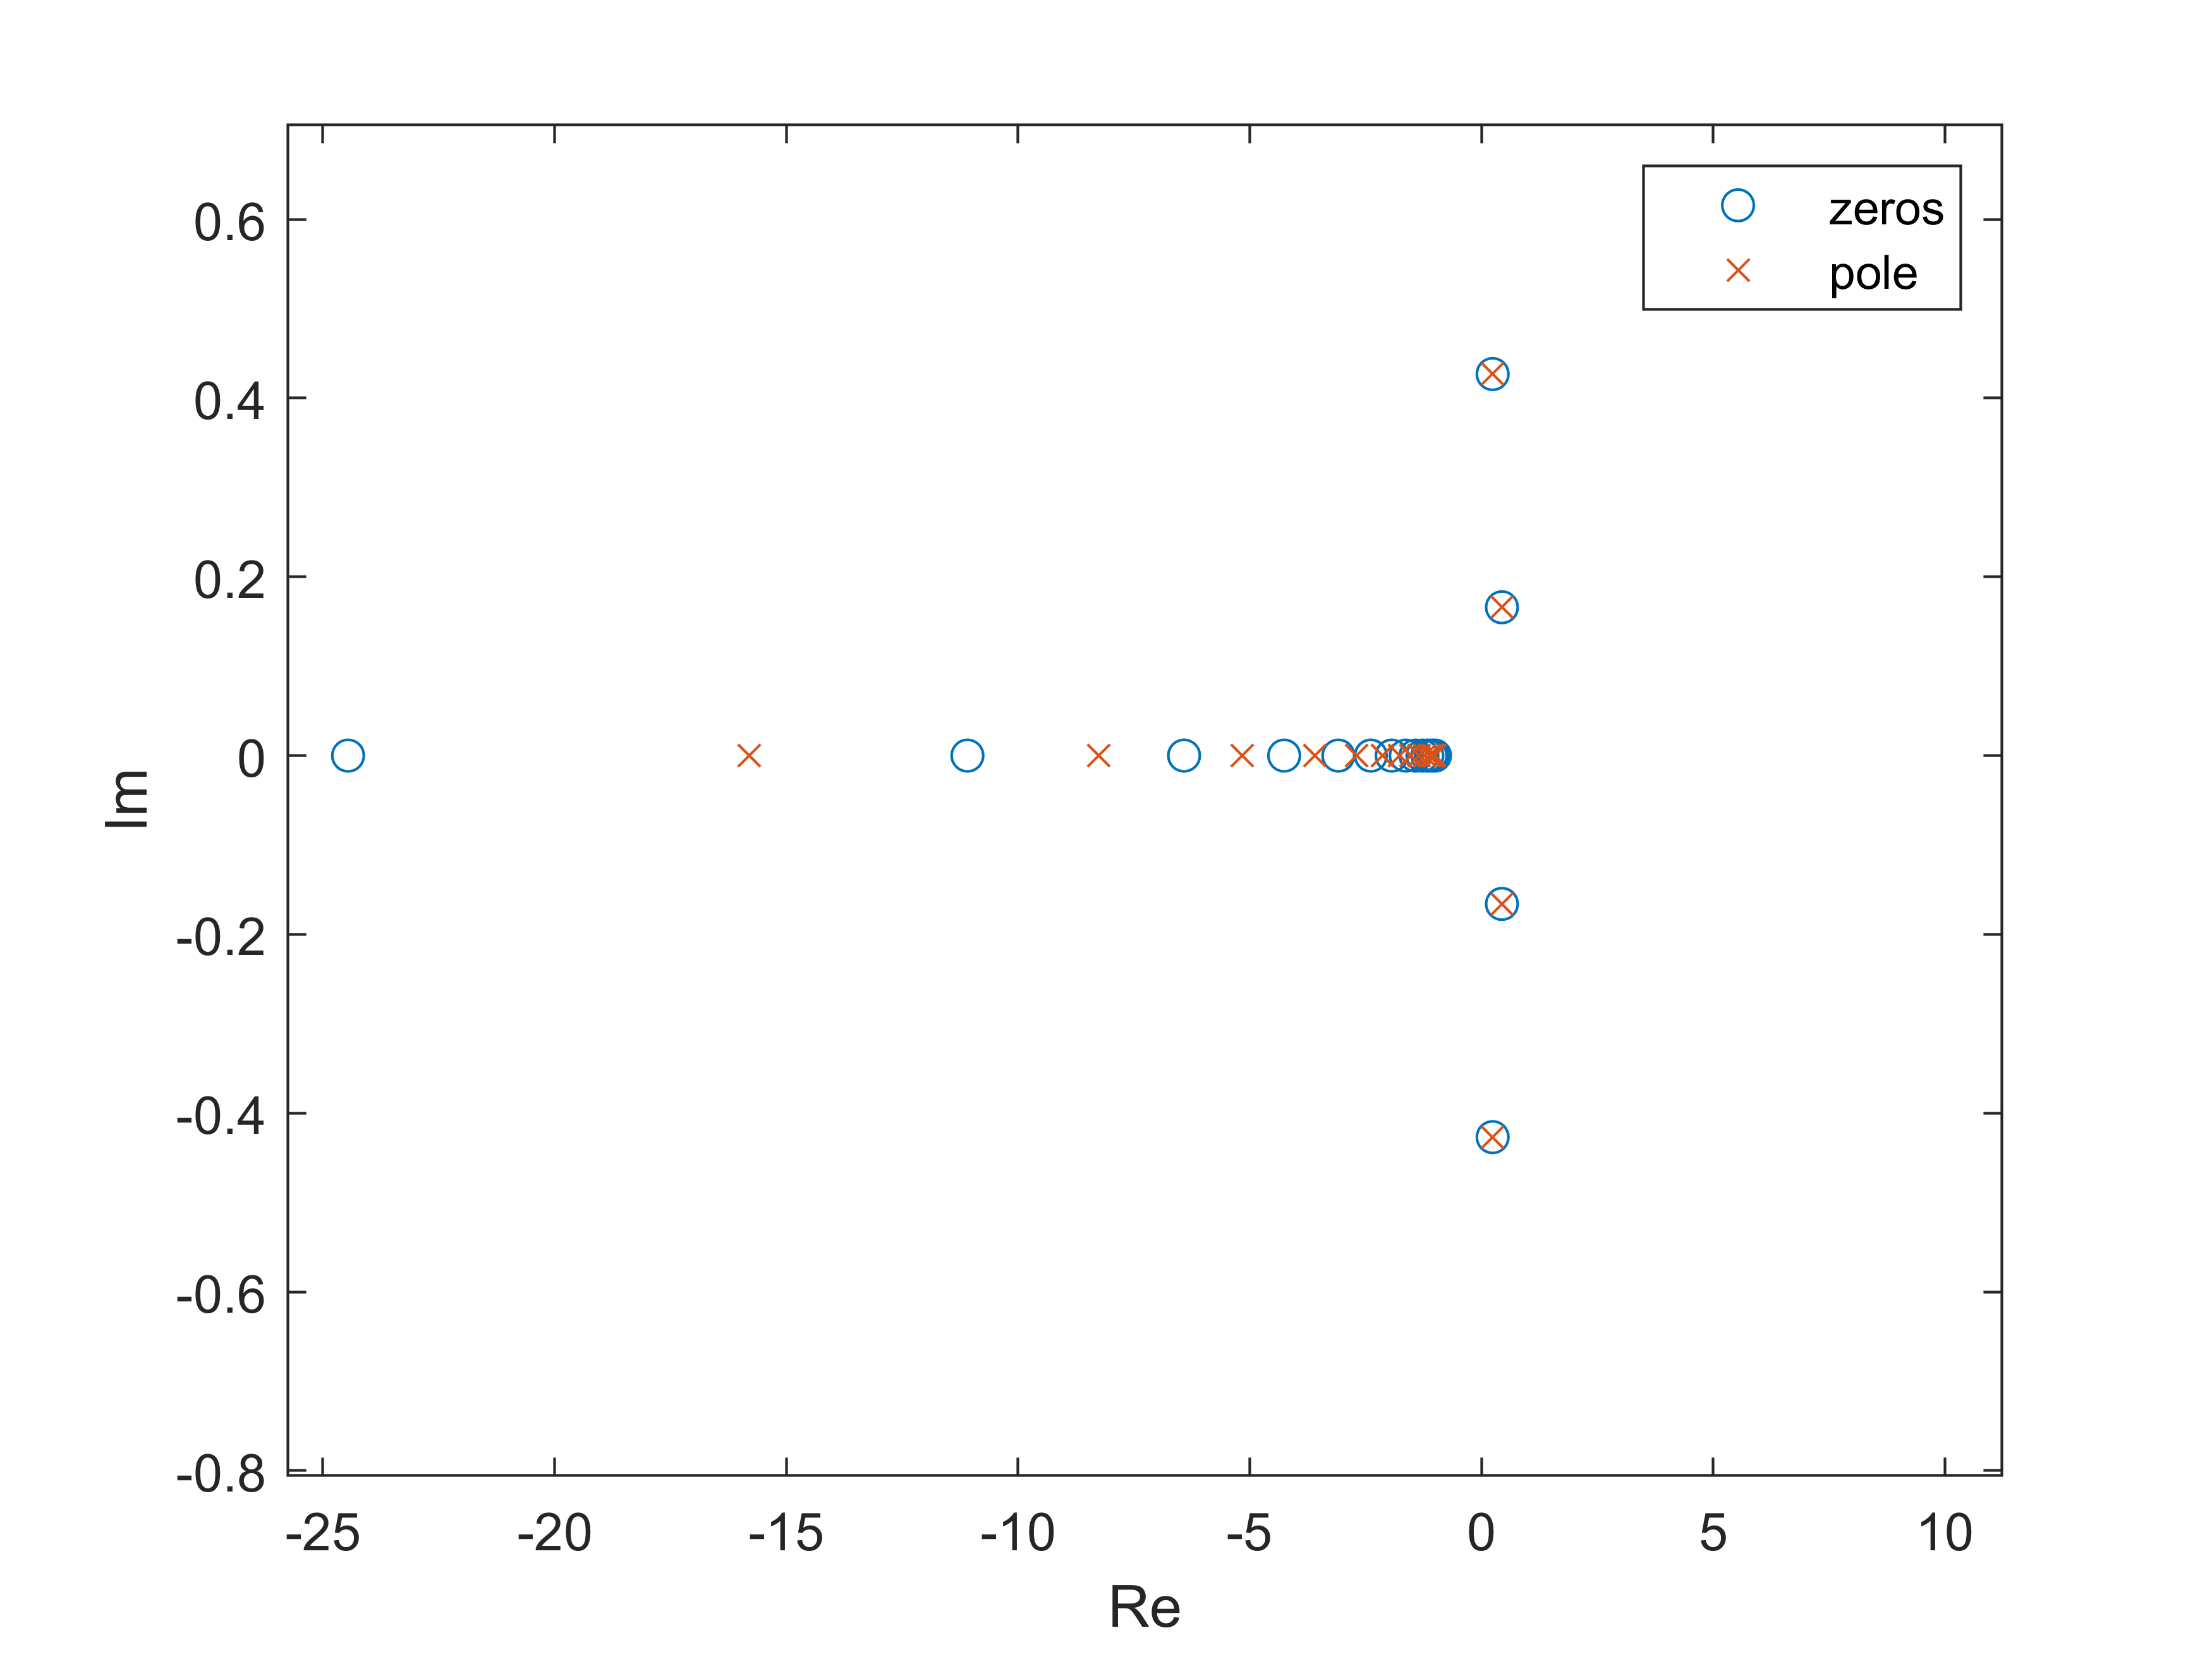
\includegraphics[width=0.5\textwidth]{Files/q5,f1,20.png}
\caption{Pole-Zero plot of $R_{20,20}(f_1)$}
\end{figure}
\noindent We can see four such points not corresponding to the branch cut, lying on the imaginary axis.\\
What we do notice however, is such 'anomolous' zeros and poles for $f_1$ and $f_3$ overlap each other, which means that they are not actual poles and zeros of $R_{L,L}(f_1)$, since the factors would cancel when we divide the numerator polynomial by the denominator polynomial.\\



\newpage
\section*{Files}
\subsection*{i) Table of pade approximants errors using numeric calculation}
    \begin{tabular}{c|c|c}
    $L$ & $R_{L,L}(1)$ & e=$|\sqrt{2}-R_{L,L}(1)|$\\
    \hline
     1    & 1.400000000000000    &  1.421356237309523e-02\\
     2    & 1.413793103448276    & 4.204589248193447e-04\\
     3    & 1.414201183431953    & 1.237894114258786e-05\\
     4    & 1.414213197969543    & 3.644035520000699e-07\\
     5    & 1.414213551646055    & 1.072704058913132e-08\\
     6    & 1.414213562057320    & 3.157747396898003e-10\\
     7    & 1.414213562363799    & 9.295675340581511e-12\\
     8    & 1.414213562372821    & 2.737809978725636e-13\\
     9    & 1.414213562373087    & 7.993605777301127e-15\\
     10   & 1.414213562373095    & 2.220446049250313e-16\\
     11   & 1.414213562373095    &                     0\\
     12   & 1.414213562373095    & 2.220446049250313e-16
    \end{tabular}
\subsection*{ii) Table of pade approximants errors using symbolic calculation}
    \begin{tabular}{c|c|c}
    $L$ & $R_{L,L}(1)$ & e=$|\sqrt{2}-R_{L,L}(1)|$\\
    \hline
    1  &   1.400000000000000    & 1.421356237309523e-02\\
     2  &   1.413793103448276 &    4.204589248193447e-04\\
     3  &   1.414201183431953 &    1.237894114258786e-05\\
     4  &   1.414213197969543 &    3.644035520000699e-07\\
     5  &   1.414213551646055 &    1.072704036708672e-08\\
     6  &   1.414213562057320 &    3.157747396898003e-10\\
     7  &   1.414213562363799 &    9.295675340581511e-12\\
     8  &   1.414213562372821 &    2.737809978725636e-13\\
     9  &   1.414213562373087 &    8.215650382226158e-15\\
     10  &   1.414213562373095 &    4.440892098500626e-16\\
     11  &   1.414213562373095 &                        0\\
     12  &   1.414213562373095 &                        0\\
     13  &   1.414213562373095 &                        0\\
     14  &   1.414213562373095 &                        0\\
     15  &   1.414213562373095 &                        0\\
     16  &   1.414213562373095 &                        0\\
     17  &   1.414213562373095 &                        0\\
     18  &   1.414213562373095 &    4.440892098500626e-16\\
     19  &   1.414213562373095 &    2.220446049250313e-16\\
     20  &   1.414213562373095 &    2.220446049250313e-16
    \end{tabular}


\newpage
\section*{Programs}
\subsection*{i) CoefSolver.m}
\lstdefinestyle{myCustomMatlabStyle}{
  language=Matlab,
  stepnumber=1,
  numbersep=10pt,
  tabsize=4,
  showspaces=false,
  showstringspaces=false
}
\lstset{basicstyle=\footnotesize,style=myCustomMatlabStyle}
\begin{lstlisting}
function [R] = CoefSolver(f,x0,L,M,y)
% parameters:
% R is the pade approximant at y
% f is the orginal equation
% x0 is where the taylor expansion is based around
% L is the max order term of the numerator
% M is the max order term of the denominator
% y is the value we want to evaluate the approximant at
syms x
% compute the L+M+1 term of the taylor series
fexp = taylor(f,x,x0,'Order', L+M+1);
% extract the coefficients
c = sym2poly(fexp);
% reverse the order, now it's ascending
c = c(L+M+1:-1:1);
% symbolic calculation to avoid numerical error
c = sym(c);
% A is the matrix of simultaneous equation in c
A = zeros(M);
% B is vector of (-c_L+1,...,-C_L+M) 
B = [-c(L+2:L+M+1)]';    
% c(L+2)=c_(L+1) and c(L+M+1)=c_(L+M)
% since indexing start from 1 and c(1)=c_0

for r = L+1:L+M
    upper_limit = min(r,M);
    % update the matrix with coef c_(r-k)
    % if index larger than min(r,M), then A(index)=0
    for k = 1 : upper_limit
        A(r-L,k) = c(r-k+1);
    end
end
% symbolic calculation to avoid numerical error
A = sym(A);
% q is the coefficients of the denominator start from q1
% q is the solution to Ax=B, row vector
q = mldivide(A,B)';

% p is the coefficients of the numerator start from p0
% now we find the coefficients p
p = zeros(1,L+1);
p(1) = c(1);
% equation 5
for k = 1:L
    upper_limit = min(k,M);
    % temporary result of sum of q_s*c_(k-s)
    temp = 0;
    for s = 1 : upper_limit
        temp = temp + q(s)*c(k-s+1);
    end
    p(k+1) = c(k+1)+ temp;
end

% reverese order to descending powers
p = p(L+1:-1:1);
q = q(M:-1:1);
% set the q_0 to be zero for easier conversion to polynomials
q(M+1) = 1;
q = double(q);
% evaluate R at point y
R = polyval(p,y)/polyval(q,y);


\end{lstlisting}
\subsection*{ii) RootFinder.m}
\lstdefinestyle{myCustomMatlabStyle}{
  language=Matlab,
  stepnumber=1,
  numbersep=10pt,
  tabsize=4,
  showspaces=false,
  showstringspaces=false
}
\lstset{basicstyle=\footnotesize,style=myCustomMatlabStyle}
\begin{lstlisting}
function [r] = RootFinder(f)
% f is the coefficients of the polynomial we want to solve
% f should be in descending order
% r is the complex roots of the polynomial

r = roots(f);

\end{lstlisting}
\subsection*{iii) q1.m}
\lstdefinestyle{myCustomMatlabStyle}{
  language=Matlab,
  stepnumber=1,
  numbersep=10pt,
  tabsize=4,
  showspaces=false,
  showstringspaces=false
}
\lstset{basicstyle=\footnotesize,style=myCustomMatlabStyle}
\begin{lstlisting}
format long
range_N = [10:10:150]';     % the range of N we wish to test with
NumTestN = numel(range_N);
partial_sum = zeros(NumTestN,1);   % to store the results for partial sums
errors = zeros(NumTestN,1);        % to store the results for error term
for i = 1:numel(range_N)
    N = range_N(i);     % N is the number of terms we wish to add
    c = zeros(N,1);   % c stores the value of c_k for k=1,...N
    c(1) = 1/2;  % value of c_1
    for k = 2:N
        % temp is (2k-3)*(2k-1)*...*3*1
        temp = 1;
        for j = 1:2:(2*k-3)
            temp = temp*j;
        end
        % calculate c_k
        c(k) = ((-1)^(k-1))*temp/...
            (factorial(k)*2^(k));
    end
    temp_sum = 1+sum(c);     % need to add c_0 to the partial sum  
    % compare values between sqrt(2) and the partial sum
    temp_error = abs(sqrt(2)-temp_sum);  
    partial_sum(i) = temp_sum;
    errors(i) = temp_error;
end
disp([range_N,partial_sum,errors])


\end{lstlisting}
\subsection*{iv) q2.m}
\lstdefinestyle{myCustomMatlabStyle}{
  language=Matlab,
  stepnumber=1,
  numbersep=10pt,
  tabsize=4,
  showspaces=false,
  showstringspaces=false
}
\lstset{basicstyle=\footnotesize,style=myCustomMatlabStyle}
\begin{lstlisting}
format long e
syms x
range_L = 1:20;  % max order of numerator
f = @(x) (1+x)^(1/2);   % equation of f_1(x)
% R stores the pade approximations at different values of L
R = zeros(numel(range_L),1);
for i = 1:numel(range_L)
    L = range_L(i);
    R(i) = CoefSolver(f,0,L,L,1);       % find the approximation at x=1
end
disp([range_L',R,abs(sqrt(2)-R)])
% plot log-log of L against error
plot(log(range_L), log(abs(sqrt(2)-R)))
xlabel('log(L)')
ylabel('log(error)')
% plot log(error) against L
figure()
plot(range_L, log(abs(sqrt(2)-R)))
xlabel('L')
ylabel('log(error)')


\end{lstlisting}
\subsection*{v) q3\textunderscore power\textunderscore series.m}
\lstdefinestyle{myCustomMatlabStyle}{
  language=Matlab,
  stepnumber=1,
  numbersep=10pt,
  tabsize=4,
  showspaces=false,
  showstringspaces=false
}
\lstset{basicstyle=\footnotesize,style=myCustomMatlabStyle}
\begin{lstlisting}
% power series estimate for f_1(x), expansion about x=0
range_N = [0,1];      % range of N we want to test
% plot against x from 1 to 100 with increment of 0.1
x = linspace(1,100,10000); 
for i = 1:numel(range_N)
    result = zeros(numel(x),1);
    N = range_N(i);     % N is the number of terms we wish to add
    c = zeros(N,1);   % c stores the value of c_k for k=1,...N
    c(1) = 1/2;  % value of c_1
    for k = 2:N
        % temp is (2k-3)*(2k-1)*...*3*1
        temp = 1;
        for j = 1:2:(2*k-3)
            temp = temp*j;
        end
        % calculate c_k
        c(k) = ((-1)^(k-1))*temp/...
            (factorial(k)*2^(k));
    end
    % reverse the order of c_k to descending
    c = c(N:-1:1);
    % c_0 = 1
    c(N+1) = 1;
    % evaluate the power series at points of x
    for l = 1:numel(x)
        result(l) = polyval(c,x(l));
    end
    plot(x,result,'DisplayName', sprintf('N=%g',N))
    hold on
end
% compare with f_1(x)
plot(x,(1+x).^(1/2),'DisplayName','f(x)')
legend()

\end{lstlisting}
\subsection*{vi) CoefPade.m}
\lstdefinestyle{myCustomMatlabStyle}{
  language=Matlab,
  stepnumber=1,
  numbersep=10pt,
  tabsize=4,
  showspaces=false,
  showstringspaces=false
}
\lstset{basicstyle=\footnotesize,style=myCustomMatlabStyle}
\begin{lstlisting}
function [p,q] = CoefPade(f,x0,L,M)
% parameters:
% p is the coefficient of the numerator
% q is the coefficient of the denominator
% f is the orginal equation
% x0 is where the taylor expansion is based around
% L is the max order term of the numerator
% M is the max order term of the denominator
syms x
% compute the L+M+1 term of the taylor series
fexp = taylor(f,x,x0,'Order', L+M+1);
% extract the coefficients
c = sym2poly(fexp);
% reverse the order, now it's ascending
c = c(L+M+1:-1:1);
% symbolic calculation to avoid numerical error
c = sym(c);
% A is the matrix of simultaneous equation in c
A = zeros(M);
% B is vector of (-c_L+1,...,-C_L+M) 
B = [-c(L+2:L+M+1)]';    
% c(L+2)=c_(L+1) and c(L+M+1)=c_(L+M)
% since indexing start from 1 and c(1)=c_0

for r = L+1:L+M
    upper_limit = min(r,M);
    % update the matrix with coef c_(r-k)
    % if index larger than min(r,M), then A(index)=0
    for k = 1 : upper_limit
        A(r-L,k) = c(r-k+1);
    end
end
% symbolic calculation to avoid numerical error
A = sym(A);
% q is the coefficients of the denominator start from q1
% q is the solution to Ax=B, row vector
q = mldivide(A,B)';

% p is the coefficients of the numerator start from p0
% now we find the coefficients p
p = zeros(1,L+1);
p(1) = c(1);
% equation 5
for k = 1:L
    upper_limit = min(k,M);
    % temporary result of sum of q_s*c_(k-s)
    temp = 0;
    for s = 1 : upper_limit
        temp = temp + q(s)*c(k-s+1);
    end
    p(k+1) = c(k+1)+ temp;
end

% reverese order to descending powers
p = p(L+1:-1:1);
q = q(M:-1:1);
% set the q_0 to be 1 for easier conversion to polynomials
q(M+1) = 1;
q = double(q);

\end{lstlisting}
\subsection*{vii) q3\textunderscore pade.m}
\lstdefinestyle{myCustomMatlabStyle}{
  language=Matlab,
  stepnumber=1,
  numbersep=10pt,
  tabsize=4,
  showspaces=false,
  showstringspaces=false
}
\lstset{basicstyle=\footnotesize,style=myCustomMatlabStyle}
\begin{lstlisting}
format long e
syms x
range_L = [1,5,10];  % max order of numerator
f = @(x) (1+x)^(1/2);   % equation of f_1(x)
x = linspace(1,100,10000);
for i = 1:numel(range_L)
    L = range_L(i);
    % R stores the pade approximations at different x
    R = zeros(numel(x),1);
    % cache the coefficients
    [p,q] = CoefPade(f,0,L,L);
    for j = 1: numel(x)
        R(j) = polyval(p,x(j))/polyval(q,x(j));   % find the approximation at x(j)
    end
    plot(x,R,'DisplayName',sprintf('L=%g',L))
    hold on
end
plot(x,(1+x).^(1/2),'DisplayName', 'f(x)')
legend()

\end{lstlisting}
\newpage
\subsection*{viii) q3\textunderscore pade \textunderscore points.m}
\lstdefinestyle{myCustomMatlabStyle}{
  language=Matlab,
  stepnumber=1,
  numbersep=10pt,
  tabsize=4,
  showspaces=false,
  showstringspaces=false
}
\lstset{basicstyle=\footnotesize,style=myCustomMatlabStyle}
\begin{lstlisting}
format long e
syms x
range_L = [1:20];  % max order of numerator
f = @(x) (1+x)^(1/2);   % equation of f_1(x)
x = [10,100];
for j = 1:numel(x)
        % R stores the pade approximations at different L
        R = zeros(numel(range_L),1);
        error = zeros(numel(range_L),1);
    for i = 1:numel(range_L)
        L = range_L(i);
        % calculating R,error at diferent levels of L
        R(i) = CoefSolver(f,0,L,L,x(j));
        error(i) = abs(R(i)-(1+x(j))^(1/2));
    end
        % plotting the error at x(j) against range of L
        plot(range_L,error,'DisplayName',sprintf('x=%g',x(j)))
        legend()
        figure()
end

\end{lstlisting}
\subsection*{ix) q4\textunderscore pade.m}
\lstdefinestyle{myCustomMatlabStyle}{
  language=Matlab,
  stepnumber=1,
  numbersep=10pt,
  tabsize=4,
  showspaces=false,
  showstringspaces=false
}
\lstset{basicstyle=\footnotesize,style=myCustomMatlabStyle}
\begin{lstlisting}
format long e
x = linspace(0,20,200);
range_L = [3,7,11];  % order of L we wish to plot at
for l = 1:numel(range_L)
    L = range_L(l);
    c = zeros(1,2*L+1);     % stores from c_0 to c_L+M+1
    R = zeros(numel(x),1);
    % find the coefficients directly
    for i = 1:2*L+1
        c(i)= ((-1)^(i-1))*factorial(i-1);
    end
    for j = 1:numel(x)
        R(j) = CoefSolverPS(c,L,L,x(j));    % find pade estimation at x(j)
    end
    plot(x,R,'DisplayName',sprintf('L=%g',L))
    hold on
end
% the numerical integration result from project sheet
x_num = [0.1,0.2,0.3,0.4,0.5,0.6,0.7,0.8,0.9,1,2,3,4,5,6,7,8,9,10,11,12,13,14,15,16,17,18,19,20];
y_num = [0.91563334, 0.85211088, 0.80118628, 0.75881459, 0.72265723, 0.69122594, 0.66351027...
    0.63879110, 0.61653779, 0.59634736, 0.46145532, 0.38560201, 0.33522136, 0.29866975,...
    0.27063301, 0.24828135, 0.22994778, 0.21457710, 0.20146425, 0.19011779,0.18018332,...
    0.17139800, 0.16356229, 0.15652164, 0.15015426, 0.14436271, 0.13906806, 0.13420555, 0.12972152];
plot(x_num,y_num,'DisplayName', 'f2(x)')
legend()

\end{lstlisting}
\newpage
\subsection*{x) CoefSolverPS.m}
\lstdefinestyle{myCustomMatlabStyle}{
  language=Matlab,
  stepnumber=1,
  numbersep=10pt,
  tabsize=4,
  showspaces=false,
  showstringspaces=false
}
\lstset{basicstyle=\footnotesize,style=myCustomMatlabStyle}
\begin{lstlisting}
function [R] = CoefSolverPS(c,L,M,y)
% parameters:
% R is the pade approximant at y
% c is the power series truncated to L+M+1 terms
% L is the max order term of the numerator
% M is the max order term of the denominator
% y is the value we want to evaluate the approximant at
% symbolic calculation to avoid numerical error
c = sym(c);
% A is the matrix of simultaneous equation in c
A = zeros(M);
% B is vector of (-c_L+1,...,-C_L+M) 
B = [-c(L+2:L+M+1)]';    
% c(L+2)=c_(L+1) and c(L+M+1)=c_(L+M)
% since indexing start from 1 and c(1)=c_0

for r = L+1:L+M
    upper_limit = min(r,M);
    % update the matrix with coef c_(r-k)
    % if index larger than min(r,M), then A(index)=0
    for k = 1 : upper_limit
        A(r-L,k) = c(r-k+1);
    end
end
% symbolic calculation to avoid numerical error
A = sym(A);
% q is the coefficients of the denominator start from q1
% q is the solution to Ax=B, row vector
q = mldivide(A,B)';

% p is the coefficients of the numerator start from p0
% now we find the coefficients p
p = zeros(1,L+1);
p(1) = c(1);
% equation 5
for k = 1:L
    upper_limit = min(k,M);
    % temporary result of sum of q_s*c_(k-s)
    temp = 0;
    for s = 1 : upper_limit
        temp = temp + q(s)*c(k-s+1);
    end
    p(k+1) = c(k+1)+ temp;
end

% reverese order to descending powers
p = p(L+1:-1:1);
q = q(M:-1:1);
% set the q_0 to be 1 for easier conversion to polynomials
q(M+1) = 1;
q = double(q);
% evaluate R at point y
R = polyval(p,y)/polyval(q,y);

\end{lstlisting}
\newpage
\subsection*{xi) q4\textunderscore power\textunderscore series.m}
\lstdefinestyle{myCustomMatlabStyle}{
  language=Matlab,
  stepnumber=1,
  numbersep=10pt,
  tabsize=4,
  showspaces=false,
  showstringspaces=false
}
\lstset{basicstyle=\footnotesize,style=myCustomMatlabStyle}
\begin{lstlisting}
% truncation power
range_N = [4,7];      % range of N we want to test
% plot against x from 0 to 20 with increment of 0.1
x = linspace(0,1,50); 
for i = 1:numel(range_N)
    result = zeros(numel(x),1);
    N = range_N(i);     % N is the number of terms we wish to add
    c = zeros(N,1);   % c stores the value of c_k for k=1,...N
    % find the coefficients directly
    for j = 1:N
        c(j)= ((-1)^(j))*factorial(j);
    end
    % reverse the order of c_k to descending
    c = c(N:-1:1);
    % c_0 = 1
    c(N+1) = 1;
    % evaluate the power series at points of x
    for l = 1:numel(x)
        result(l) = polyval(c,x(l));
    end
    plot(x,result,'DisplayName', sprintf('N=%g',N))
    hold on
end
% compare with f_1(x)
x_num = [0.1,0.2,0.3,0.4,0.5,0.6,0.7,0.8,0.9,1];
y_num = [0.91563334, 0.85211088, 0.80118628, 0.75881459, 0.72265723, 0.69122594, 0.66351027...
    0.63879110, 0.61653779, 0.59634736];
plot(x_num,y_num,'DisplayName', 'f2(x)')
legend()
ylim([0,1])

\end{lstlisting}
\subsection*{xii) q5.m}
\lstdefinestyle{myCustomMatlabStyle}{
  language=Matlab,
  stepnumber=1,
  numbersep=10pt,
  tabsize=4,
  showspaces=false,
  showstringspaces=false
}
\lstset{basicstyle=\footnotesize,style=myCustomMatlabStyle}
\begin{lstlisting}
format long
syms x
f = @(x) (1+x+x^2)^(1/2);   % fill in equation of f_i(x), i=1,3,4,5,6
range_L = [7,8];      % range of L we want to look at
for i = 1:numel(range_L)    
    L = range_L(i);
    [p,q] = CoefPade(f,0,L,L); % coefficients of numerator and denominator
    zeros = complex(RootFinder(p));  % zeros are roots of the numerator poly
    poles = complex(RootFinder(q));  % poles are roots of the denominator poly
    figure()
    plot(zeros,'o','DisplayName','zeros')
    hold on
    plot(poles,'x','DisplayName','pole')
    legend()
end

\end{lstlisting}

\end{document}
